% Options for packages loaded elsewhere
% Options for packages loaded elsewhere
\PassOptionsToPackage{unicode}{hyperref}
\PassOptionsToPackage{hyphens}{url}
\PassOptionsToPackage{dvipsnames,svgnames,x11names}{xcolor}
%
\documentclass[
  letterpaper,
  DIV=11,
  numbers=noendperiod]{scrreprt}
\usepackage{xcolor}
\usepackage{amsmath,amssymb}
\setcounter{secnumdepth}{5}
\usepackage{iftex}
\ifPDFTeX
  \usepackage[T1]{fontenc}
  \usepackage[utf8]{inputenc}
  \usepackage{textcomp} % provide euro and other symbols
\else % if luatex or xetex
  \usepackage{unicode-math} % this also loads fontspec
  \defaultfontfeatures{Scale=MatchLowercase}
  \defaultfontfeatures[\rmfamily]{Ligatures=TeX,Scale=1}
\fi
\usepackage{lmodern}
\ifPDFTeX\else
  % xetex/luatex font selection
\fi
% Use upquote if available, for straight quotes in verbatim environments
\IfFileExists{upquote.sty}{\usepackage{upquote}}{}
\IfFileExists{microtype.sty}{% use microtype if available
  \usepackage[]{microtype}
  \UseMicrotypeSet[protrusion]{basicmath} % disable protrusion for tt fonts
}{}
\makeatletter
\@ifundefined{KOMAClassName}{% if non-KOMA class
  \IfFileExists{parskip.sty}{%
    \usepackage{parskip}
  }{% else
    \setlength{\parindent}{0pt}
    \setlength{\parskip}{6pt plus 2pt minus 1pt}}
}{% if KOMA class
  \KOMAoptions{parskip=half}}
\makeatother
% Make \paragraph and \subparagraph free-standing
\makeatletter
\ifx\paragraph\undefined\else
  \let\oldparagraph\paragraph
  \renewcommand{\paragraph}{
    \@ifstar
      \xxxParagraphStar
      \xxxParagraphNoStar
  }
  \newcommand{\xxxParagraphStar}[1]{\oldparagraph*{#1}\mbox{}}
  \newcommand{\xxxParagraphNoStar}[1]{\oldparagraph{#1}\mbox{}}
\fi
\ifx\subparagraph\undefined\else
  \let\oldsubparagraph\subparagraph
  \renewcommand{\subparagraph}{
    \@ifstar
      \xxxSubParagraphStar
      \xxxSubParagraphNoStar
  }
  \newcommand{\xxxSubParagraphStar}[1]{\oldsubparagraph*{#1}\mbox{}}
  \newcommand{\xxxSubParagraphNoStar}[1]{\oldsubparagraph{#1}\mbox{}}
\fi
\makeatother

\usepackage{color}
\usepackage{fancyvrb}
\newcommand{\VerbBar}{|}
\newcommand{\VERB}{\Verb[commandchars=\\\{\}]}
\DefineVerbatimEnvironment{Highlighting}{Verbatim}{commandchars=\\\{\}}
% Add ',fontsize=\small' for more characters per line
\usepackage{framed}
\definecolor{shadecolor}{RGB}{241,243,245}
\newenvironment{Shaded}{\begin{snugshade}}{\end{snugshade}}
\newcommand{\AlertTok}[1]{\textcolor[rgb]{0.68,0.00,0.00}{#1}}
\newcommand{\AnnotationTok}[1]{\textcolor[rgb]{0.37,0.37,0.37}{#1}}
\newcommand{\AttributeTok}[1]{\textcolor[rgb]{0.40,0.45,0.13}{#1}}
\newcommand{\BaseNTok}[1]{\textcolor[rgb]{0.68,0.00,0.00}{#1}}
\newcommand{\BuiltInTok}[1]{\textcolor[rgb]{0.00,0.23,0.31}{#1}}
\newcommand{\CharTok}[1]{\textcolor[rgb]{0.13,0.47,0.30}{#1}}
\newcommand{\CommentTok}[1]{\textcolor[rgb]{0.37,0.37,0.37}{#1}}
\newcommand{\CommentVarTok}[1]{\textcolor[rgb]{0.37,0.37,0.37}{\textit{#1}}}
\newcommand{\ConstantTok}[1]{\textcolor[rgb]{0.56,0.35,0.01}{#1}}
\newcommand{\ControlFlowTok}[1]{\textcolor[rgb]{0.00,0.23,0.31}{\textbf{#1}}}
\newcommand{\DataTypeTok}[1]{\textcolor[rgb]{0.68,0.00,0.00}{#1}}
\newcommand{\DecValTok}[1]{\textcolor[rgb]{0.68,0.00,0.00}{#1}}
\newcommand{\DocumentationTok}[1]{\textcolor[rgb]{0.37,0.37,0.37}{\textit{#1}}}
\newcommand{\ErrorTok}[1]{\textcolor[rgb]{0.68,0.00,0.00}{#1}}
\newcommand{\ExtensionTok}[1]{\textcolor[rgb]{0.00,0.23,0.31}{#1}}
\newcommand{\FloatTok}[1]{\textcolor[rgb]{0.68,0.00,0.00}{#1}}
\newcommand{\FunctionTok}[1]{\textcolor[rgb]{0.28,0.35,0.67}{#1}}
\newcommand{\ImportTok}[1]{\textcolor[rgb]{0.00,0.46,0.62}{#1}}
\newcommand{\InformationTok}[1]{\textcolor[rgb]{0.37,0.37,0.37}{#1}}
\newcommand{\KeywordTok}[1]{\textcolor[rgb]{0.00,0.23,0.31}{\textbf{#1}}}
\newcommand{\NormalTok}[1]{\textcolor[rgb]{0.00,0.23,0.31}{#1}}
\newcommand{\OperatorTok}[1]{\textcolor[rgb]{0.37,0.37,0.37}{#1}}
\newcommand{\OtherTok}[1]{\textcolor[rgb]{0.00,0.23,0.31}{#1}}
\newcommand{\PreprocessorTok}[1]{\textcolor[rgb]{0.68,0.00,0.00}{#1}}
\newcommand{\RegionMarkerTok}[1]{\textcolor[rgb]{0.00,0.23,0.31}{#1}}
\newcommand{\SpecialCharTok}[1]{\textcolor[rgb]{0.37,0.37,0.37}{#1}}
\newcommand{\SpecialStringTok}[1]{\textcolor[rgb]{0.13,0.47,0.30}{#1}}
\newcommand{\StringTok}[1]{\textcolor[rgb]{0.13,0.47,0.30}{#1}}
\newcommand{\VariableTok}[1]{\textcolor[rgb]{0.07,0.07,0.07}{#1}}
\newcommand{\VerbatimStringTok}[1]{\textcolor[rgb]{0.13,0.47,0.30}{#1}}
\newcommand{\WarningTok}[1]{\textcolor[rgb]{0.37,0.37,0.37}{\textit{#1}}}

\usepackage{longtable,booktabs,array}
\newcounter{none} % for unnumbered tables
\usepackage{calc} % for calculating minipage widths
% Correct order of tables after \paragraph or \subparagraph
\usepackage{etoolbox}
\makeatletter
\patchcmd\longtable{\par}{\if@noskipsec\mbox{}\fi\par}{}{}
\makeatother
% Allow footnotes in longtable head/foot
\IfFileExists{footnotehyper.sty}{\usepackage{footnotehyper}}{\usepackage{footnote}}
\makesavenoteenv{longtable}
\usepackage{graphicx}
\makeatletter
\newsavebox\pandoc@box
\newcommand*\pandocbounded[1]{% scales image to fit in text height/width
  \sbox\pandoc@box{#1}%
  \Gscale@div\@tempa{\textheight}{\dimexpr\ht\pandoc@box+\dp\pandoc@box\relax}%
  \Gscale@div\@tempb{\linewidth}{\wd\pandoc@box}%
  \ifdim\@tempb\p@<\@tempa\p@\let\@tempa\@tempb\fi% select the smaller of both
  \ifdim\@tempa\p@<\p@\scalebox{\@tempa}{\usebox\pandoc@box}%
  \else\usebox{\pandoc@box}%
  \fi%
}
% Set default figure placement to htbp
\def\fps@figure{htbp}
\makeatother


% definitions for citeproc citations
\NewDocumentCommand\citeproctext{}{}
\NewDocumentCommand\citeproc{mm}{%
  \begingroup\def\citeproctext{#2}\cite{#1}\endgroup}
\makeatletter
 % allow citations to break across lines
 \let\@cite@ofmt\@firstofone
 % avoid brackets around text for \cite:
 \def\@biblabel#1{}
 \def\@cite#1#2{{#1\if@tempswa , #2\fi}}
\makeatother
\newlength{\cslhangindent}
\setlength{\cslhangindent}{1.5em}
\newlength{\csllabelwidth}
\setlength{\csllabelwidth}{3em}
\newenvironment{CSLReferences}[2] % #1 hanging-indent, #2 entry-spacing
 {\begin{list}{}{%
  \setlength{\itemindent}{0pt}
  \setlength{\leftmargin}{0pt}
  \setlength{\parsep}{0pt}
  % turn on hanging indent if param 1 is 1
  \ifodd #1
   \setlength{\leftmargin}{\cslhangindent}
   \setlength{\itemindent}{-1\cslhangindent}
  \fi
  % set entry spacing
  \setlength{\itemsep}{#2\baselineskip}}}
 {\end{list}}
\usepackage{calc}
\newcommand{\CSLBlock}[1]{\hfill\break\parbox[t]{\linewidth}{\strut\ignorespaces#1\strut}}
\newcommand{\CSLLeftMargin}[1]{\parbox[t]{\csllabelwidth}{\strut#1\strut}}
\newcommand{\CSLRightInline}[1]{\parbox[t]{\linewidth - \csllabelwidth}{\strut#1\strut}}
\newcommand{\CSLIndent}[1]{\hspace{\cslhangindent}#1}



\setlength{\emergencystretch}{3em} % prevent overfull lines

\providecommand{\tightlist}{%
  \setlength{\itemsep}{0pt}\setlength{\parskip}{0pt}}



 


\usepackage{amsmath, gensymb, physics}
\usepackage[margin=15mm]{geometry}
\KOMAoption{captions}{tableheading}
\makeatletter
\@ifpackageloaded{tcolorbox}{}{\usepackage[skins,breakable]{tcolorbox}}
\@ifpackageloaded{fontawesome5}{}{\usepackage{fontawesome5}}
\definecolor{quarto-callout-color}{HTML}{909090}
\definecolor{quarto-callout-note-color}{HTML}{0758E5}
\definecolor{quarto-callout-important-color}{HTML}{CC1914}
\definecolor{quarto-callout-warning-color}{HTML}{EB9113}
\definecolor{quarto-callout-tip-color}{HTML}{00A047}
\definecolor{quarto-callout-caution-color}{HTML}{FC5300}
\definecolor{quarto-callout-color-frame}{HTML}{acacac}
\definecolor{quarto-callout-note-color-frame}{HTML}{4582ec}
\definecolor{quarto-callout-important-color-frame}{HTML}{d9534f}
\definecolor{quarto-callout-warning-color-frame}{HTML}{f0ad4e}
\definecolor{quarto-callout-tip-color-frame}{HTML}{02b875}
\definecolor{quarto-callout-caution-color-frame}{HTML}{fd7e14}
\makeatother
\makeatletter
\@ifpackageloaded{bookmark}{}{\usepackage{bookmark}}
\makeatother
\makeatletter
\@ifpackageloaded{caption}{}{\usepackage{caption}}
\AtBeginDocument{%
\ifdefined\contentsname
  \renewcommand*\contentsname{Table of contents}
\else
  \newcommand\contentsname{Table of contents}
\fi
\ifdefined\listfigurename
  \renewcommand*\listfigurename{List of Figures}
\else
  \newcommand\listfigurename{List of Figures}
\fi
\ifdefined\listtablename
  \renewcommand*\listtablename{List of Tables}
\else
  \newcommand\listtablename{List of Tables}
\fi
\ifdefined\figurename
  \renewcommand*\figurename{Figure}
\else
  \newcommand\figurename{Figure}
\fi
\ifdefined\tablename
  \renewcommand*\tablename{Table}
\else
  \newcommand\tablename{Table}
\fi
}
\@ifpackageloaded{float}{}{\usepackage{float}}
\floatstyle{ruled}
\@ifundefined{c@chapter}{\newfloat{codelisting}{h}{lop}}{\newfloat{codelisting}{h}{lop}[chapter]}
\floatname{codelisting}{Listing}
\newcommand*\listoflistings{\listof{codelisting}{List of Listings}}
\makeatother
\makeatletter
\makeatother
\makeatletter
\@ifpackageloaded{caption}{}{\usepackage{caption}}
\@ifpackageloaded{subcaption}{}{\usepackage{subcaption}}
\makeatother
\usepackage{bookmark}
\IfFileExists{xurl.sty}{\usepackage{xurl}}{} % add URL line breaks if available
\urlstyle{same}
\hypersetup{
  pdftitle={Lab Book},
  pdfauthor={Brad Day},
  colorlinks=true,
  linkcolor={blue},
  filecolor={Maroon},
  citecolor={Blue},
  urlcolor={Blue},
  pdfcreator={LaTeX via pandoc}}


\title{Lab Book}
\author{Brad Day}
\date{2025-05-19}
\begin{document}
\maketitle

\renewcommand*\contentsname{Table of contents}
{
\setcounter{tocdepth}{2}
\tableofcontents
}

\bookmarksetup{startatroot}

\chapter*{Preface}\label{preface}
\addcontentsline{toc}{chapter}{Preface}

\markboth{Preface}{Preface}

This book details my research during Summer 2026. Many thanks to
Dr.~Andrew Young and Darius Michienzi for supervising this project.

This is a Quarto book.

To learn more about Quarto books visit
\url{https://quarto.org/docs/books}.

\bookmarksetup{startatroot}

\chapter{Reading}\label{reading}

\begin{center}\rule{0.5\linewidth}{0.5pt}\end{center}

\section{Summary of ``Broad Iron Lines in Active Galactic Nuclei''
~{[}1{]}}\label{summary-of-broad-iron-lines-in-active-galactic-nuclei-broadironlines}

Fluorescent iron line, Fe-K\(\alpha\), in the X-ray band at \(6.4-6.9\)
keV is the strongest narrow line emitted by an accretion disk around a
black hole. Inverse Compton scattering of the soft photons (lower energy
than the reactant particles) in a hot corona is the most likely
candidate for the production of these X-rays. The emitted line is
broadened and skewed due to the Doppler effect and gravitational
redshift, and is often called the broad iron line due to being broadened
to a FWHM of \(5\times 10^4\) km s\(^{-1}\).

\begin{figure}[H]

{\centering \pandocbounded{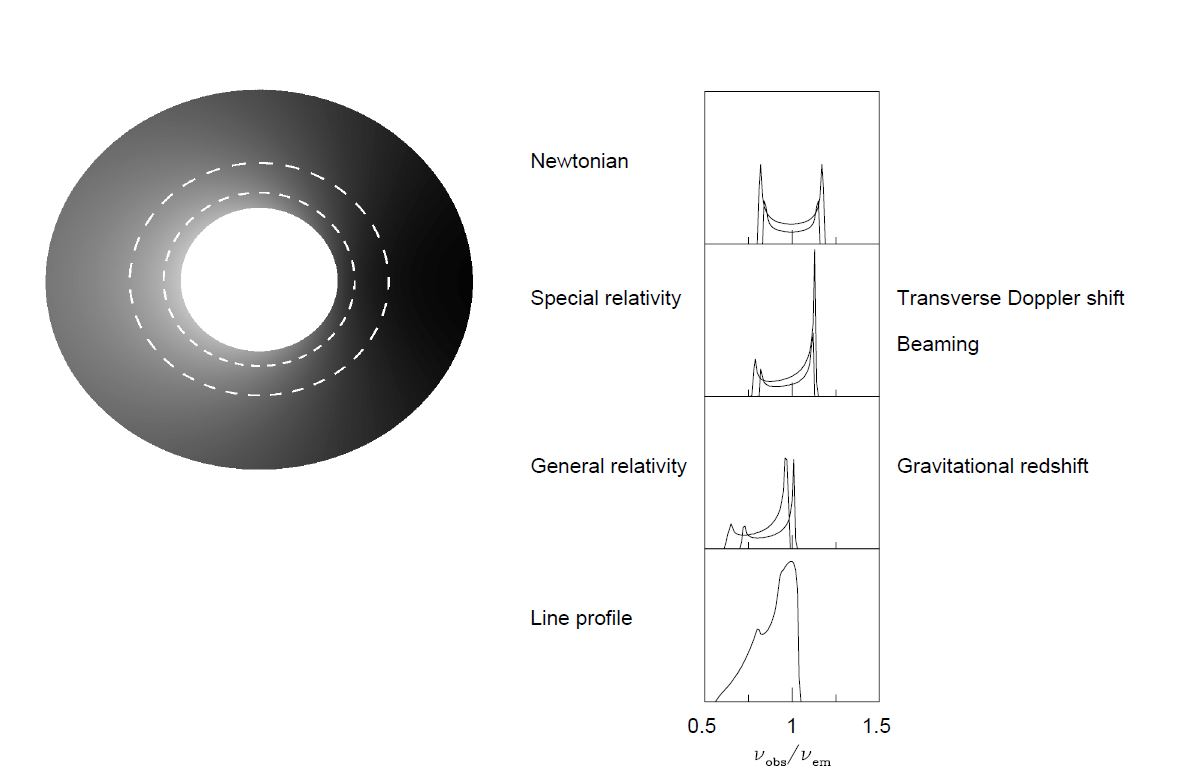
\includegraphics[keepaspectratio]{images/ShapeOfIronLine.jpg}}

}

\caption{The profile of the broad iron line, image credit to Fabian
(2000)~{[}1{]}.}

\end{figure}%

Soft Comptonisation (multiple inverse Compton scattering by hot thermal
electrons) occurs giving a power law X-ray spectrum. Flares from active
or flaring regions irradiate the accretion disk forming a ``reflection''
component in the spectrum.

\begin{figure}[H]

{\centering 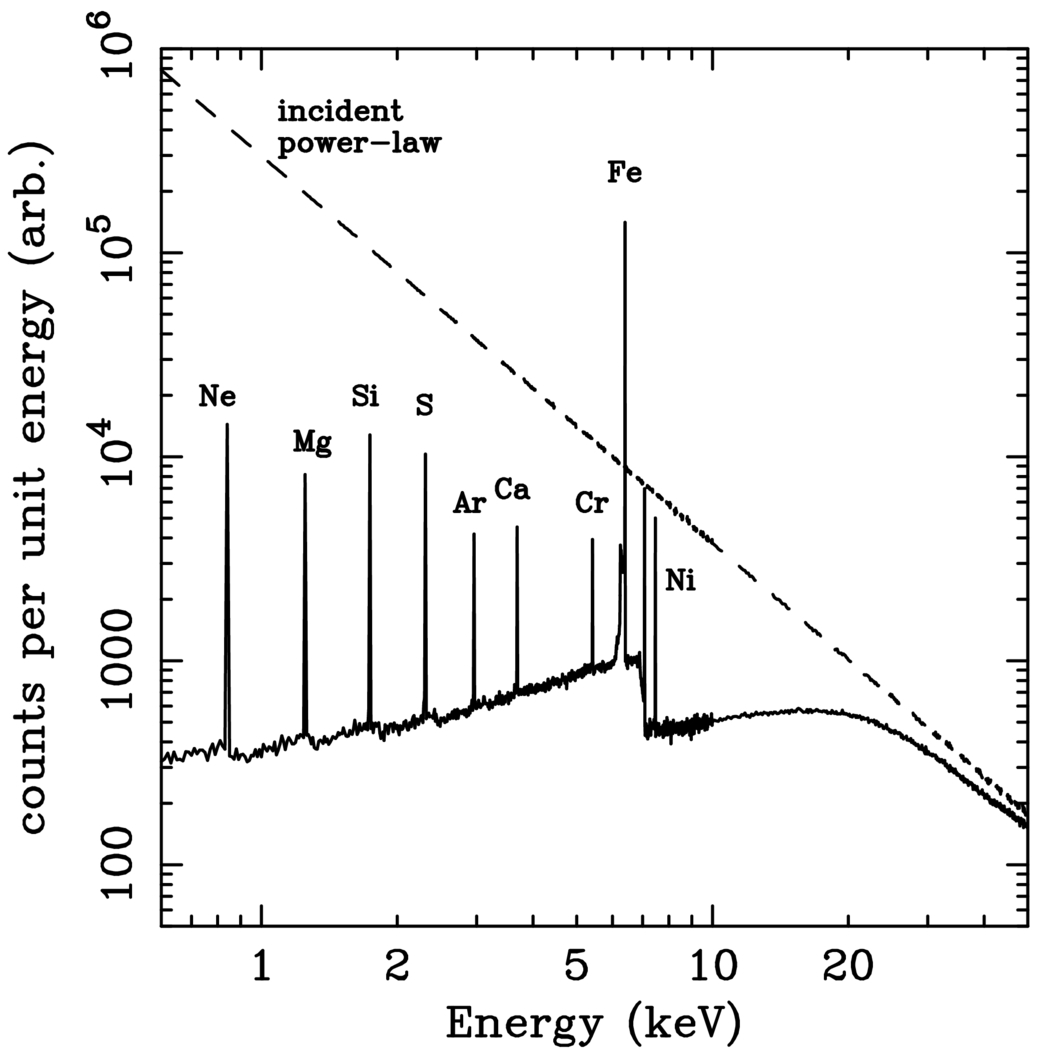
\includegraphics[width=10cm,height=\textheight,keepaspectratio]{images/ReflectionSpectrum.jpg}

}

\caption{Reflection spectrum from a Monte Carlo simulation of an
illuminated slab. The dashed line is the incident continuum and the
solid line shows the reflected spectrum. Image credit Reynolds
(1996)~{[}1{]}}

\end{figure}%

The iron line is produced when one of the two K-shell electrons is
ejected following absorption of an X-ray, the threshold for neutral iron
is 7.1 keV. The resultant state can decay through the dropping of an
L-shell electron into the K-shell, releasing 6.4 keV as either an
emission line photon (34\%) or an Auger electron (66\%). Ionised iron
has a photoelectric threshold and the K\(\alpha\) of higher energy. The
strength of the iron line is measured in terms of its equivalent width.

\begin{tcolorbox}[enhanced jigsaw, arc=.35mm, bottomrule=.15mm, bottomtitle=1mm, breakable, colback=white, colbacktitle=quarto-callout-note-color!10!white, colframe=quarto-callout-note-color-frame, coltitle=black, left=2mm, leftrule=.75mm, opacityback=0, opacitybacktitle=0.6, rightrule=.15mm, title=\textcolor{quarto-callout-note-color}{\faInfo}\hspace{0.5em}{Equivalent Width}, titlerule=0mm, toprule=.15mm, toptitle=1mm]

The equivalent width of a spectral line is the width of the rectangle
which has the same area as that between the line and the continuum
level.

\begin{figure}[H]

{\centering 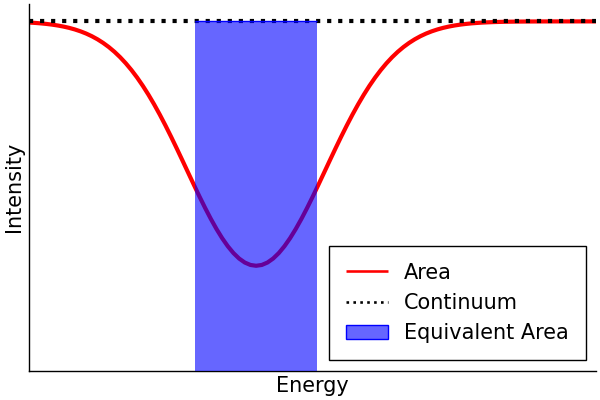
\includegraphics[width=10cm,height=\textheight,keepaspectratio]{images/EquivalentWidth.png}

}

\caption{A diagram indicating the equivalent width. The width of the
rectangle is the equivalent width.}

\end{figure}%

\end{tcolorbox}

The equivalent width is a function of the geometry of the accretion
disk, the elemental abundances, the inclination angle, and the
ionisation state.

\begin{tcolorbox}[enhanced jigsaw, arc=.35mm, bottomrule=.15mm, bottomtitle=1mm, breakable, colback=white, colbacktitle=quarto-callout-important-color!10!white, colframe=quarto-callout-important-color-frame, coltitle=black, left=2mm, leftrule=.75mm, opacityback=0, opacitybacktitle=0.6, rightrule=.15mm, title=\textcolor{quarto-callout-important-color}{\faExclamation}\hspace{0.5em}{Key Points}, titlerule=0mm, toprule=.15mm, toptitle=1mm]

\begin{itemize}
\tightlist
\item
  \textbf{X-ray Continuum}: The hard X-ray continuum in AGNs and GBHCs
  is thought to be from active/flaring regions in the corona. Thermal
  electrons multiply inverse Compton scatter optical and UV photons from
  the disk to X-ray energies. A hard X-ray power law results and
  irradiates the accretion disk to produce a reflection component.
\item
  \textbf{Reflection Component}: The reflection component causes the
  spectrum to flatten above 10 keV as Compton recoil reduces the
  backscattered flux and results in a strong fluorescent iron line at
  \(\sim 6.4\) keV. The energy and strength of this line depends on iron
  abundance, inclination of the disk, and its ionisation state. A strong
  iron absorption edge may also be present from an ionised disk.
\item
  \textbf{Iron Line Profile}: Doppler shifts, relativistic broadening
  and gravitational redshifting give the broad and skewed line profile.
  As the line comes from the innermost regions, these effects are very
  pronounced and may be used to determine the black hole spin and
  inclination angle of the accretion disk. In most Seyfert 1 galaxies,
  the disk is inclined at around 30\(^\circ\), consistent with the
  standard model.
\item
  \textbf{Observations}: The iron line was first clearly detected by
  Ginga and a line profile subsequently resolved by ASCA confirmed the
  broad and skewed shape expected from an accretion disk around a
  Schwarzschild black hole. RXTE has been used to study the line and
  continuum variability on shorter timescales, with reduced energy
  resolution.
\item
  \textbf{Black Hole Spin}: The radius of the ISCO decreases with spin.
  Since the line profile is sensitive to the innermost radius of
  fluorescent emission this may be used to estimate the black hole, with
  some astrophysical assumptions. With present time-averaged
  observations such measurements may be ambiguous as alternative models
  with different values for the spin may produce identical line
  profiles.
\item
  \textbf{Alternative Models for the Production of the Broad Iron Line}:
  Alternative models that do not require an accretion disk appear to
  fail, in particular the line width cannot be entirely due to
  Comptonisation. Hybrid models in which the Comptonisation and
  Doppler/gravitational effects produce the profile are heavily
  constrained.
\item
  \textbf{Variability}: Rapid X-ray continuum variability is observed in
  most AGNs, and the iron line is expected to vary in response to this
  with short time lag. Whilst these timescales are too short to be
  probed presently, significant and complex iron line variability has
  been observed. Often the line flux is seen to remain constant whilst
  the continuum changes, and there appears to be an anticorrelation
  between the reflected fraction and the equivalent width. In another
  study the reflected fraction and the photon index of the power law are
  correlated for individual objects and between different ones. These
  need to be explained as they appear contrary to our simple model of
  reflection. Flux correlated changes in the ionisation state of the
  disk may explain some of these facts.
\item
  \textbf{Reverberation Mapping}: The rapid variability is associated
  with activation of new flares in the corona above the accretion disk.
  X-ray reverberation mapping uses observations of the iron line
  response to sudden changes in the continuum to study the accretion
  disk and black hole. This may be used to determine the geometry of the
  X-ray emission and the black hole spin and mass.
\item
  \textbf{Other Classes of Object} Iron lines are observed in quasars,
  LLAGNs, radio-loud AGNs, and GBHCs. Quasars have the iron line
  decrease with increasing luminosity which may be due to the more
  luminous sources accreting closer to the Eddington limit being more
  highly ionised. Observations in LLAGNs may determine whether the
  accretion with low rates is an advection‐dominated accretion flow or a
  thin disk. Weak lines have been observed suggesting that their low
  accretion rate flows are thin disks rather than optically thick ADAFs.
  THe broad iron lines and reflection humps are weak or absent perhaps
  because the reflection signature is swamped by a beamed continuum.
  GBHCs show smeared absorption and emission features in the reflection
  spectra, and there is a debate as to the precise nature of the
  accretion flow within a few tens of Schwarzschild radii.
\end{itemize}

\end{tcolorbox}

\begin{center}\rule{0.5\linewidth}{0.5pt}\end{center}

\bookmarksetup{startatroot}

\chapter{Initial Gradus Testing}\label{initial-gradus-testing}

\begin{center}\rule{0.5\linewidth}{0.5pt}\end{center}

The below details initial experimentation with \texttt{Gradus.jl}. The
code block below renders an image of a black hole with a thick accretion
disk. Colour denotes the redshift of a given region on the disk.

\begin{Shaded}
\begin{Highlighting}[]
\ImportTok{using} \BuiltInTok{Gradus}
\ImportTok{using} \BuiltInTok{Plots}

\CommentTok{\# Function defining the cross section of the disk}
\KeywordTok{function} \FunctionTok{discCrossSection}\NormalTok{(x)}
\NormalTok{    centre }\OperatorTok{=} \FloatTok{8}
\NormalTok{    radius }\OperatorTok{=} \FloatTok{3}

    \ControlFlowTok{if}\NormalTok{ (x }\OperatorTok{\textless{}}\NormalTok{ centre }\OperatorTok{{-}}\NormalTok{ radius) }\OperatorTok{||}\NormalTok{ (radius }\OperatorTok{+}\NormalTok{ centre }\OperatorTok{\textless{}}\NormalTok{ x)}
        \FunctionTok{zero}\NormalTok{(x)}
    \ControlFlowTok{else} 
\NormalTok{        r }\OperatorTok{=}\NormalTok{ x }\OperatorTok{{-}}\NormalTok{ centre}
        \FloatTok{0.5}\NormalTok{(}\FunctionTok{sqrt}\NormalTok{(radius}\OperatorTok{\^{}}\FloatTok{2} \OperatorTok{{-}}\NormalTok{ r}\OperatorTok{\^{}}\FloatTok{2}\NormalTok{) }\OperatorTok{+}\NormalTok{ (}\FloatTok{0.5}\FunctionTok{sin}\NormalTok{(}\FloatTok{3}\NormalTok{x)))}
    \ControlFlowTok{end}
\KeywordTok{end}

\CommentTok{\# Metric Parameters}
\NormalTok{M }\OperatorTok{=} \FloatTok{1.0}     \CommentTok{\# Mass}
\NormalTok{a }\OperatorTok{=} \FloatTok{0.7}     \CommentTok{\# Black hole spin}
\NormalTok{α}\FloatTok{13} \OperatorTok{=} \FloatTok{0.0}   
\NormalTok{α}\FloatTok{22} \OperatorTok{=} \FloatTok{0.0}
\NormalTok{α}\FloatTok{52} \OperatorTok{=} \FloatTok{0.0}
\NormalTok{ϵ}\FloatTok{3} \OperatorTok{=} \FloatTok{0.0}
\NormalTok{i }\OperatorTok{=} \FunctionTok{deg2rad}\NormalTok{(}\FloatTok{70}\NormalTok{) }\CommentTok{\# Inclination}

\CommentTok{\# Instantiating the metric}
\NormalTok{m }\OperatorTok{=} \FunctionTok{JohannsenMetric}\NormalTok{(M, a, α}\FloatTok{13}\NormalTok{, α}\FloatTok{22}\NormalTok{, α}\FloatTok{52}\NormalTok{, ϵ}\FloatTok{3}\NormalTok{)}

\CommentTok{\# Position of the observer}
\CommentTok{\# (x[1], Distance, Inclination, x[4])}
\NormalTok{x }\OperatorTok{=} \FunctionTok{SVector}\NormalTok{(}\FloatTok{0.0}\NormalTok{, }\FloatTok{1000.0}\NormalTok{, i, }\FloatTok{0.0}\NormalTok{)}

\CommentTok{\# Maximum affine time, parameterises the solution}
\CommentTok{\# λ\_max \textasciitilde{} 2*x[2]}
\NormalTok{λ\_max }\OperatorTok{=} \FloatTok{2000.0}

\CommentTok{\# Setting up impact parameters}
\NormalTok{α }\OperatorTok{=} \FunctionTok{range}\NormalTok{(}\OperatorTok{{-}}\FloatTok{10.0}\NormalTok{, }\FloatTok{10.0}\NormalTok{, }\FloatTok{100}\NormalTok{)}
\NormalTok{β }\OperatorTok{=} \FunctionTok{range}\NormalTok{(}\OperatorTok{{-}}\FloatTok{10.0}\NormalTok{, }\FloatTok{10.0}\NormalTok{, }\FloatTok{100}\NormalTok{)}

\CommentTok{\# Getting an array of velocities from the impact parameters}
\NormalTok{vs }\OperatorTok{=} \FunctionTok{vec}\NormalTok{([}\FunctionTok{map\_impact\_parameters}\NormalTok{(m, x, a, b) for a }\KeywordTok{in}\NormalTok{ α, b }\KeywordTok{in}\NormalTok{ β])}
\NormalTok{xs }\OperatorTok{=} \FunctionTok{fill}\NormalTok{(x, }\FunctionTok{size}\NormalTok{(vs))}

\CommentTok{\# Generating solutions}
\NormalTok{sols }\OperatorTok{=} \FunctionTok{tracegeodesics}\NormalTok{(m, xs, vs, λ\_max, save\_on }\OperatorTok{=} \ConstantTok{false}\NormalTok{)}

\CommentTok{\# Generating points and reshaping to be the same shape as the image}
\NormalTok{points }\OperatorTok{=} \FunctionTok{unpack\_solution}\NormalTok{.(sols.u)}
\NormalTok{points }\OperatorTok{=} \FunctionTok{reshape}\NormalTok{(points, (}\FloatTok{100}\NormalTok{, }\FloatTok{100}\NormalTok{))}

\CommentTok{\# Redshift point function}
\NormalTok{redshift }\OperatorTok{=}\NormalTok{ ConstPointFunctions.}\FunctionTok{redshift}\NormalTok{(m, x)}
\NormalTok{redshiftGeometry }\OperatorTok{=}\NormalTok{ redshift }\OperatorTok{∘}\NormalTok{ ConstPointFunctions.}\FunctionTok{filter\_intersected}\NormalTok{()}

\CommentTok{\# Disc}
\NormalTok{d }\OperatorTok{=} \FunctionTok{ThickDisc}\NormalTok{(r }\OperatorTok{{-}\textgreater{}} \FunctionTok{discCrossSection}\NormalTok{(r))}

\CommentTok{\# this function returns the impact parameter axes}
\NormalTok{α, β, image }\OperatorTok{=} \FunctionTok{rendergeodesics}\NormalTok{(}
\NormalTok{    m, x, d, λ\_max, pf }\OperatorTok{=}\NormalTok{ redshiftGeometry,}
    \CommentTok{\# image parameters}
\NormalTok{    image\_width }\OperatorTok{=} \FloatTok{200}\NormalTok{, image\_height }\OperatorTok{=} \FloatTok{150}\NormalTok{,}
    \CommentTok{\# the "zoom" {-}{-} use the impact parameter axes}
\NormalTok{    αlims }\OperatorTok{=}\NormalTok{ (}\OperatorTok{{-}}\FloatTok{20}\NormalTok{, }\FloatTok{20}\NormalTok{), βlims }\OperatorTok{=}\NormalTok{ (}\OperatorTok{{-}}\FloatTok{15}\NormalTok{, }\FloatTok{15}\NormalTok{), verbose }\OperatorTok{=} \ConstantTok{false}
\NormalTok{)}

\FunctionTok{heatmap}\NormalTok{(α, β, image, aspect\_ratio }\OperatorTok{=} \FloatTok{1}\NormalTok{)}
\end{Highlighting}
\end{Shaded}

\begin{figure}[H]

{\centering \pandocbounded{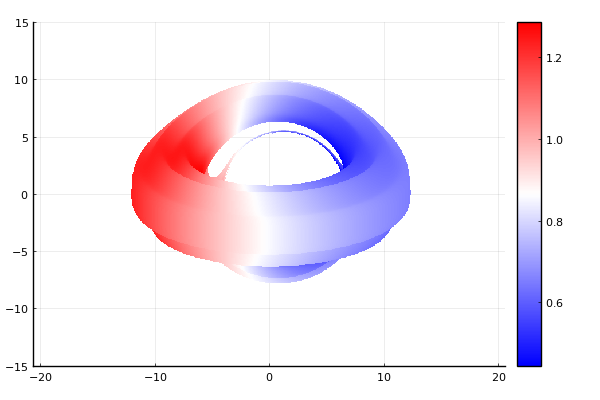
\includegraphics[keepaspectratio]{images/render.png}}

}

\caption{The first render produced.}

\end{figure}%

Once familiarity was gained with the basics of \texttt{Gradus.jl} the
line profile functionality was utilised through the following function.

\begin{Shaded}
\begin{Highlighting}[]
\KeywordTok{function} \FunctionTok{computeLineProfile}\NormalTok{(m, i, height, bins }\OperatorTok{=} \FunctionTok{range}\NormalTok{(}\FloatTok{0.0}\NormalTok{, }\FloatTok{1.5}\NormalTok{, }\FloatTok{180}\NormalTok{))}
    \CommentTok{\# Position of the observer}
    \CommentTok{\# (x[1], Distance, Inclination, x[4])}
\NormalTok{    x }\OperatorTok{=} \FunctionTok{SVector}\NormalTok{(}\FloatTok{0.0}\NormalTok{, }\FloatTok{10000.0}\NormalTok{, i, }\FloatTok{0.0}\NormalTok{)}

    \CommentTok{\# Disk}
\NormalTok{    d }\OperatorTok{=} \FunctionTok{ThinDisc}\NormalTok{(}\FloatTok{0.0}\NormalTok{, }\ConstantTok{Inf}\NormalTok{)}

    \CommentTok{\# Setting up the model and profile}
\NormalTok{    model }\OperatorTok{=} \FunctionTok{LampPostModel}\NormalTok{(h }\OperatorTok{=}\NormalTok{ height)}
\NormalTok{    profile }\OperatorTok{=} \FunctionTok{emissivity\_profile}\NormalTok{(m, d, model)}

    \CommentTok{\# Computing the line profile}
\NormalTok{    bins, flux }\OperatorTok{=} \FunctionTok{lineprofile}\NormalTok{(m, x, d, profile; bins}\OperatorTok{=}\NormalTok{bins, verbose}\OperatorTok{=}\ConstantTok{true}\NormalTok{)}

    \ControlFlowTok{return}\NormalTok{ bins, flux}
\KeywordTok{end}
\end{Highlighting}
\end{Shaded}

This will allow for the investigation of the free parameters for the
Johannsen metric; \(\alpha_{13}\), \(\alpha_{22}\), \(\alpha_{52}\), and
\(\epsilon_3\). A lamppost corona model is used with variable height
\texttt{h}. An example of the effect of varying the height of this
corona is shown below.

\begin{figure}[H]

{\centering \pandocbounded{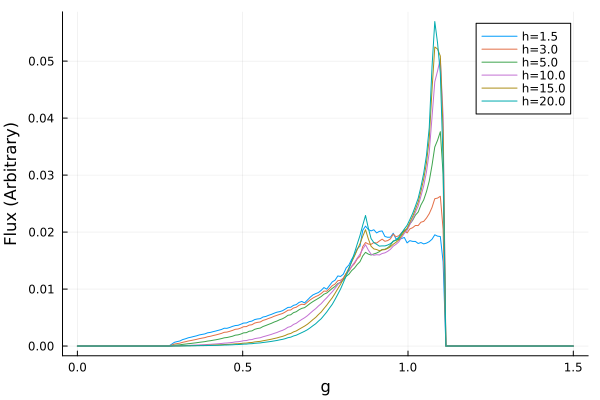
\includegraphics[keepaspectratio]{images/InitialHVariation.png}}

}

\caption{Initial variations of the height of the lamppost corona.}

\end{figure}%

Following initial experimentation the two functions above were
integrated together for efficient investigation. The two free parameters
that will be the focus of this investigation are \(\alpha_{13}\) and
\(\epsilon_3\). Examples of the effects of these parameters on the
emission lines are shown below

\pandocbounded{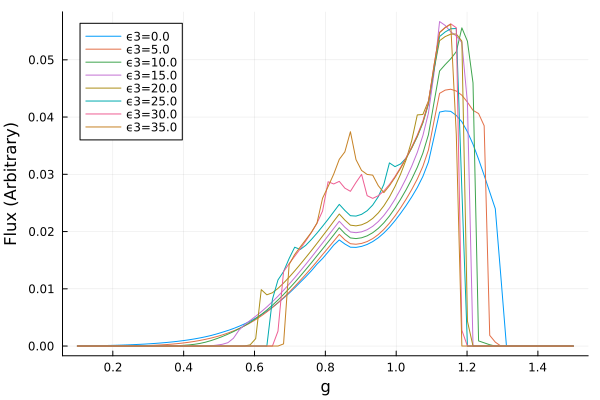
\includegraphics[keepaspectratio]{images/epsilon3vars.png}}

\begin{figure}[H]

{\centering \pandocbounded{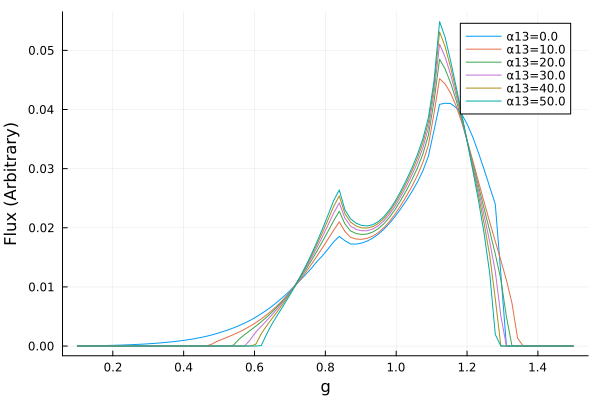
\includegraphics[keepaspectratio]{images/alpha13vars.png}}

}

\caption{Initial variations of \(\alpha_{13}\) and \(\epsilon_3\)}

\end{figure}%

It can be seen that \(\alpha_{13}\) has a very smooth, almost linear
effect on the shape of the line, while \(\epsilon_3\) is much more
chaotic, particularly for \(\epsilon_3>25\).

\bookmarksetup{startatroot}

\chapter{Parameter Space
Investigations}\label{parameter-space-investigations}

\begin{center}\rule{0.5\linewidth}{0.5pt}\end{center}

Code was set up to easily run several variations to the model which will
allow for the investigation of the parameter space. A thin disk
accretion model and a lamppost corona were used. It was set up such that
for a given configuration of \(h\), \(a\), \(i\), \(\epsilon_3\), and
\(\alpha_{13}\) the line profile would be calculated and an image of the
accretion disk produced and plotted together.

\section{\texorpdfstring{Ruling out \(\alpha_{22}\) and
\(\alpha_{52}\)}{Ruling out \textbackslash alpha\_\{22\} and \textbackslash alpha\_\{52\}}}\label{ruling-out-alpha_22-and-alpha_52}

Before exploring the 5D parameter space, tests were ran on both
\(\alpha_{22}\) and \(\alpha_{52}\) such that their effects could be
noted, should they be useful in the future.

\begin{figure}

\centering{

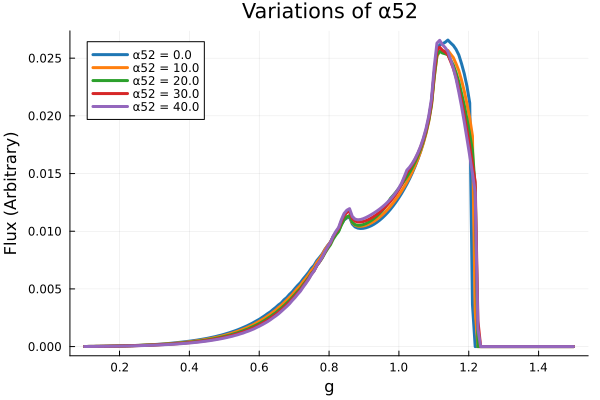
\includegraphics[width=0.7\linewidth,height=\textheight,keepaspectratio]{images/alpha52.png}

}

\caption{\label{fig-alpha52}The resultant line profile from varying
\(\alpha_{52}\) between 0 and 40. A value of 50 did not successfully
compute suggesting an upper limit on this parameter.}

\end{figure}%

Varying \(\alpha_{52}\) showed near random, and near zero effect on the
line and will thus be disregarded for this investigation. Varying
\(\alpha_{22}\) often failed to compute and will thus similarly be
disregarded for this investigation.

\section{Exploring the 5-dimensional parameter
space}\label{exploring-the-5-dimensional-parameter-space}

Before varying the parameters it was necessary to determine the limits
for useful variations. The spin is fundamentally limited to be
\(|a|<|M|\) and will thus be varied between 0 and 1. The ranges and
default values for the parameter space are tabulated in
Table~\ref{tbl-defaultsRanges}.

\begin{longtable}[]{@{}llll@{}}
\caption{The ranges and default values for the parameter
space.}\label{tbl-defaultsRanges}\tabularnewline
\toprule\noalign{}
Parameter & Minimum & Maximum & Default \\
\midrule\noalign{}
\endfirsthead
\toprule\noalign{}
Parameter & Minimum & Maximum & Default \\
\midrule\noalign{}
\endhead
\bottomrule\noalign{}
\endlastfoot
\(\alpha_{13}\) & 0.0 & 50.0 & 0.0 \\
\(\epsilon_{3}\) & 0.0 & 30.0 & 0.0 \\
\(a\) & 0.0 & 1.0 & 0.998 \\
\(h\) & \(R_\text{ISCO}\) & 30 \(R_G\) & 10 \(R_G\) \\
\(i\) & 0.0\(\degree\) & 90.0\(\degree\) & 60\(\degree\) \\
\end{longtable}

\subsection{Line profiles}\label{line-profiles}

\begin{figure}

\begin{minipage}[t]{0.50\linewidth}

\begin{figure}[H]

\centering{

\pandocbounded{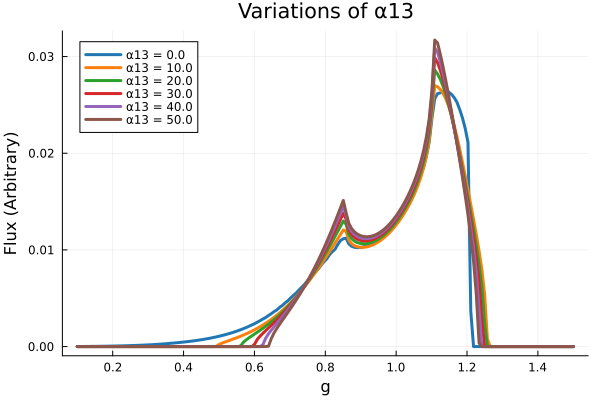
\includegraphics[keepaspectratio]{images/alpha13.png}}

}

\caption{\label{fig-alpha13}The line profiles resultant from varying
\(\alpha_{13}\) between 0 and 50.}

\end{figure}%

\end{minipage}%
%
\begin{minipage}[t]{0.50\linewidth}

\begin{figure}[H]

\centering{

\pandocbounded{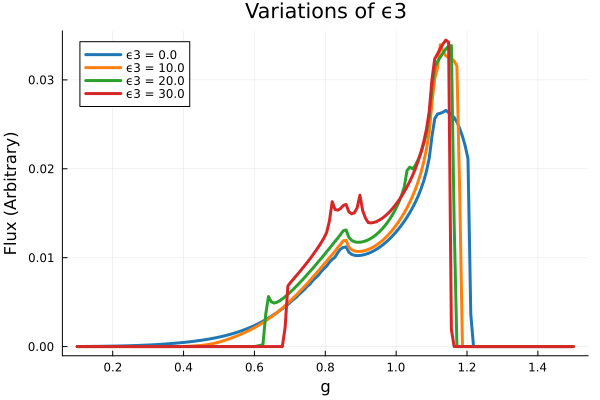
\includegraphics[keepaspectratio]{images/epsilon3.png}}

}

\caption{\label{fig-epsilon3}The line profiles resultant from varying
\(\epsilon_{3}\) between 0 and 30. Values of 40 and 50 were tested
however caused an error, there must be an upper bound on the allowed
values of this parameter.}

\end{figure}%

\end{minipage}%
\newline
\begin{minipage}[t]{0.50\linewidth}

\begin{figure}[H]

\centering{

\pandocbounded{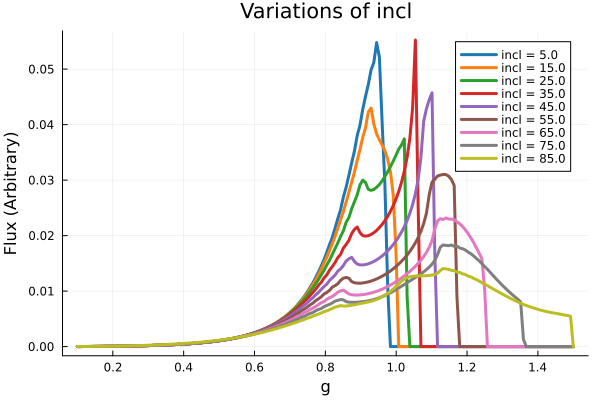
\includegraphics[keepaspectratio]{images/inclination.png}}

}

\caption{\label{fig-inclination}The line profiles resultant from varying
the inclination between 5 and 85 degrees.}

\end{figure}%

\end{minipage}%
%
\begin{minipage}[t]{0.50\linewidth}

\begin{figure}[H]

\centering{

\pandocbounded{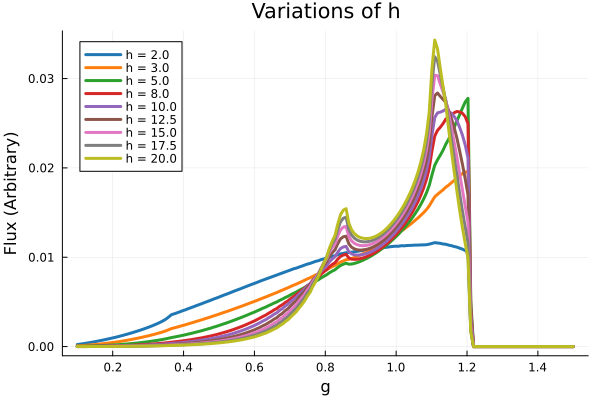
\includegraphics[keepaspectratio]{images/coronaHeight.png}}

}

\caption{\label{fig-coronaHeight}The line profiles resultant from
varying \(h\) between 5 and 30 gravitational radii.}

\end{figure}%

\end{minipage}%
\newline
\begin{minipage}[t]{0.50\linewidth}

\begin{figure}[H]

\centering{

\pandocbounded{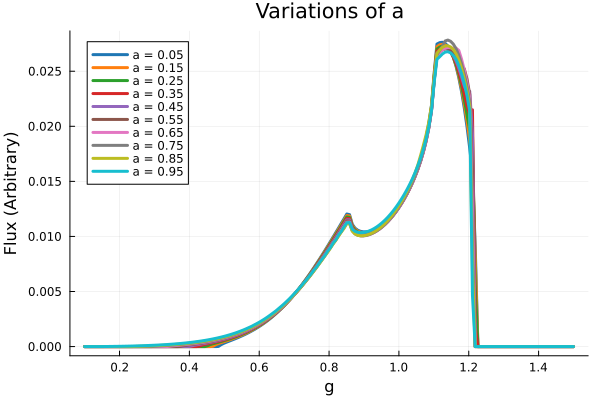
\includegraphics[keepaspectratio]{images/spin.png}}

}

\caption{\label{fig-spin}The line profiles resultant from varying \(a\)
between 5 and 95\% of \(M(=1)\).}

\end{figure}%

\end{minipage}%

\end{figure}%

\begin{itemize}
\tightlist
\item
  Figure~\ref{fig-alpha13} shows that increasing the free parameter
  \(\alpha_{13}\) sharpens the two peaks of the line, increases the
  maximum flux, and makes it more narrow.
\item
  Figure~\ref{fig-epsilon3} shows that increasing the free parameter
  \(\epsilon_{3}\) similarly increases the maximum flux, however the
  resultant profile is much more noisy. While \(\alpha_{13}\) provided
  sharp peaks, \(\epsilon_{3}\) provided broader peaks, particularly in
  the shorter one.
\item
  Figure~\ref{fig-inclination} shows that increasing the inclination
  smoothes out the line profile and shifts the peak to higher energies.
  The line is broadened significantly.
\item
  Figure~\ref{fig-coronaHeight} shows that increasing the corona height
  makes the line profile sharper, increases the maximum flux, and shifts
  the maximum to slightly lower energies.
\item
  Figure~\ref{fig-spin} shows that the spin had the least prominent
  impact on the profile of the line, seeming to only slightly decrease
  the height of the peaks with increasing spin. This may be an effect of
  the small range of spins available. It may therefore be informative to
  investigate this further by increasing the mass, using different
  corona heights, or varying the inclination.
\end{itemize}

\subsection{Redshift Image Renders}\label{redshift-image-renders}

Alongside the line profiles, images of the accretion disk were rendered
with a colourmap denoting the redshift of light from a given part of the
disk. The corona height was not varied here as it did not impact the
render.

\begin{figure}

\centering{

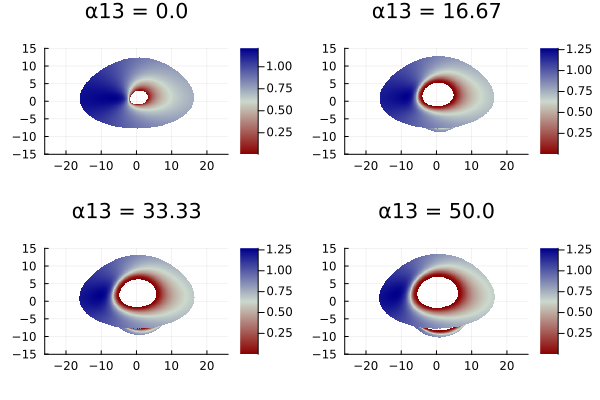
\includegraphics[width=0.8\linewidth,height=\textheight,keepaspectratio]{images/alpha13Render.png}

}

\caption{\label{fig-alpha13Render}The effect of \(\alpha_{13}\) on the
accretion disk render. The ISCO appears to grow with \(\alpha_{13}\)}

\end{figure}%

\begin{figure}

\centering{

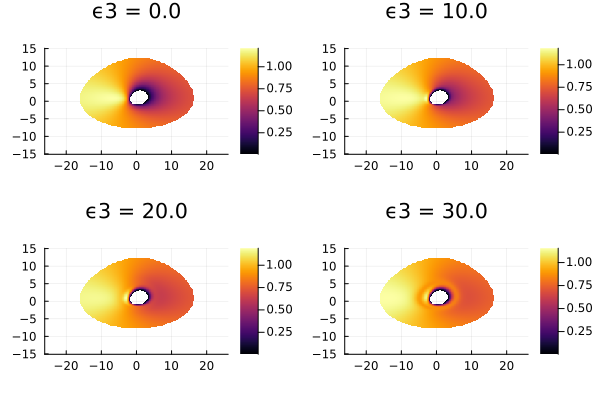
\includegraphics[width=0.8\linewidth,height=\textheight,keepaspectratio]{images/epsilon3Render.png}

}

\caption{\label{fig-epsilon3Render}The effect of \(\epsilon_3\) on the
redshift image. The shape of the disk does not change but the redshift
profile does, particularly in the shrinking of the blueshift region, and
an overall decrease in the degree of redshifting.}

\end{figure}%

\begin{figure}

\centering{

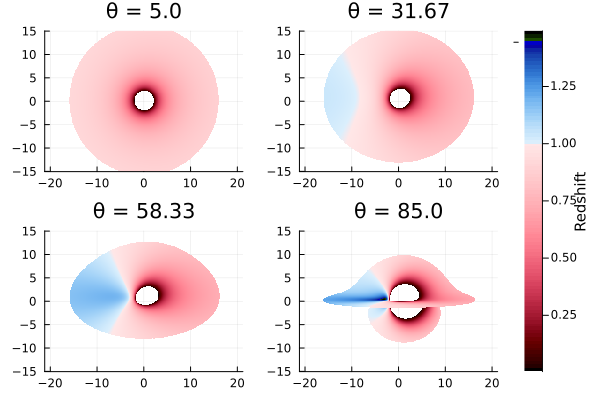
\includegraphics[width=0.8\linewidth,height=\textheight,keepaspectratio]{images/inclRender.png}

}

\caption{\label{fig-inclRender}The effect of inclination on the redshift
image. The redshift becomes more apparent as the inclination increases
and the disk becomes edge on. This agrees with the observed line profile
trend of energy increasing with inclination as the effects of doppler
shifting become more apparent with increasing energy.}

\end{figure}%

\begin{figure}

\centering{

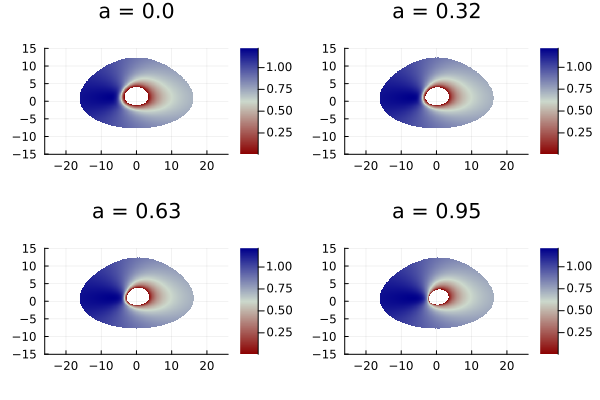
\includegraphics[width=0.8\linewidth,height=\textheight,keepaspectratio]{images/spinRender.png}

}

\caption{\label{fig-spinRender}The effect of black hole spin on the
redshift image. The ISCO appears to shrink.}

\end{figure}%

Some of the parameters appeared to change the radius of the ISCO. This
was investigated by explicitly finding the ISCO, as tabulated below.

{\def\LTcaptype{none} % do not increment counter
\begin{longtable}[]{@{}lll@{}}
\toprule\noalign{}
Parameter & Value & ISCO (\(R_G\)) \\
\midrule\noalign{}
\endhead
\bottomrule\noalign{}
\endlastfoot
\(\alpha_{13}\) & 0.00 & 1.24 \\
& 16.67 & 8.62 \\
& 33.33 & 11.70 \\
& 50.00 & 14.03 \\
\(\epsilon_3\) & 0.00 & 1.24 \\
& 10.00 & 2.36 \\
& 20.00 & 2.90 \\
& 30.00 & 3.51 \\
\(a\) & 0.00 & 6.00 \\
& 0.32 & 4.92 \\
& 0.63 & 3.68 \\
& 0.95 & 1.94 \\
\end{longtable}
}

The ISCO is proportional to both \(\alpha_{13}\) and \(\epsilon_3\), and
inversely proportional to the spin.

\section{Summary}\label{summary}

\begin{tcolorbox}[enhanced jigsaw, arc=.35mm, bottomrule=.15mm, bottomtitle=1mm, breakable, colback=white, colbacktitle=quarto-callout-important-color!10!white, colframe=quarto-callout-important-color-frame, coltitle=black, left=2mm, leftrule=.75mm, opacityback=0, opacitybacktitle=0.6, rightrule=.15mm, title=\textcolor{quarto-callout-important-color}{\faExclamation}\hspace{0.5em}{Summary}, titlerule=0mm, toprule=.15mm, toptitle=1mm]

\begin{itemize}
\tightlist
\item
  \(\alpha_{22}\) and \(\alpha_{52}\) had unpredictable or minimal
  effect on the line profile and rendered images so are therefore to be
  disregarded.
\item
  \(a\): Increasing the spin appears to shrink the ISCO of the accretion
  disk. Its effect on the line profile is less obvious, it appears to
  decrease the flux slightly but is otherwise negligible.
\item
  \(h\): Increasing the corona height makes the line profile sharper and
  increases the peak flux, while decreasing the energy of the peak. It
  has no effect on the renders.
\item
  \(\theta\): Increasing the inclination (where 0 degrees has the
  accretion disk face-on) smoothes out the line profile and increases
  the peak energy. The effect of redshift becomes more apparent with
  increased inclination.
\item
  \(\alpha_{13}\): Increasing \(\alpha_{13}\) appears to increase the
  radius of the ISCO and make the line profile sharper.
\item
  \(\epsilon_3\): Increasing \(\epsilon_3\) increases the height of the
  line profile, and makes it more chaotic.
\item
  The ISCO is proportional to both \(\alpha_{13}\) and \(\epsilon_3\),
  and inversely proportional to the spin.
\end{itemize}

\end{tcolorbox}

\section{Code Specifics}\label{code-specifics}

The workhorse of the parameter investigations was the utility function
\texttt{JohannsenParamVar} which sets up the metric and observer
position and then calls either \texttt{ComputeLineProfile} or
\texttt{RenderImage}. This utility function was made versatile using
keyword arguments allowing for different methods to be called within it.
This was then wrapped in \texttt{ParamLoop} which took the index (the
variable to be looped through) and a set of values to call
\texttt{JohannsenParamVar} for.

To maximise readablity of the redshift images, a custom colormap is made
through \texttt{RedshiftColormap} which gives red for any values \(<1\),
blue for those \(>1\), and white for those \(=1\). This gave the images
seen in
Figure~\ref{fig-alpha13Render}, \ref{fig-epsilon3Render}, \ref{fig-inclRender}, \ref{fig-spinRender}.

\bookmarksetup{startatroot}

\chapter{Fitting Spectral Lines}\label{fitting-spectral-lines}

With the parameter space explored, it was useful to setup the
architecture for fitting the model to spectral data. This was done using
\texttt{SpectralFitting.jl} and defining a custom model using Gradus
which fits the following parameters:

{\def\LTcaptype{none} % do not increment counter
\begin{longtable}[]{@{}ll@{}}
\toprule\noalign{}
Parameter & Meaning \\
\midrule\noalign{}
\endhead
\bottomrule\noalign{}
\endlastfoot
\texttt{K} & Normalisation \\
\texttt{h} & Corona Height \\
\texttt{E} & Line Energy \\
\texttt{R\_in} & Inner Radius \\
\texttt{R\_out} & Outer Radius \\
\texttt{θ} & Inclination \\
\texttt{a} & Spin \\
\texttt{α13} & \(\alpha_{13}\) Parameter \\
\texttt{ϵ3} & \(\epsilon_{3}\) Parameter \\
\end{longtable}
}

The architecture of this model was heavily based upon previous work on
\href{https://github.com/phajy/DiscAbsorption/blob/main/gradus-lamp-post.jl}{GitHub}.

The model is instantiated using the \texttt{LampPostJohannsen} utility
function. When called, the parameters are used to instantiate a
\texttt{JohannsenMetric}, observer position, \texttt{ThinDisc}, and an
emissivity profile. These are then used to compute the line profile as
previously done which is returned.

All fitting is handled by \texttt{SpectralFitting} through the Levenberg
Marquadt algorithm.

To test the implementation a line profile was computed and random noise
added to it. This was then passed through the fitting function. The
fitting process currently takes a long time and yields poor results so
more work is needed. Time was taken to streamline the functionality of
main2.jl via keyword arguments and general code cleanup.

\begin{figure}

\centering{

\pandocbounded{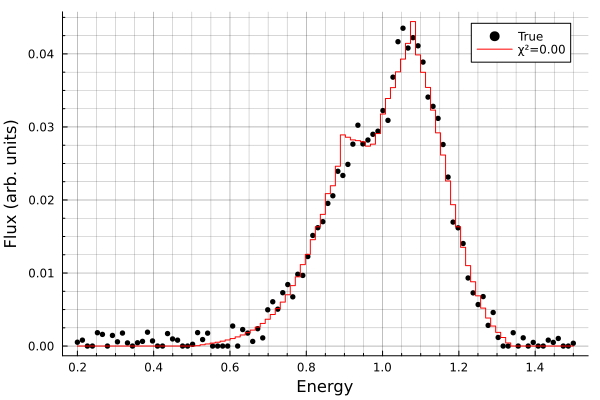
\includegraphics[keepaspectratio]{images/FirstFit.png}}

}

\caption{\label{fig-FirstFit}The first attempt at fitting to the noisy
simulated data. This fit took 67 iterations and 15.3 minutes to
complete.}

\end{figure}%

Upon fitting, the error
\texttt{Warning:\ No\ parameter\ uncertainty\ estimation\ due\ to\ error:\ LinearAlgebra.SingularException(3)}
occurs and therefore the fit is not currently quantified.

With the current errors present it was decided to attempt the fit on
actual data in order to determine whether they are a result of the data,
or the fitting algorithm.

\bookmarksetup{startatroot}

\chapter{Fitting to Data}\label{fitting-to-data}

Data from the NuSTAR (Nuclear Spectroscopic Telescope Array) spacecraft
~{[}2{]} was used, and the dataset used for testing was
\texttt{nu80402315002B01}. Data loading was handled by
\texttt{SpectralFitting.jl} through the \texttt{OGIPDataset} struct.
This takes the spectrum file as an argument and automatically pulls in
the background, \texttt{.arf}, and \texttt{.rmf} files to compute the
spectrum.

\section{Initial Results}\label{initial-results}

\begin{longtable}[]{@{}lllll@{}}
\caption{The ranges and default values for the parameter
space.}\label{tbl-InitialFit}\tabularnewline
\toprule\noalign{}
Model & Variable & Value & Error & \(\chi^2\) \\
\midrule\noalign{}
\endfirsthead
\toprule\noalign{}
Model & Variable & Value & Error & \(\chi^2\) \\
\midrule\noalign{}
\endhead
\bottomrule\noalign{}
\endlastfoot
Johannsen & \(a\) & 0.57 & 1.88 & 116.84 \\
& \(h\) & 50.00 & 8.77 & \\
& \(\theta\) & 58.24 & 4.93 & \\
& \(\alpha_{13}\) & 2.29 & 10.96 & \\
& \(\epsilon_3\) & 29.74 & 25.89 & \\
& \(K\) & 161.8 & 7.15 & \\
& \(E\) & 6.27 & 0.016 & \\
Kerr & \(a\) & 0.77 & 0.057 & 124.64 \\
& \(h\) & 50.0 & 2.75 & \\
& \(\theta\) & 55.44 & 2.67 & \\
& \(K\) & 162.0 & 7.07 & \\
& \(E\) & 6.27 & 0.014 & \\
\end{longtable}

\begin{figure}[H]

{\centering \pandocbounded{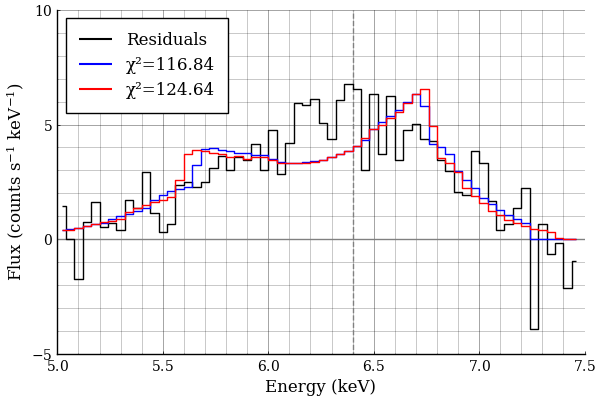
\includegraphics[keepaspectratio]{images/FirstDataFit.png}}

}

\caption{The first attempt at fitting to data. The Johannsen metric was
used to produce the blue line, and the Kerr metric was used to produce
the red. Neither fit was particularly good which may either be the
result of poor data, or a poor model.}

\end{figure}%

The NuSTAR datasets have two distinct spectra from each telescope, which
can be fit simultaneously, binding some of the parameters together. The
fitting code was thus adjusted to fit both datasets simultaneously while
binding all parameters other than the normalisation. The dataset
labelled ``nu80402315002'' was once again used.

\begin{figure}

\centering{

\pandocbounded{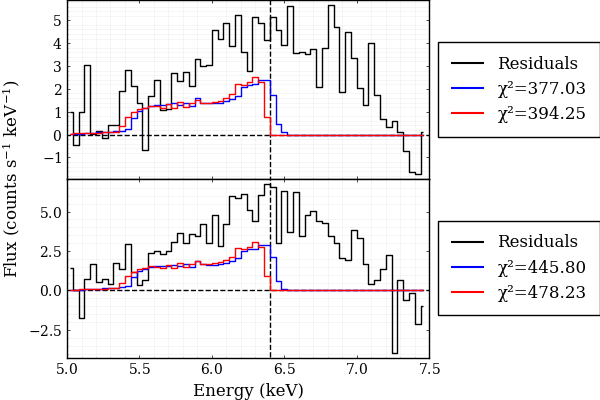
\includegraphics[keepaspectratio]{images/DualFit.png}}

}

\caption{\label{fig-DualFit}The fits to the nu80402315002 dataset. The
Johannsen fit is shown in blue, and the Kerr fit in red.}

\end{figure}%

It is evident from Figure~\ref{fig-DualFit} that the fitting process
needs refinement as the fits do not currently fit the data well, and
therefore drawing comparisons would be useless.

Following these experiments it was decided to fit a composite model of
\texttt{PowerLaw} + \texttt{LampPost}, with the latter being the line
profiles generated using either the Kerr or Johannsen metric through
\texttt{Gradus.jl}. The first attempt at this provided the plots below.

\begin{figure}[H]

{\centering \pandocbounded{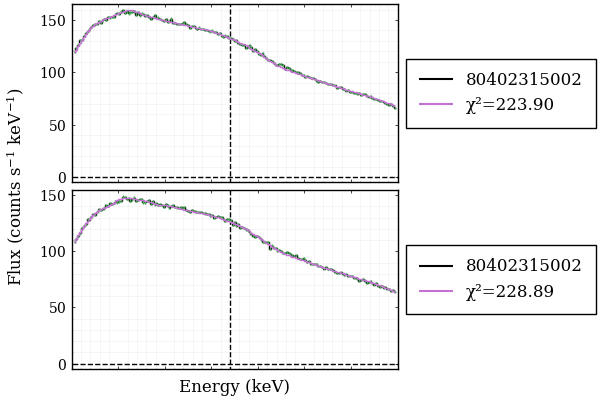
\includegraphics[keepaspectratio]{images/Johannsennu80402315002.png}}

}

\caption{The composite fit using the Johannsen metric.}

\end{figure}%

\begin{figure}[H]

{\centering \pandocbounded{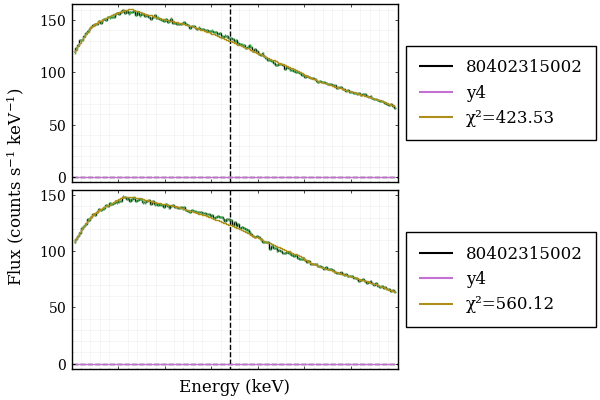
\includegraphics[keepaspectratio]{images/Kerrnu80402315002.png}}

}

\caption{The composite fit using the Kerr metric}

\end{figure}%

The inner and outer radii of the accretion disk were set constant at the
ISCO and 400 \(R_g\) respectively. The Johannsen metric currently seems
to yield a better fit, however this appears to be an effect of
parameters other than the deformation parameters \(\alpha_{13}\) and
\(\epsilon_{3}\) as they were both relatively small (\(1.0285\) and
\(1.6702\times10^{-5}\), respectively). It may therefore be more
effective to investigate the effect of these parameters by first fitting
the Kerr metric to the data to find the Kerr parameters, then fitting
the Johannsen metric with the found parameters, only allowing the two
deformation parameters to vary.

Further reading suggests that it may be possible to constrain the
parameters for fitting further. In T. Johannsen's 2013 paper describing
the Johannsen metric ~{[}3{]}, the following constraints were derived
for the deformation parameters:

\begin{equation}\protect\phantomsection\label{eq-Epsilon3Constraint}{
\epsilon_3 > -\frac{(M + \sqrt{M^2 - a^2})^3}{M^3}
}\end{equation}

and

\begin{equation}\protect\phantomsection\label{eq-Alpha13Constraint}{
\alpha_{13} > -\frac{(M + \sqrt{M^2 - a^2})^3}{M^3}
}\end{equation}

Until now, the deformation parameters had been allowed to take only
positive values. These constraints show that this was potentially a
naive restriction, thus the code should be adapted to allow for negative
values with these constraints. This would ideally be done through
\texttt{SpectralFitting.jl}'s parameter patching functionality or
equivalent however if that is possible remains to be seen. For now, the
lower bound for the deformation parameters has been set to -1, which is
allowed no matter how large \(a\) gets.

\pandocbounded{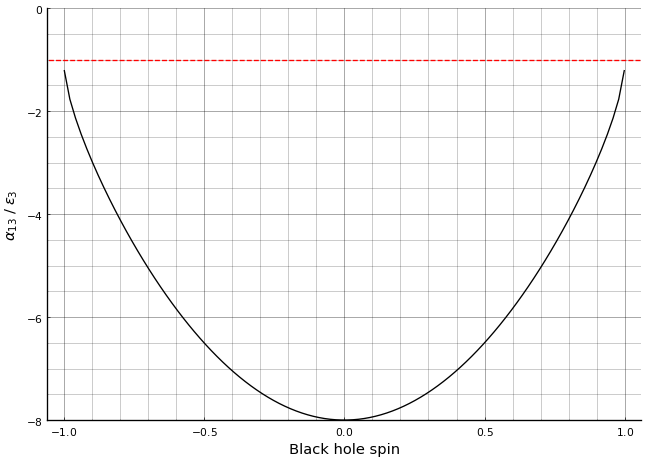
\includegraphics[keepaspectratio]{images/alpha13spin.png}}

\bookmarksetup{startatroot}

\chapter{Developing and Migrating to a Table
Model}\label{developing-and-migrating-to-a-table-model}

\section{Introduction}\label{introduction}

Due to having to render the line profile through Gradus upon every
iteration of the fit, the model took a significant amount of time to fit
to the data. Thus other methods were looked into and it was decided to
develop a table model, allowing for the pre-computation of the line
profiles. The computed profiles could then be interpolated between for a
given set of parameters, significantly speeding up computation. This
would of course decrease the accuracy of the model, however the
increased efficiency would likely be worth that loss.

The structure for XSPEC table models is well documented at
\href{https://heasarc.gsfc.nasa.gov/FTP/caldb/docs/memos/ogip_92_009/ogip_92_009.pdf}{XSPEC
Table Models} ~{[}4{]}, thus the model was constructed using this
specification. \texttt{SpectralFitting.jl} also has compatibility with
this model format, which made integration more viable (see
\href{https://github.com/JuliaAstro/SpectralFitting.jl/blob/main/src/meta-models/table-models.jl}{here}
for more ~{[}5{]}).

\section{Data Generation}\label{data-generation}

The spectra for the model were simply generated by looping through a
defined parameter space, with a given number of values for each of the 5
parameters. The values selected were defined as follows

{\def\LTcaptype{none} % do not increment counter
\begin{longtable}[]{@{}llll@{}}
\toprule\noalign{}
Parameter & Lower Bound & Upper Bound & Number \\
\midrule\noalign{}
\endhead
\bottomrule\noalign{}
\endlastfoot
\(a\) & -0.998 & 0.998 & 7 \\
\(h\) & 1.5 & 30 & 10 \\
\(\theta\) & 5 & 85 & 10 \\
\(\alpha_{13}\) & 0 & 50 & 7 \\
\(\epsilon_3\) & 0 & 30 & 10 \\
\end{longtable}
}

This gave a total of 49,000 combinations to loop through. Seven values
were used for both \(a\) and \(\alpha_{13}\) as they had the smallest,
and most predictable effect on the line profile, respectively. In a
later iteration of this model it would be ideal to have a larger
parameter space to reduce the innacuracies of interpolation, however for
a test case it was necessary to keep compute times down. The line
profiles were stored in columns of a CSV with the header containing the
parameter information.

Certain parameter combinations would fail to compute, and therefore a
log file was kept, noting the combination and when it failed. This
allowed the computations to run over night without risk of an error. The
final compute time for this data generation was 16 hours. 3,500 of the
49,000 did not compute correctly, thus there is 45,500 datapoints in the
grid.

\section{Loading into FITS Format}\label{loading-into-fits-format}

This data was then loaded into a FITS file following the XSPEC model
format using the python wrapper for the \texttt{heasp} C library,
\texttt{heasoftpy} (see the
\href{https://heasarc.gsfc.nasa.gov/docs/software/lheasoft/headas/heasp/node2.html}{documentation}
for more information). The model specification requires that the grid be
rectilinear ~{[}4{]}, thus it was not possible to simply disregard the
failed runs, and the spectra for these combinations was set to be zeroed
out. This was determined to be acceptable as the majority of the failed
runs had large \(\alpha_{13}\) or \(\epsilon_3\), which from earlier
testing was noted to be unlikely during fitting, thus the failed
combinations would be unlikely to be used for interpolation.

\section{The Model}\label{the-model}

To create a model in SpectralFitting using the table, the data was
loaded into a \texttt{TableModelData} struct. This could then be wrapped
using \texttt{TableModelInterpolation} such that it can work with the
\texttt{TableModelInterpolation} function. This functionality made it
trivial to set up the interpolation through the parameter grid by simply
calling

\begin{verbatim}
SpectralFitting.interpolate_table!(table, a, h, θ, α13, ϵ3)
\end{verbatim}

This returned a spectrum with 1000 datapoints, which could then be
interpolated over the domain of the input data. With this architecture
it was simple to fit the data as previous.

\subsection{Performance}\label{performance}

Using the nu80402315002 dataset as before, the new model yielded the
following results.

\begin{figure}[H]

{\centering \pandocbounded{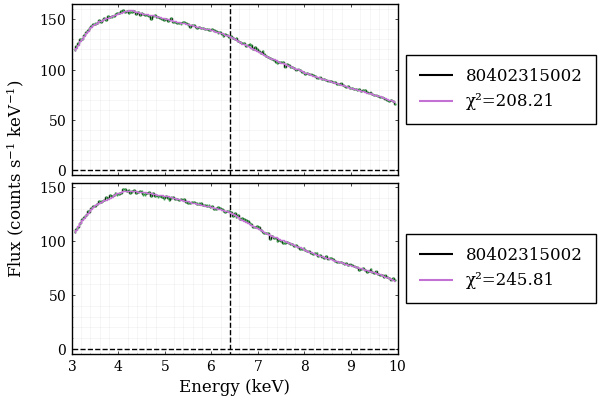
\includegraphics[keepaspectratio]{images/TableKerrnu80402315002.png}}

}

\caption{The table model result for the Kerr metric}

\end{figure}%

\begin{figure}[H]

{\centering \pandocbounded{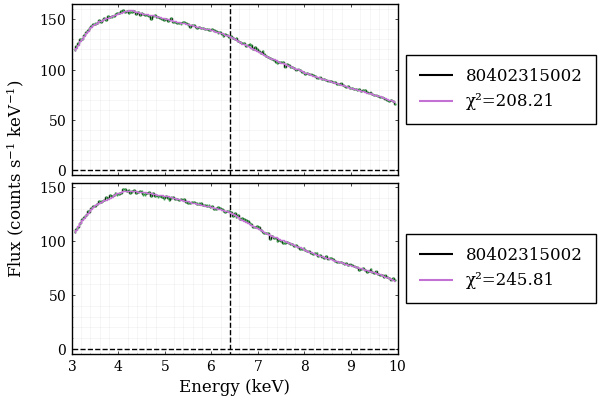
\includegraphics[keepaspectratio]{images/TableJohannsennu80402315002.png}}

}

\caption{The table model result for the Johannsen metric}

\end{figure}%

Comparing to the previous fits, the \(\chi^2\) value for both of these
fits were surprisingly improved. The Kerr fit was completed by freezing
the deformation parameters at 0.

These fits took only 30 seconds to fit and plot both metrics, which was
significantly faster than previous which could take an hour or more for
a single fit.

\section{Next Steps}\label{next-steps}

After review of the log file, it was found that a lot of the cases where
the deformation parameters were zero failed. This is significant as it
implies that many of the Kerr model interpolations are innacurate due to
the ``correction'' method used (setting missing values to zero). Using
code to parse the unique values for each of the 5 parameters, it was
found that every instance of failure had \(h=1.5\). It was thus decided
that upon the next iteration of the model, the lower bound of \(h\)
would be set to 3. This value was determined after some brief testing
with the failed runs, manually setting \(h=3\). \(h=2\) was also
attempted, however this similarly caused errors.

Building on what was discussed in the previous chapter regarding the
lower bounds for the parameters, it was also tested whether a value of
-1 computed correctly for both of the deformation parameters. This was
successful and thus a partial implementation of these bounds can be
completed.

Further testing was also conducted in the parameter space of \(a\) where
it was found that the line profile does not change with the sign of
\(a\). This will allow for much more resolution without increasing the
length of computation.

To use the negative deformation parameters, their allowed values must be
reduced as it is necessary to have confidence in the deformation = 0
(Kerr) cases. They will therefore take the values
\(\alpha_{13}, \epsilon_3 \in [-1, 10], \mathbb{Z}\). The other
variables will take \(h\in[3,15]\), \(a\in[0,0.998]\) and
\(\theta\in [5,85]\). Thus 7 values will be taken for \(a\), 12 for the
deformation parameters, and 9 for \(h,\;\theta\), giving a total size of
81648 for the table.

The final iteration that needs to be made upon the data is to increase
the domain, as the model is currently forced to extrapolate causing
unexpected issues, likely forcing the fitting to take worse values to
avoid these errors.

All of these iterations were implemented and another dataset computed.
At the time of writing these computations are still ongoing and
therefore time was taken to clean up the plotting and do further
reading.

Functionality was then added to plot a contour plot of the fit statistic
(\(\chi^2\)) for a pair of fit parameters. The fits are however not
currently accurate enough to determine the functionality of this plot,
thus this remains to be used.

\section{Current Issues 2026/07/03}\label{current-issues-20260703}

The table model currently does not contain the full set of spectra for
negative values of the deformation parameters. For high spin parameters,
the code will sometimes fail to compute the line profile citing either
one of two errors:

\begin{verbatim}
ErrorException("No boundaries for minimization could be determined. It is likely this configuration does not have an ISCO solution.")
\end{verbatim}

or

\begin{verbatim}
DomainError([VALUE], "sqrt was called with a negative real argument but will only return a complex result if called with a complex argument. Try sqrt(Complex(x)).")
\end{verbatim}

This occurs when attempting to use negative values below \(\sim-0.4\)
for either, or both, of the deformation parameters. This is likely
either a bug, or an artefact of the Johannsen metric. The only currently
known constraints on allowed values of \(\alpha_{13}\) and
\(\epsilon_{3}\) are those stated in Equations
Equation~\ref{eq-Epsilon3Constraint} and
Equation~\ref{eq-Alpha13Constraint}, which all values used satisfy. The
current working theory is thus that this may be a bug with
\texttt{Gradus.jl} however this requires further research.

There also exists the restriction that \(|a|<1\) to avoid a naked
singularity ~{[}6{]}, however this is once again satisfied by the used
values.

The table model is currently capable of extrapolating, which provides
reasonable estimates of the line profile for negative values (see
Figure~\ref{fig-GradusTableCompare}) however it would not be preferable
to rely on extrapolation to constrain the parameters.

\begin{figure}

\centering{

\pandocbounded{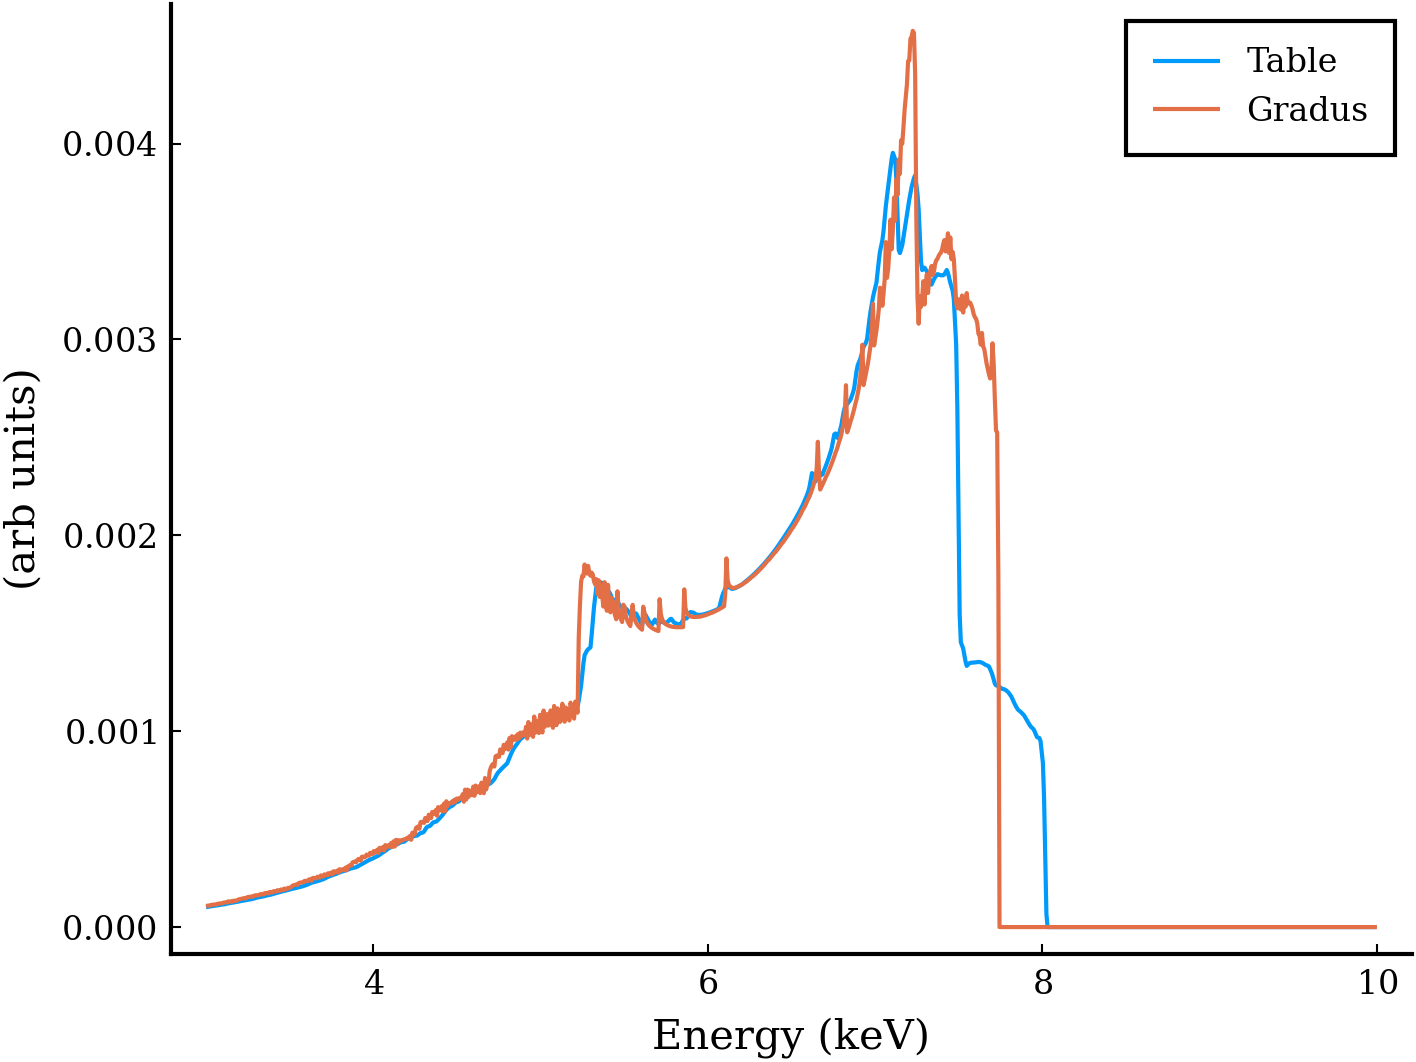
\includegraphics[keepaspectratio]{images/GradusTableCompare.png}}

}

\caption{\label{fig-GradusTableCompare}}

\end{figure}%

\bookmarksetup{startatroot}

\chapter{XRISM Data Reduction}\label{xrism-data-reduction}

These notes are significantly condensed and adapted from the XRISM Quick
Start Guide ~{[}7{]}. All key steps for the reduction are on this page,
however some details and steps to deal with specific issues have been
omitted for brevity. I have noted where applicable where to go for more
information.

\begin{tcolorbox}[enhanced jigsaw, arc=.35mm, bottomrule=.15mm, bottomtitle=1mm, breakable, colback=white, colbacktitle=quarto-callout-important-color!10!white, colframe=quarto-callout-important-color-frame, coltitle=black, left=2mm, leftrule=.75mm, opacityback=0, opacitybacktitle=0.6, rightrule=.15mm, title=\textcolor{quarto-callout-important-color}{\faExclamation}\hspace{0.5em}{Notes}, titlerule=0mm, toprule=.15mm, toptitle=1mm]

\begin{itemize}
\tightlist
\item
  All commands below assume that HEASOFT and CalDB are installed and
  instantiated, and that the CalDB installation has the
  \href{https://heasarc.gsfc.nasa.gov/docs/xrism/calib/index.html}{necessary
  files} for XRISM data.
\item
  Data will have observation ID as top directory, e.g.~000125000/
\item
  Pipeline scripts must be run in a directory that contains this
  directory
\item
  The
  \href{https://heasarc.gsfc.nasa.gov/docs/xrism/analysis/abc_guide/xrism_abc.html}{XRISM
  Data Analysis Guide} contains more information relevant to this
  process.
\end{itemize}

\end{tcolorbox}

\section{Pipeline Scripts}\label{pipeline-scripts}

For all following commands replace \texttt{000125000} with the
observation id for your data. The commands in this section have been
streamlined with InitialPipeline.sh for \texttt{bash} systems.

\subsection{Reprocessing:}\label{reprocessing}

In the directory above data directory run the following for the resolve
data

\begin{Shaded}
\begin{Highlighting}[]
\CommentTok{\# Run the pipeline}
\ExtensionTok{xapipeline}\NormalTok{ indir=000125000 outdir=000125000\_rsl\_reproc steminputs=xa000125000 stemoutputs=DEFAULT entry\_stage=1 exit\_stage=3 instrument=resolve verify\_input=no create\_ehkmkf=no calc\_pointing=yes calc\_optaxis=yes calc\_gtilost=no calc\_adrgti=no calc\_mxsgti=no rsl\_gainfile=CALDB calmethod=FE55 linetocorrect=MnKa seed=650504 numevent=1000 minevent=200 extraspread=40 spangti=no}
\end{Highlighting}
\end{Shaded}

Then for the Xtend data

\begin{Shaded}
\begin{Highlighting}[]
\CommentTok{\# Run the pipeline}
\ExtensionTok{xapipeline}\NormalTok{ indir=000125000 outdir=000125000\_xtd\_reproc steminputs=xa000125000 stemoutputs=DEFAULT entry\_stage=1 exit\_stage=3 instrument=xtend verify\_input=no create\_ehkmkf=no calc\_pointing=yes calc\_optaxis=yes seed=650504}
\end{Highlighting}
\end{Shaded}

The \texttt{.hk} files can be removed as they are duplicates of the
corresponding files in the original data. The remaining files can be
gzipped for space efficiency. \texttt{InitialPipeline.sh} does this
automatically.

\subsection{Analysis Setup}\label{analysis-setup}

Then make a directory for the analysis and copy the following files

\begin{Shaded}
\begin{Highlighting}[]
\FunctionTok{mkdir}\NormalTok{ analysis}

\FunctionTok{cp}\NormalTok{ 000125000\_xtd\_reproc/}\PreprocessorTok{*}\NormalTok{\_cl.evt.gz analysis/}
\FunctionTok{cp}\NormalTok{ 000125000\_rsl\_reproc/}\PreprocessorTok{*}\NormalTok{\_cl.evt.gz analysis/}
\FunctionTok{cp}\NormalTok{ 000125000\_rsl\_reproc/xa000125000.ehk.gz 000125000\_rsl\_reproc/xa000125000rsl\_px1000\_exp.gti.gz 000125000\_xtd\_reproc/xa000125000xtd\_p031100010.bimg.gz analysis/}
\end{Highlighting}
\end{Shaded}

You will also need the \texttt{RA\_NOM}, \texttt{PA\_NOM}, and
\texttt{DEC\_NOM} values from the Resolve header which can be obtained
with

\begin{Shaded}
\begin{Highlighting}[]
\CommentTok{\# Getting Resolve RA, DEC, PA and storing in a file}
\ExtensionTok{ftlist}\NormalTok{ xa}\StringTok{"}\VariableTok{$OBSID}\StringTok{"}\NormalTok{rsl\_p0px1000\_cl.evt.gz K }\KeywordTok{|} \FunctionTok{grep} \AttributeTok{{-}m}\NormalTok{ 3 }\AttributeTok{{-}e}\NormalTok{ DEC\_NOM }\AttributeTok{{-}e}\NormalTok{ RA\_NOM }\AttributeTok{{-}e}\NormalTok{ PA\_NOM }\OperatorTok{\textgreater{}}\NormalTok{ rsl\_coordinates.txt}
\end{Highlighting}
\end{Shaded}

This will write the three values to a text file

\subsection{PSP Limit Checks}\label{psp-limit-checks}

Run PSP limit check to see if the unscreened count rate for Resolve
exceeds the psp limit in the \texttt{000125000\_rsl\_reproc/} directory.

\begin{Shaded}
\begin{Highlighting}[]
\ExtensionTok{rslbratios}\NormalTok{ infile=xa000125000rsl\_p0px1000\_uf.evt.gz filetype=uf outroot=rsl000125000\_ufbr}
\end{Highlighting}
\end{Shaded}

This gives a info on if quadrants exceed 50 cts s\^{}-1, which makes the
data unusable. A log file is produced which lists the pixels that exceed
the limit, these only apply to Resolve data, and these pixels will be
unusable.

Next run rslbratios on the cleaned resolve data in the
\texttt{analysis/} directory:

\begin{Shaded}
\begin{Highlighting}[]
\ExtensionTok{rslbratios}\NormalTok{ infile=xa000125000rsl\_p0px1000\_cl.evt.gz filetype=cl outroot=rsl000125000\_clbr lcbin=128.0}
\end{Highlighting}
\end{Shaded}

This gives the same info but for the cleaned data and outputs the
following files which will be used later

\begin{itemize}
\tightlist
\item
  \texttt{rsl000125000\_clbr\_2keVto12keV\_hist.fits}: Observed
  vs.~predicted branching ratios in the energy range specified by the
  ``eband'' parameter
\item
  \texttt{rsl000125000\_clbr\_full\_lc.fits}: Full array light curves by
  grade
\item
  \texttt{rsl000125000\_clbr\_pix\_lc.fits}: Per-pixel light curves by
  grade
\item
  \texttt{rsl000125000\_clbr\_gradeFrac\_lc.fits}: Grade fractions
  versus time
\item
  \texttt{rsl000125000\_clbr\_2keVto12keV\_pixMap.img}: 20 images of
  counts by grade, and grade fractions for two energy bands
\end{itemize}

\section{Removing Anomalous Pixels from Xtend
Data}\label{removing-anomalous-pixels-from-xtend-data}

\begin{tcolorbox}[enhanced jigsaw, arc=.35mm, bottomrule=.15mm, bottomtitle=1mm, breakable, colback=white, colbacktitle=quarto-callout-important-color!10!white, colframe=quarto-callout-important-color-frame, coltitle=black, left=2mm, leftrule=.75mm, opacityback=0, opacitybacktitle=0.6, rightrule=.15mm, title=\textcolor{quarto-callout-important-color}{\faExclamation}\hspace{0.5em}{Important}, titlerule=0mm, toprule=.15mm, toptitle=1mm]

All following commands are run from the \texttt{analysis/} directory

\end{tcolorbox}

\begin{tcolorbox}[enhanced jigsaw, arc=.35mm, bottomrule=.15mm, bottomtitle=1mm, breakable, colback=white, colbacktitle=quarto-callout-note-color!10!white, colframe=quarto-callout-note-color-frame, coltitle=black, left=2mm, leftrule=.75mm, opacityback=0, opacitybacktitle=0.6, rightrule=.15mm, title=\textcolor{quarto-callout-note-color}{\faInfo}\hspace{0.5em}{Note}, titlerule=0mm, toprule=.15mm, toptitle=1mm]

This section makes heavy use of \texttt{xtdpixclip}, and the usage is
not documented in the XRISM QSG, see the \texttt{xtdpixclip}
documentation ~{[}8{]} for more information.

\end{tcolorbox}

First generate region files using ds9, viewing the image in DET
coordinates with the command.

\begin{Shaded}
\begin{Highlighting}[]
\ExtensionTok{ds9} \StringTok{"xa000125000xtd\_p031100010\_cl.evt.gz[bin=detx,dety]"}
\end{Highlighting}
\end{Shaded}

\begin{figure}[H]

{\centering \pandocbounded{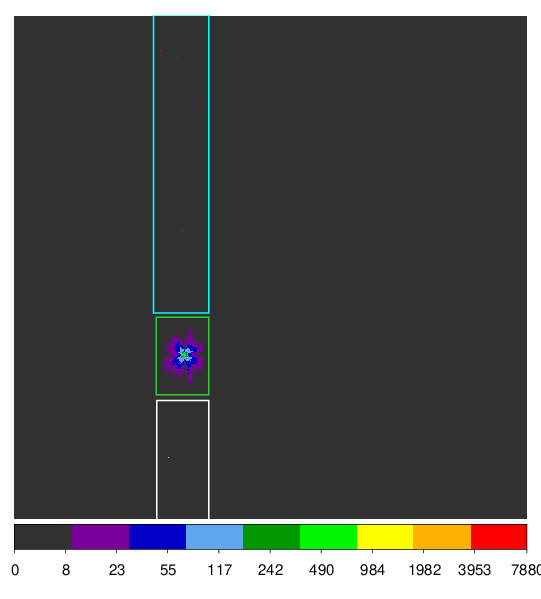
\includegraphics[keepaspectratio]{images/Regions.png}}

}

\caption{The regions used.}

\end{figure}%

Three regions were selected and labelled as follows:

\begin{itemize}
\tightlist
\item
  White: \texttt{1\_bottom.reg}
\item
  Green: \texttt{1\_src.reg}
\item
  Cyan: \texttt{1\_top.reg}
\end{itemize}

Next run xtdpixclip in histogram mode to generate histograms for the
regions, including all of the region files just generated.

\begin{Shaded}
\begin{Highlighting}[]
\ExtensionTok{punlearn}\NormalTok{ xtdpixclip}
\ExtensionTok{xtdpixclip}\NormalTok{ evtinfile=}\StringTok{"xa000125000xtd\_p031100010\_cl.evt.gz"}\NormalTok{ outroot=}\StringTok{"xa000125000xtd\_p031100010\_cl"}\NormalTok{ pmode=histo nhistbins={-}1 incregionfiles=}\StringTok{"1\_top.reg,1\_bottom.reg,1\_src.reg"}\NormalTok{ emax=24.575 chatter=2 clobber=yes}
\end{Highlighting}
\end{Shaded}

These histograms can be used to determine the thresholds to use as
cutoffs for anomolous pixels. The output histograms are shown below

\begin{figure}

\begin{minipage}[t]{0.50\linewidth}

\begin{figure}[H]

{\centering \pandocbounded{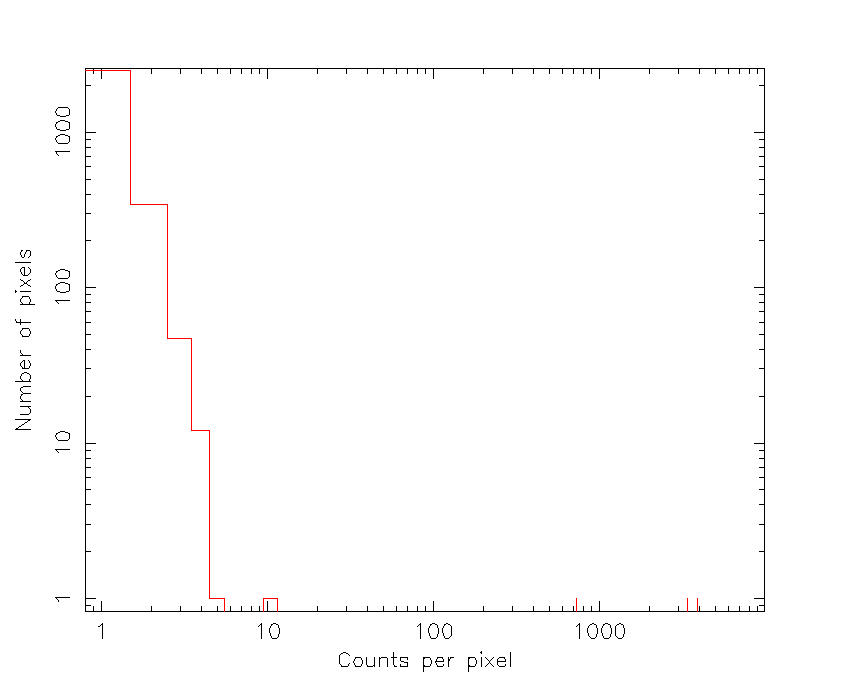
\includegraphics[keepaspectratio]{images/BottomRegion.png}}

}

\subcaption{The bottom region histogram}

\end{figure}%

\end{minipage}%
%
\begin{minipage}[t]{0.50\linewidth}

\begin{figure}[H]

{\centering \pandocbounded{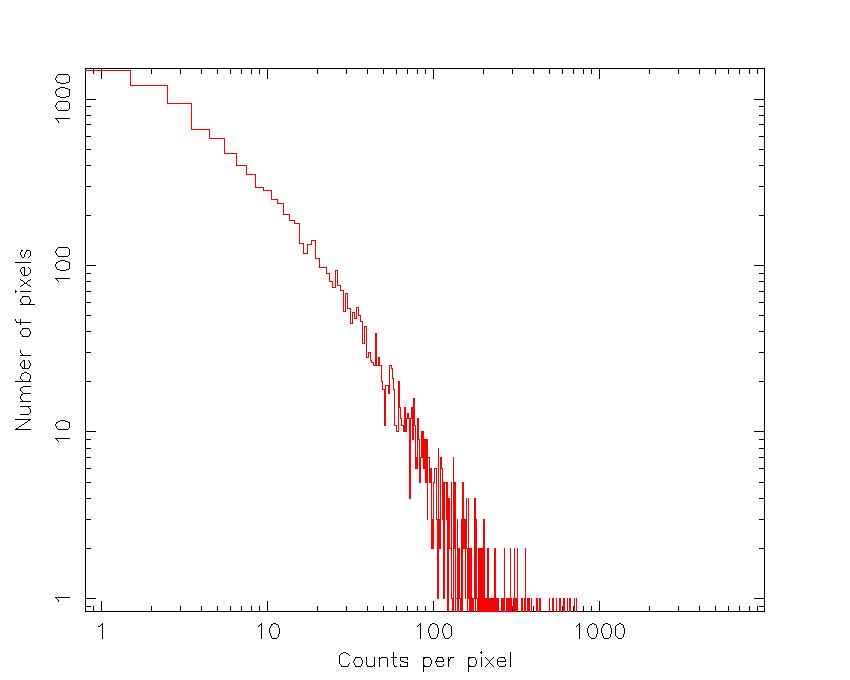
\includegraphics[keepaspectratio]{images/SourceRegion.png}}

}

\subcaption{The source region histogram}

\end{figure}%

\end{minipage}%
\newline
\begin{minipage}[t]{0.50\linewidth}

\begin{figure}[H]

{\centering \pandocbounded{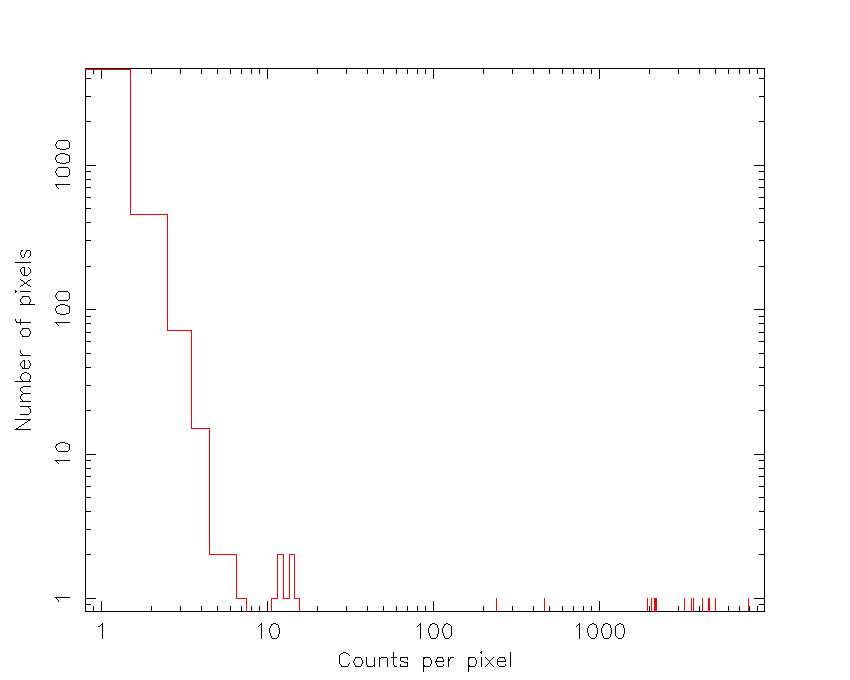
\includegraphics[keepaspectratio]{images/TopRegion.png}}

}

\subcaption{The top region histogram}

\end{figure}%

\end{minipage}%

\end{figure}%

For the two non-source regions a threshold of 8 was selected, and for
the source region 1000 was selected. With the regions selected run
xtdpixclip again but in apply mode, entering the thresholds selected

\begin{Shaded}
\begin{Highlighting}[]
\ExtensionTok{punlearn}\NormalTok{ xtdpixclip}
\ExtensionTok{xtdpixclip}\NormalTok{ evtinfile=}\StringTok{"xa000125000xtd\_p031100010\_cl.evt.gz"}\NormalTok{ outroot=}\StringTok{"xa000125000xtd\_p031100010\_cl"}\NormalTok{ pmode=apply thresholds=}\StringTok{"8,8,1000"}\NormalTok{ incregionfiles=}\StringTok{"1\_top.reg,1\_bottom.reg,1\_src.reg"}\NormalTok{ emax=24.575 chatter=2 clobber=yes}
\end{Highlighting}
\end{Shaded}

\begin{figure}

\begin{minipage}[t]{0.50\linewidth}

\begin{figure}[H]

{\centering \pandocbounded{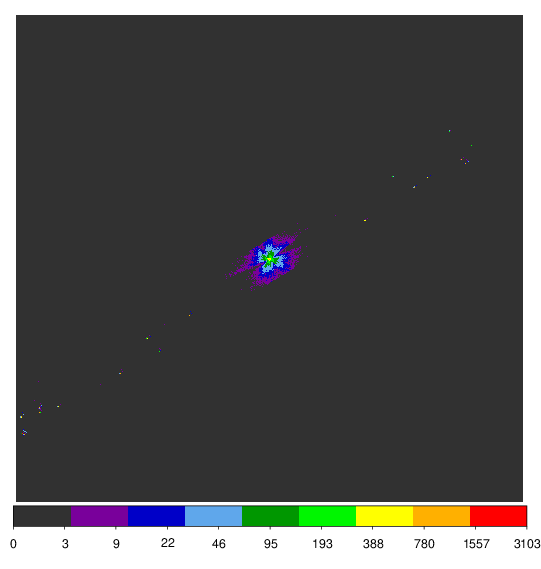
\includegraphics[keepaspectratio]{images/Raw.png}}

}

\subcaption{The Raw image}

\end{figure}%

\end{minipage}%
%
\begin{minipage}[t]{0.50\linewidth}

\begin{figure}[H]

{\centering \pandocbounded{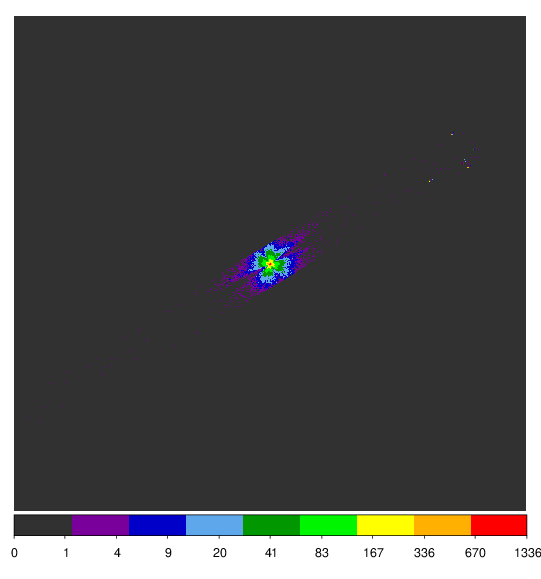
\includegraphics[keepaspectratio]{images/Clean.png}}

}

\subcaption{The cleaned image}

\end{figure}%

\end{minipage}%
\newline
\begin{minipage}[t]{0.50\linewidth}

\begin{figure}[H]

{\centering \pandocbounded{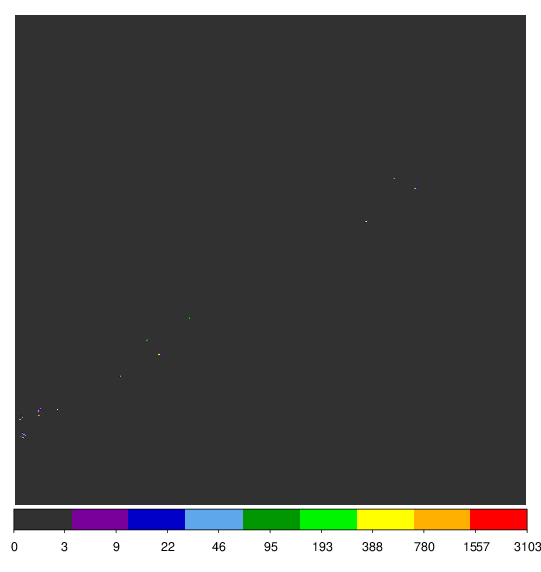
\includegraphics[keepaspectratio]{images/BadPX.png}}

}

\subcaption{The filtered out pixels}

\end{figure}%

\end{minipage}%

\end{figure}%

\section{Proximity and Rise time
screening}\label{proximity-and-rise-time-screening}

\begin{itemize}
\tightlist
\item
  Proximity screening: Removing frame events based on the unlikelihood
  of events happening too close together in a given time interval. This
  must be balanced against the loss of counts.
\end{itemize}

The effect of both can be previewed through the files:

\begin{verbatim}
rsl000125000_clbr_prox_Hp_spectra.fits
rsl000125000_clbr_rise_Hp_spectra.fits
\end{verbatim}

These can be examined by plotting the difference after proximity and
rise-screening to observe the losses. This can be done with fplot:

\begin{Shaded}
\begin{Highlighting}[]
\CommentTok{\# For Proximity Screening}
\ExtensionTok{fplot}\NormalTok{ rsl000125000\_clbr\_prox\_Hp\_spectra.fits}\PreprocessorTok{[}\SpecialStringTok{DIFFERENCE}\PreprocessorTok{]}\NormalTok{ PI DIFF }\AttributeTok{{-}}\NormalTok{ /PS Q}

\CommentTok{\# For Rise{-}Time Screening}
\ExtensionTok{fplot}\NormalTok{ rsl000125000\_clbr\_rise\_Hp\_spectra.fits}\PreprocessorTok{[}\SpecialStringTok{DIFFERENCE}\PreprocessorTok{]}\NormalTok{ PI DIFF }\AttributeTok{{-}}\NormalTok{ /PS Q}
\end{Highlighting}
\end{Shaded}

\begin{figure}

\begin{minipage}[t]{0.50\linewidth}

\begin{figure}[H]

{\centering \pandocbounded{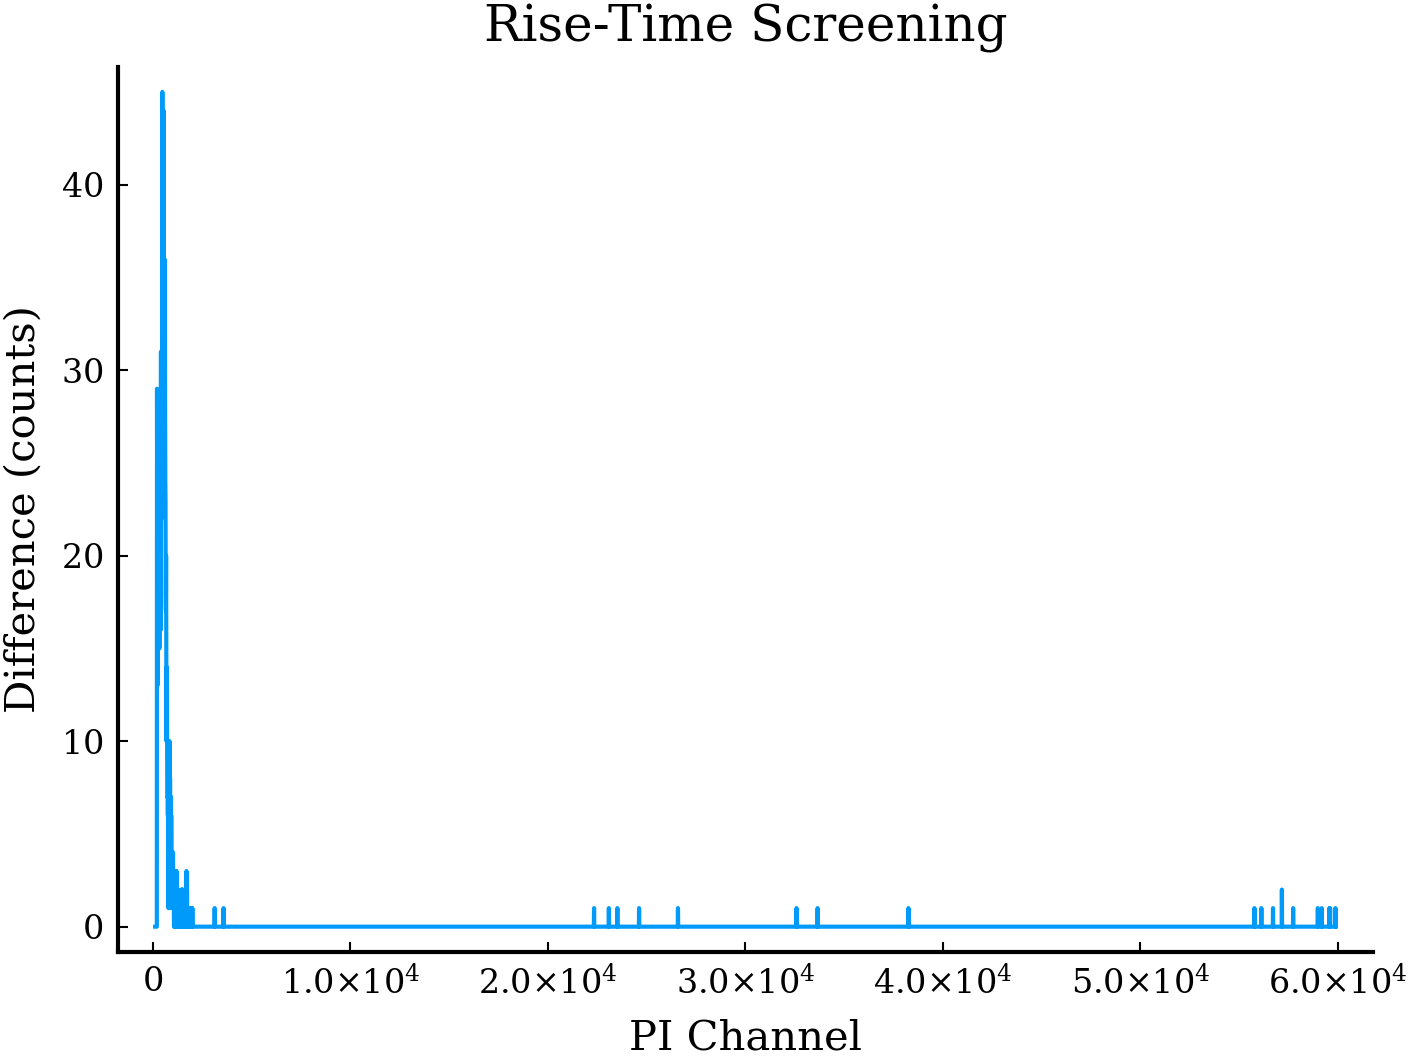
\includegraphics[keepaspectratio]{images/RiseTime.png}}

}

\subcaption{The Rise-time filtering difference}

\end{figure}%

\end{minipage}%
%
\begin{minipage}[t]{0.50\linewidth}

\begin{figure}[H]

{\centering \pandocbounded{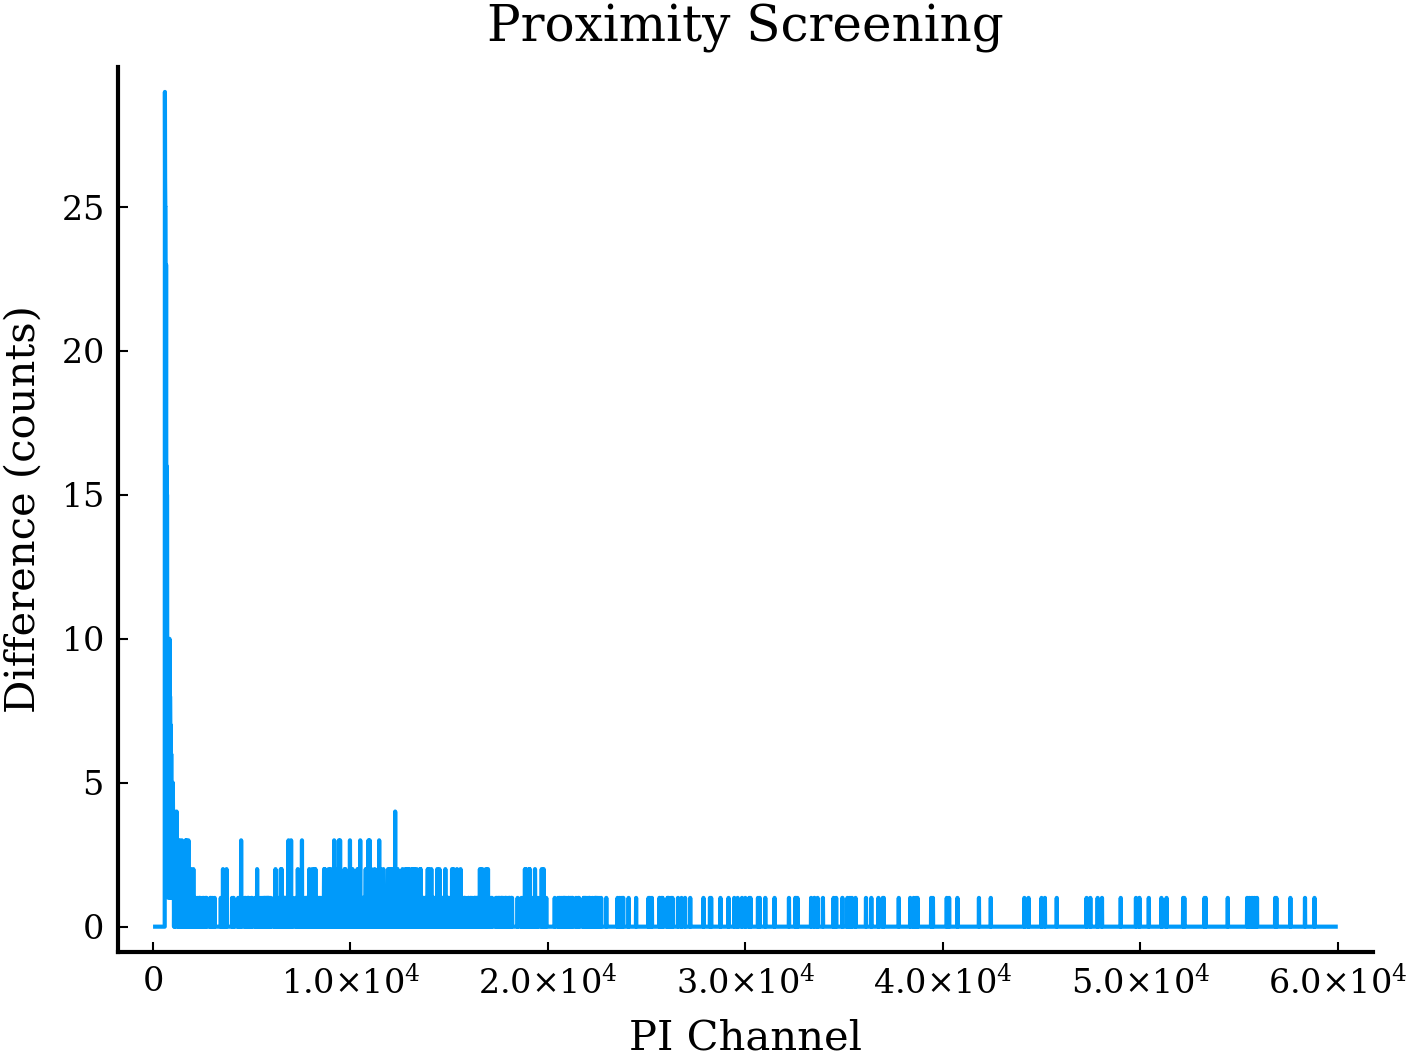
\includegraphics[keepaspectratio]{images/Proximity.png}}

}

\subcaption{The Proximity filtering difference}

\end{figure}%

\end{minipage}%

\end{figure}%

The losses for each were determined to be acceptable for this dataset,
thus the both filters were applied with the command:

\begin{Shaded}
\begin{Highlighting}[]
\ExtensionTok{ftcopy}\NormalTok{ infile=}\StringTok{"xa000125000rsl\_p0px1000\_cl.evt[EVENTS][(PI\textgreater{}=600) \&\& (((((RISE\_TIME+0.00075*DERIV\_MAX)\textgreater{}46)\&\&((RISE\_TIME+0.00075*DERIV\_MAX)\textless{}58))\&\&ITYPE\textless{}4)||(ITYPE==4))\&\&STATUS[4]==b0]"}\NormalTok{ outfile=xa000125000rsl\_p0px1000\_cl2.evt copyall=yes clobber=yes history=yes}
\end{Highlighting}
\end{Shaded}

To skip proximity filtering you can omit \texttt{\&\&STATUS{[}4{]}==b0}.

\begin{tcolorbox}[enhanced jigsaw, arc=.35mm, bottomrule=.15mm, bottomtitle=1mm, breakable, colback=white, colbacktitle=quarto-callout-note-color!10!white, colframe=quarto-callout-note-color-frame, coltitle=black, left=2mm, leftrule=.75mm, opacityback=0, opacitybacktitle=0.6, rightrule=.15mm, title=\textcolor{quarto-callout-note-color}{\faInfo}\hspace{0.5em}{Note}, titlerule=0mm, toprule=.15mm, toptitle=1mm]

The QSG includes a section here on the \texttt{xaspecratios} tool which
is not available until HEASoft 6.37 and is therefore omitted from these
notes.

\end{tcolorbox}

\section{Extract Broadband Images and Establish Source Center
Coordinates}\label{extract-broadband-images-and-establish-source-center-coordinates}

\begin{itemize}
\tightlist
\item
  Check the value of the EXPOSURE keyword in the cleaned event files, if
  the exposure time is unexpectedly low then consult section 9 of the
  QSG ~{[}7{]}.
\item
  You should now have the following files

  \begin{itemize}
  \tightlist
  \item
    \texttt{xa000125000rsl\_p0px1000\_cl2.evt} (Resolve) and
  \item
    \texttt{xa000125000xtd\_p031100010\_cl.evt} or
    \texttt{xa000125000xtd\_p031100010\_xpc\_clnevt.fits} (Xtend)
  \end{itemize}
\end{itemize}

Start XSELECT and make a 2-10 keV resolve image in DET coordinates as:

\begin{Shaded}
\begin{Highlighting}[]
\BuiltInTok{read} \VariableTok{eve} \VariableTok{xa000125000rsl\_p0px1000\_cl2}\NormalTok{.evt .}
\BuiltInTok{set}\NormalTok{ image DET}
\ExtensionTok{filter}\NormalTok{ pha\_cutoff 4000 20000}
\ExtensionTok{extr}\NormalTok{ image}
\ExtensionTok{save}\NormalTok{ image xa000125000rsl\_p0px1000\_detimg.fits}
\end{Highlighting}
\end{Shaded}

Observing this image in \texttt{ds9} or otherwise, \emph{the centre of
the source in the Resolve data should be noted down}. This should be
close to (3.5, 3.5), however we only need to estimate this approximately
as it is used as a sanity check against the RA and DEC coordinates. For
most standard observations we can simply assume this centre coordinate.

Next copy over a resolve region file from the \texttt{\$HEADAS}
directory.

\begin{Shaded}
\begin{Highlighting}[]
\FunctionTok{cp} \VariableTok{$HEADAS}\NormalTok{/refdata/region\_RSL\_det.reg .}
\end{Highlighting}
\end{Shaded}

and make another region file \texttt{exclude\_calsource.reg} containing

\begin{verbatim}
physical
-circle(920.0,1530.0,92.0)
-circle(919.0,271.0,91.0)
\end{verbatim}

using

\begin{Shaded}
\begin{Highlighting}[]
\BuiltInTok{echo} \StringTok{"physical"} \OperatorTok{\textgreater{}}\NormalTok{ exclude\_calsources.reg}
\BuiltInTok{echo} \StringTok{"{-}circle(920.0,1530.0,92.0)"} \OperatorTok{\textgreater{}\textgreater{}}\NormalTok{ exclude\_calsources.reg}
\BuiltInTok{echo} \StringTok{"{-}circle(919.0,271.0,91.0)"} \OperatorTok{\textgreater{}\textgreater{}}\NormalTok{ exclude\_calsources.reg}
\end{Highlighting}
\end{Shaded}

Next make a 0.5-10 keV Xtend image in DET coordinates

\begin{Shaded}
\begin{Highlighting}[]
\FunctionTok{clear}\NormalTok{ all}
\BuiltInTok{read} \VariableTok{eve} \VariableTok{xa000125000xtd\_p031100010\_cl\_xpc\_clnevt}\NormalTok{.fits .}
\BuiltInTok{set}\NormalTok{ image DET}
\ExtensionTok{filter}\NormalTok{ region exclude\_calsources.reg}
\ExtensionTok{filter}\NormalTok{ pha\_cutoff 83 1667}
\ExtensionTok{extr}\NormalTok{ image}
\ExtensionTok{save}\NormalTok{ image xa000125000xtd\_p031100010\_detimg.fits}
\end{Highlighting}
\end{Shaded}

Now we can estimate the centroid of the source in DET coordinates in the
Xtend data using \texttt{ds9}. \emph{Note this coordinate down as it
will also be useful later}.

Next make region files for the source and background lightcurves and
spectra. It is reccommended to use a rectangle of length 5 arcmin and
width as wide as possible for 1/8 Window mode images. The region should
not extend beyond the chip boundary as this will result in an incorrect
ARF. For full window mode it is reccommended to use a circle of radius
2.5 arcmin. The regions selected for the data used here are shown below

\begin{center}
\pandocbounded{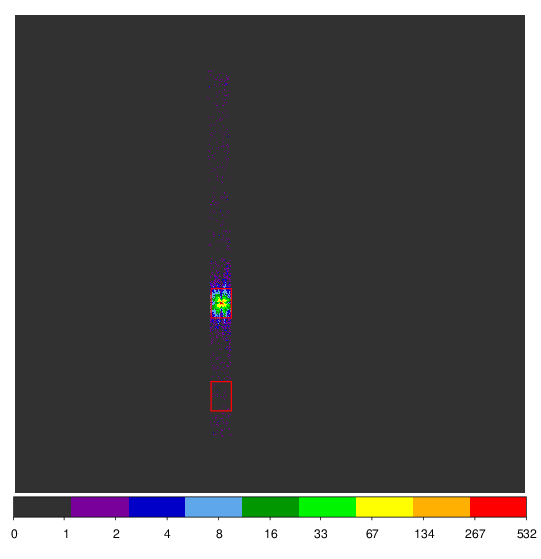
\includegraphics[keepaspectratio]{images/SourceBgdRegions.png}}
\end{center}

and were saved as

\begin{verbatim}
region_000125000xtd_src.reg
region_000125000xtd_bgd.reg
\end{verbatim}

\section{Extract Lightcurves and
Spectra}\label{extract-lightcurves-and-spectra}

In the \texttt{analysis/} directory start a new XSELECT session and read
in the cleaned resolve event file:

\begin{Shaded}
\begin{Highlighting}[]
\BuiltInTok{read} \VariableTok{eve} \VariableTok{xa000125000rsl\_p0px1000\_cl2}\NormalTok{.evt .}

\CommentTok{\# Extract a resolve full{-}array lightcurve in the 2{-}10 keV band (time bin in seconds)}
\BuiltInTok{set}\NormalTok{ image det}
\ExtensionTok{filter}\NormalTok{ pha\_cutoff 4000 20000}
\BuiltInTok{set}\NormalTok{ binsize 128.0}
\ExtensionTok{extr}\NormalTok{ curve exposure=0.8}
\ExtensionTok{save}\NormalTok{ curve xa000125000rsl\_allpix\_b128\_lc.fits}

\CommentTok{\# If a time bin has less than a fraction "exposure" then you will get a warning about too many bins being cut, reduce the value of exposure to mitigate this}

\CommentTok{\# Extract a Resolve spectrum from the full array, for hi{-}res primary events only}
\CommentTok{\# The first command can be modified to exclude pixels or a group of pixels}
\ExtensionTok{filter}\NormalTok{ column }\StringTok{"pixel=0:11,13:35"}
\ExtensionTok{filter}\NormalTok{ GRADE }\StringTok{"0:0"}
\ExtensionTok{extr}\NormalTok{ spectrum}
\ExtensionTok{save}\NormalTok{ spectrum xa000125000rsl\_allpix\_Hp\_src.pi}

\CommentTok{\# Read in the cleaned Xtend event file and extract 0.5{-}10 keV lightcurves and spectra from the background and source regions}
\FunctionTok{clear}\NormalTok{ all}
\BuiltInTok{read} \VariableTok{eve} \VariableTok{xa000125000xtd\_p031100010\_cl\_xpc\_clnevt}\NormalTok{.fits .}
\BuiltInTok{set}\NormalTok{ image det}
\ExtensionTok{filter}\NormalTok{ region region\_000125000xtd\_bgd.reg}
\ExtensionTok{filter}\NormalTok{ pha\_cutoff 83 1667}
\BuiltInTok{set}\NormalTok{ binsize 128.0}
\ExtensionTok{extr}\NormalTok{ curve exposure=0.4}
\ExtensionTok{save}\NormalTok{ curve xa000125000xtd\_0p5to10keV\_b128\_bgd\_lc.fits}
\FunctionTok{clear}\NormalTok{ pha\_cutoff}
\ExtensionTok{extr}\NormalTok{ spectrum}
\ExtensionTok{save}\NormalTok{ spectrum xa000125000xtd\_bgd.pi}
\FunctionTok{clear}\NormalTok{ region}
\ExtensionTok{filter}\NormalTok{ region region\_000125000xtd\_src.reg}
\ExtensionTok{filter}\NormalTok{ pha\_cutoff 83 1667}
\ExtensionTok{extr}\NormalTok{ curve exposure=0.4}
\ExtensionTok{save}\NormalTok{ curve xa000125000xtd\_0p5to10keV\_b128\_src\_lc.fits}
\FunctionTok{clear}\NormalTok{ pha\_cutoff}
\ExtensionTok{extr}\NormalTok{ spectrum}
\ExtensionTok{save}\NormalTok{ spectrum xa000125000xtd\_src.pi}
\BuiltInTok{exit}
\end{Highlighting}
\end{Shaded}

\section{Check Attitude Stability}\label{check-attitude-stability}

\begin{Shaded}
\begin{Highlighting}[]
\ExtensionTok{ftselect}\NormalTok{ infile=xa000125000.ehk outfile=xa000125000\_gtifiltered.ehk }
\CommentTok{\# Using the expression:}
\ExtensionTok{gtifilter}\ErrorTok{(}\StringTok{"xa000125000rsl\_p0px1000\_cl2.evt[GTI]"}\KeywordTok{)}

\ExtensionTok{fplot}\NormalTok{ xa000125000\_gtifiltered.ehk TIME ANG\_DIST }\AttributeTok{{-}}\NormalTok{ /PS Q outfile=attitudestability.ps}
\end{Highlighting}
\end{Shaded}

Examine the attitude stability during the observation (e.g.~by plotting
ANG\_DIST versus TIME for the ``xa000125000\_gtifiltered.ehk'' file)

If you need to extract products with stricter attitude stability, make
an appropriate GTI file. You can also make ARFs that are based on more
than one attitude bin. Read the help for xaexpmap and xaarfgen for
guidance on how to do that.

\section{Make Exposure Map/Attitude Histogram
Files}\label{make-exposure-mapattitude-histogram-files}

The following examples make histograms with one attitude bin, which
should be good enough for the majority of cases.

\begin{tcolorbox}[enhanced jigsaw, arc=.35mm, bottomrule=.15mm, bottomtitle=1mm, breakable, colback=white, colbacktitle=quarto-callout-warning-color!10!white, colframe=quarto-callout-warning-color-frame, coltitle=black, left=2mm, leftrule=.75mm, opacityback=0, opacitybacktitle=0.6, rightrule=.15mm, title=\textcolor{quarto-callout-warning-color}{\faExclamationTriangle}\hspace{0.5em}{Mitigation of a bug in CalDB 12 and HEASoft 6.36}, titlerule=0mm, toprule=.15mm, toptitle=1mm]

If you are using CalDB 12 and HEASoft 6.36, there is a bug related to
new optical axes offsets that affect the ARF calculation, which will be
fixed in subsequent CalDB and software releases. Until then, a
mitigation strategy is applied, as shown in commands below, that reverts
creation of the ARF to be the same as if the previous CalDB and software
versions were used.

\end{tcolorbox}

For Resolve:

\begin{Shaded}
\begin{Highlighting}[]
\ExtensionTok{punlearn}\NormalTok{ xaexpmap}

\ExtensionTok{xaexpmap}\NormalTok{ ehkfile=xa000125000.ehk.gz gtifile=xa000125000rsl\_p0px1000\_cl2.evt instrume=RESOLVE badimgfile=NONE pixgtifile=xa000125000rsl\_px1000\_exp.gti.gz outfile=xa000125000rsl\_p0px1000.expo outmaptype=EXPOSURE delta=20.0 numphi=1 stopsys=SKY instmap=CALDB qefile=CALDB contamifile=CALDB vigfile=CALDB obffile=CALDB fwfile=CALDB gvfile=CALDB maskcalsrc=yes fwtype=FILE specmode=MONO specfile=spec.fits specform=FITS evperchan=DEFAULT abund=1 cols=0 covfac=1 clobber=yes chatter=1 logfile=make\_expo\_xa000125000rsl\_p0px1000.log}
\end{Highlighting}
\end{Shaded}

For CalDB 12 and HEASoft 6.36 mitigation:

\begin{Shaded}
\begin{Highlighting}[]
\ExtensionTok{fparkey}\NormalTok{ fitsfile=xa000125000rsl\_p0px1000.expo keyword=OPTAOFFX value=0.0 comm=}\StringTok{"optical axis X offset reset to 0"}
\ExtensionTok{fparkey}\NormalTok{ fitsfile=xa000125000rsl\_p0px1000.expo keyword=OPTAOFFY value=0.0 comm=}\StringTok{"optical axis Y offset reset to 0"}
\end{Highlighting}
\end{Shaded}

For Xtend:

\begin{Shaded}
\begin{Highlighting}[]
\ExtensionTok{xaexpmap}\NormalTok{ ehkfile=xa000125000.ehk.gz gtifile=xa000125000xtd\_p031100010\_cl\_xpc\_clnevt.fits instrume=XTEND badimgfile=xa000125000xtd\_p031100010.bimg.gz pixgtifile=xa000125000xtd\_p031100010\_cl\_xpc\_rmvpix.fpix outfile=xa000125000xtd\_a031100010.expo outmaptype=EXPOSURE delta=20.0 numphi=1 stopsys=SKY instmap=CALDB qefile=CALDB contamifile=CALDB vigfile=CALDB obffile=CALDB fwfile=CALDB gvfile=CALDB maskcalsrc=yes fwtype=FILE specmode=MONO specfile=spec.fits specform=FITS evperchan=DEFAULT abund=1 cols=0 covfac=1 clobber=yes chatter=1 logfile=make\_expo\_xa000125000xtd\_p031100010.log}
\end{Highlighting}
\end{Shaded}

For CalDB 12 and HEASoft 6.36:

\begin{Shaded}
\begin{Highlighting}[]
\ExtensionTok{fparkey}\NormalTok{ fitsfile=xa000125000xtd\_a031100010.expo keyword=OPTAOFFX value=0.0 comm=}\StringTok{"optical axis X offset reset to 0"}
\ExtensionTok{fparkey}\NormalTok{ fitsfile=xa000125000xtd\_a031100010.expo keyword=OPTAOFFY value=0.0 comm=}\StringTok{"optical axis Y offset reset to 0"}
\end{Highlighting}
\end{Shaded}

\section{Making Spectral Response
Files}\label{making-spectral-response-files}

Two methods are listed in the QSG, for these notes I used the first.

\subsection{Checking Coordinates}\label{checking-coordinates}

We first check the coordinates through \texttt{coordpnt} for each
instrument. Replace \texttt{"RDETX0,\ RDETY0"}, and
\texttt{"XDETX0,\ XDETY0"} with the coordinates relevant to the Resolve
and Xtend data noted down earlier. \texttt{RA\_NOM}, \texttt{DEC\_NOM},
and \texttt{PA\_NOM} can be taken from the \texttt{rsl\_coordinates.txt}
file generated earlier.

\begin{Shaded}
\begin{Highlighting}[]
\ExtensionTok{punlearn}\NormalTok{ coordpnt}
\ExtensionTok{coordpnt}\NormalTok{ input=}\StringTok{"RDETX0,RDETY0"}\NormalTok{ outfile=NONE telescop=XRISM instrume=RESOLVE teldeffile=CALDB startsys=DET stopsys=RADEC ra=RA\_NOM dec=DEC\_NOM roll=PA\_NOM ranom=RA\_NOM decnom=DEC\_NOM clobber=yes}

\ExtensionTok{punlearn}\NormalTok{ coordpnt}
\ExtensionTok{coordpnt}\NormalTok{ input=}\StringTok{"XDETX0,XDETY0"}\NormalTok{ outfile=NONE telescop=XRISM instrume=XTEND teldeffile=CALDB startsys=DET stopsys=RADEC ra=RA\_NOM dec=DEC\_NOM roll=PA\_NOM ranom=RA\_NOM decnom=DEC\_NOM clobber=yes}
\end{Highlighting}
\end{Shaded}

The output from these commands are in degrees and should be compared
against a trustworthy catalogue for the object you are looking at. If
they are within 10'' or so of the expected coordinates then continue to
the next step, otherwise use the outputs from these commands to generate
the ARFs with \texttt{xaarfgen} (see later).

The true coordinates were taken from
\href{https://science.nasa.gov/asset/webb/ngc-4151-hubble-image/}{NASA}
as (12:10:32.6,+39:24:21) (RA,DEC) and the output from both commands
above were within 10'' of this.

Before running xaarfgen or rslmkrsp, in order to avoid version
conflicts, delete the parameter files for \texttt{xaarfgen} and
\texttt{xaxmaarfgen} in your local \texttt{pfiles/} directory. For
example:

\begin{Shaded}
\begin{Highlighting}[]
\FunctionTok{rm} \VariableTok{$HOME}\NormalTok{/pfiles/xaarfgen.par}
\FunctionTok{rm} \VariableTok{$HOME}\NormalTok{/pfiles/xaxmaarfgen.par}
\end{Highlighting}
\end{Shaded}

\subsection{Make RMFs}\label{make-rmfs}

For the two Resolve commands in this section replace \texttt{NGC4151}
with a label for the object you're using.

We first make a special event file that removes all Low Secondary (Ls)
events. We calculate the Hp fraction over a clean energy range for which
we choose 3-10 keV to maximise accuracy.

\begin{tcolorbox}[enhanced jigsaw, arc=.35mm, bottomrule=.15mm, bottomtitle=1mm, breakable, colback=white, colbacktitle=quarto-callout-note-color!10!white, colframe=quarto-callout-note-color-frame, coltitle=black, left=2mm, leftrule=.75mm, opacityback=0, opacitybacktitle=0.6, rightrule=.15mm, title=\textcolor{quarto-callout-note-color}{\faInfo}\hspace{0.5em}{Note}, titlerule=0mm, toprule=.15mm, toptitle=1mm]

All of the following commands can be automatically run sequentially
using \texttt{RMFARF.sh}. Note that this will only work for a non-bright
point source as the pipeline differs slightly for other sources.

\end{tcolorbox}

\begin{Shaded}
\begin{Highlighting}[]
\ExtensionTok{ftcopy}\NormalTok{ infile=}\StringTok{"xa000125000rsl\_p0px1000\_cl2.evt[EVENTS][(PI\textgreater{}=6000)\&\&(PI\textless{}=20000)\&\&(ITYPE\textless{}4)]"}\NormalTok{ outfile=xa000125000rsl\_p0px1000\_UPR.evt copyall=yes}
\end{Highlighting}
\end{Shaded}

Make a large full-array Resolve RMF:

\begin{Shaded}
\begin{Highlighting}[]
\ExtensionTok{punlearn}\NormalTok{ rslmkrmf}
\ExtensionTok{rslmkrmf}\NormalTok{ infile=xa000125000rsl\_p0px1000\_UPR.evt outfileroot=NGC4151\_obs1\_60k\_60k\_Hp\_allpix\_L regmode=DET whichrmf=L resolist=0 regionfile=ALLPIX eminin=0.0 dein=0.5 nchanin=60000 useingrd=no eminout=0.0 deout=0.5 nchanout=60000 pixeltest=CENTER}
\end{Highlighting}
\end{Shaded}

Make a small full-array Resolve RMF:

\begin{Shaded}
\begin{Highlighting}[]
\ExtensionTok{punlearn}\NormalTok{ rslmkrmf}
\ExtensionTok{rslmkrmf}\NormalTok{ infile=xa000125000rsl\_p0px1000\_UPR.evt outfileroot=NGC4151\_obs1\_60k\_60k\_Hp\_allpix\_S regmode=DET whichrmf=S resolist=0 regionfile=ALLPIX pixeltest=CENTER}
\end{Highlighting}
\end{Shaded}

Neither of the above includes the electron-loss continuum which may make
the source appear to have a soft excess. Section 14.6 of the QSG
includes instructions on how to make an extra large Resolve response
matrix.

Make an Xtend RMF:

\begin{Shaded}
\begin{Highlighting}[]
\ExtensionTok{punlearn}\NormalTok{ xtdrmf}
\ExtensionTok{xtdrmf}\NormalTok{ infile=xa000125000xtd\_src.pi outfile=xa000125000xtd\_p031100010\_src.rmf rmfparam=CALDB eminin=200 dein=}\StringTok{"2,24"}\NormalTok{ nchanin=}\StringTok{"5900,500"}\NormalTok{ eminout=0 deout=6 nchanout=4096}
\end{Highlighting}
\end{Shaded}

\subsection{Make ARFs}\label{make-arfs}

If the resolve data has Hp fractions that vary significantly from pixel
to pixel see the QSG to make spectral responses (combined RMF and ARF
files). In the following commands replace \texttt{RA} and \texttt{DEC}
with the values determined earlier from \texttt{coordpnt}, for the
dataset used here 182.63409879 and 39.40629018 were used.
\href{https://heasarc.gsfc.nasa.gov/docs/software/lheasoft/help/xaarfgen.html}{\texttt{xaarfgen}
Documentation}.

\begin{tcolorbox}[enhanced jigsaw, arc=.35mm, bottomrule=.15mm, bottomtitle=1mm, breakable, colback=white, colbacktitle=quarto-callout-note-color!10!white, colframe=quarto-callout-note-color-frame, coltitle=black, left=2mm, leftrule=.75mm, opacityback=0, opacitybacktitle=0.6, rightrule=.15mm, title=\textcolor{quarto-callout-note-color}{\faInfo}\hspace{0.5em}{Note}, titlerule=0mm, toprule=.15mm, toptitle=1mm]

If you excluded any pixels from the spectrum then replace
\texttt{region\_RSL\_det.reg} with an appropriate region file excluding
these pixels.

\end{tcolorbox}

To make a full-array point source ARF for Resolve, run

\begin{Shaded}
\begin{Highlighting}[]
\ExtensionTok{punlearn}\NormalTok{ xaarfgen}
\ExtensionTok{xaarfgen}\NormalTok{ xrtevtfile=raytrace\_xa000125000rsl\_p0px1000\_ptsrc.fits source\_ra=RA source\_dec=DEC telescop=XRISM instrume=RESOLVE emapfile=xa000125000rsl\_p0px1000.expo regmode=DET regionfile=region\_RSL\_det.reg sourcetype=POINT rmffile=NGC4151\_obs1\_60k\_60k\_Hp\_allpix\_S.rmf erange=}\StringTok{"0.3 18.0 2.0 8.0"}\NormalTok{ outfile=xa000125000rsl\_p0px1000\_ptsrc.arf numphoton=300000 minphoton=100 teldeffile=CALDB qefile=CALDB contamifile=CALDB obffile=CALDB fwfile=CALDB gatevalvefile=CALDB onaxisffile=CALDB onaxiscfile=CALDB mirrorfile=CALDB obstructfile=CALDB frontreffile=CALDB backreffile=CALDB pcolreffile=CALDB scatterfile=CALDB mode=h clobber=yes seed=7 imgfile=NONE}
\end{Highlighting}
\end{Shaded}

For Xtend:

\begin{Shaded}
\begin{Highlighting}[]
\ExtensionTok{punlearn}\NormalTok{ xaarfgen}
\ExtensionTok{xaarfgen}\NormalTok{ xrtevtfile=raytrace\_xa000125000xtd\_p031100010\_boxreg\_ptsrc.fits source\_ra=RA source\_dec=DEC telescop=XRISM instrume=XTEND emapfile=xa000125000xtd\_a031100010.expo regmode=DET regionfile=region\_000125000xtd\_src.reg sourcetype=POINT rmffile=xa000125000xtd\_p031100010\_src.rmf erange=}\StringTok{"0.3 18.0 2.0 8.0"}\NormalTok{ outfile=xa000125000xtd\_p031100010\_ptsrc.arf numphoton=300000 minphoton=100 teldeffile=CALDB qefile=CALDB contamifile=CALDB obffile=CALDB fwfile=CALDB onaxisffile=CALDB onaxiscfile=CALDB mirrorfile=CALDB obstructfile=CALDB frontreffile=CALDB backreffile=CALDB pcolreffile=CALDB scatterfile=CALDB mode=h clobber=yes seed=7 imgfile=NONE}
\end{Highlighting}
\end{Shaded}

\bookmarksetup{startatroot}

\chapter{Further Constraints on the Deformation
Parameters}\label{further-constraints-on-the-deformation-parameters}

Following a discussion with my supervisors it was found that the issues
with negative deformation parameters were not an issue with Gradus but a
quirk of the metric. To explore this, a heatmap was plotted of the ISCO
for combinations of \(\alpha_{13}\) and \(\epsilon_{3}\)

\begin{figure}[H]

{\centering \pandocbounded{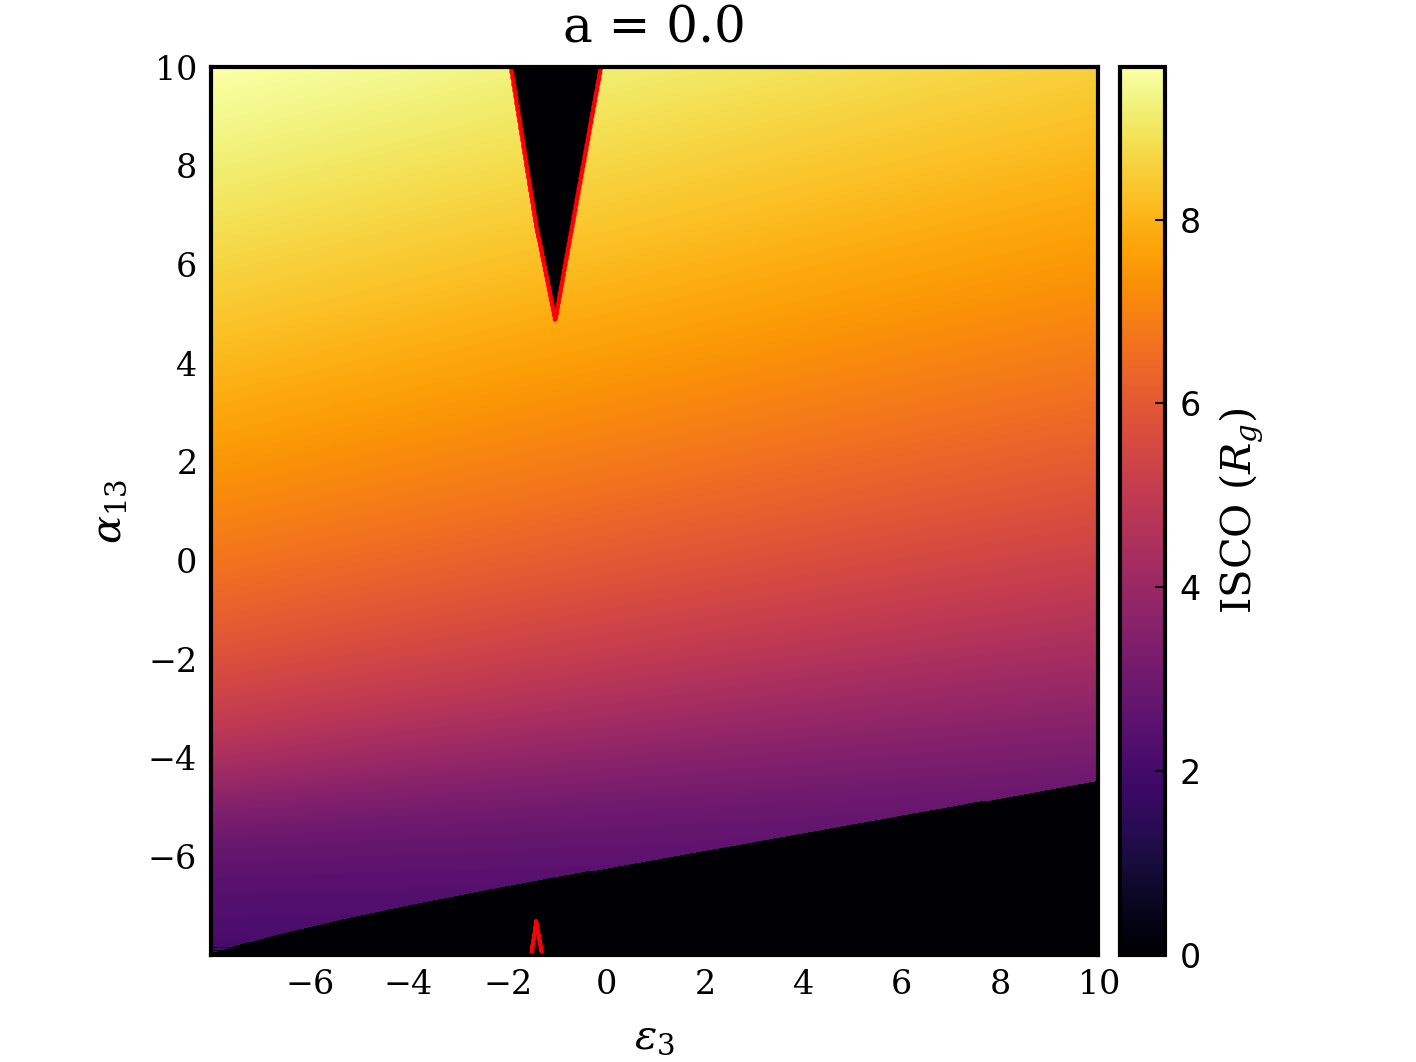
\includegraphics[keepaspectratio]{images/DeformParameterSpace_a=0.0.png}}

}

\caption{The valid deformation parameters for a Schwarszchild black
hole. The black regions show invalid configurations, and the red
contours denote regions where there is a naked singularity.}

\end{figure}%

Doing several of these plots for different values of the spin parameter
may permit rigorous constraints of the allowed values of the deformation
parameters. This may be done in two ways:

\begin{enumerate}
\def\labelenumi{\arabic{enumi}.}
\tightlist
\item
  Fitting the data with the Kerr metric to constrain the value of \(a\)
  such that bounds can be determined for the deformation parameters in
  advance.
\item
  Somehow dynamically setting constraints on the parameters by selecting
  from a pre-computed table of allowed combinations for all values of
  \(a\) (permitted by interpolation).
\item
  Checking the configuration upon each iteration of the fit, and either
  rejecting the configuration, or manually setting it to an acceptable
  configuration if it lies within an unphysical region.
\end{enumerate}

The first method would allow for an exploration as to whether the
deformation parameters can independently improve the fit of the model,
but may reduce the accuracy of the overall fit through forbidding the
spin parameter to change. This may be overcome by using the method to
obtain a ``best guess'' for the parameters and then using the result of
this for a third and final fit, however this may require implementing
the second method also.

The second method would likely be more computationally complex and
introduce an increased amount of uncertainty due to the reliance on
interpolation.

The third method is potentially the least complex and introduces the
least error as it allows the fit to freely explore the parameter space
while guiding it through the process to ensure the results remain
physical.

\section{The Behaviour of the Unphysical
Regions}\label{the-behaviour-of-the-unphysical-regions}

To gather more data on the allowed parameter space, the above image was
replicated for 5 spin values as shown below:

\begin{figure}

\begin{minipage}[t]{0.50\linewidth}

\raisebox{-\height}{

\pandocbounded{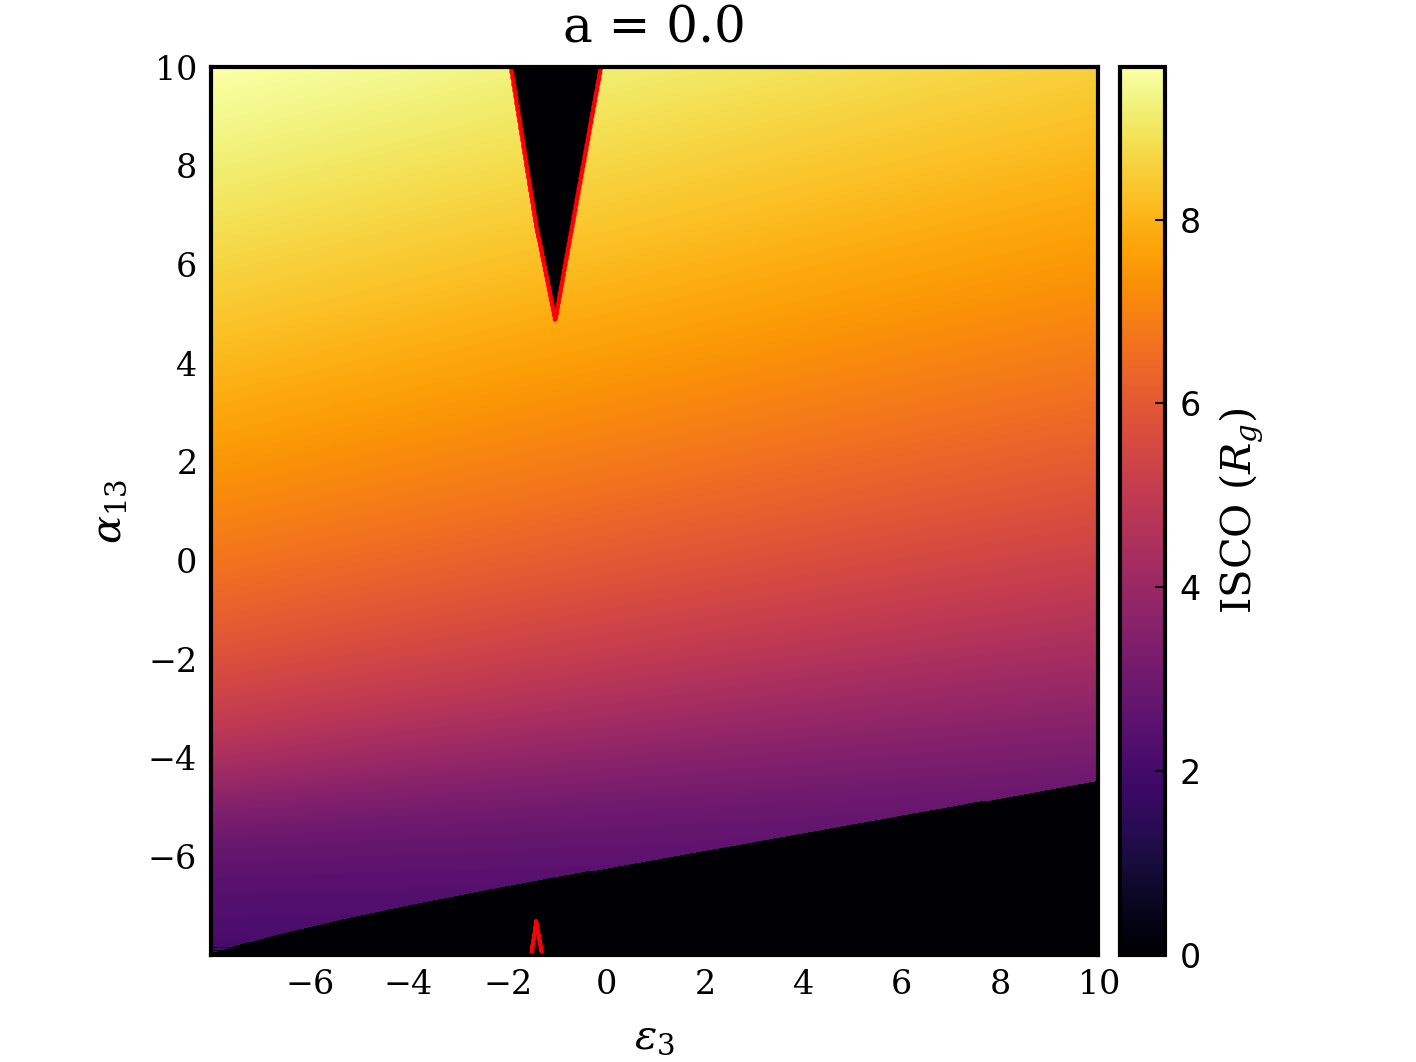
\includegraphics[keepaspectratio]{images/DeformParameterSpace_a=0.0.png}}

}

\end{minipage}%
%
\begin{minipage}[t]{0.50\linewidth}

\raisebox{-\height}{

\pandocbounded{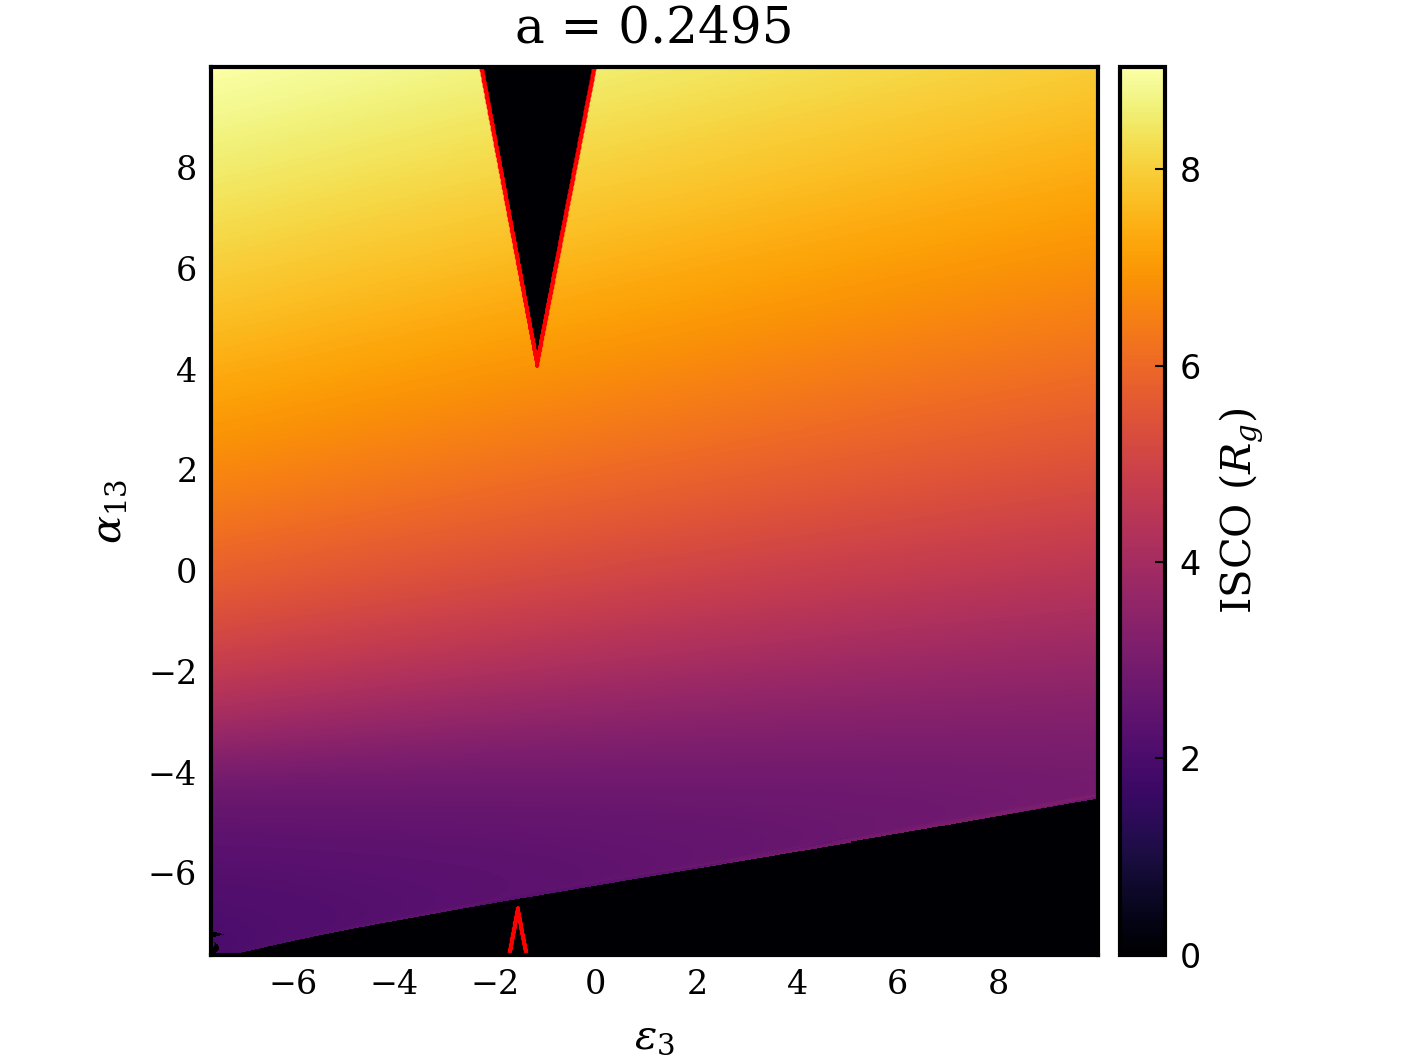
\includegraphics[keepaspectratio]{images/DeformParameterSpace_a=0.2495.png}}

}

\end{minipage}%
\newline
\begin{minipage}[t]{0.50\linewidth}

\raisebox{-\height}{

\pandocbounded{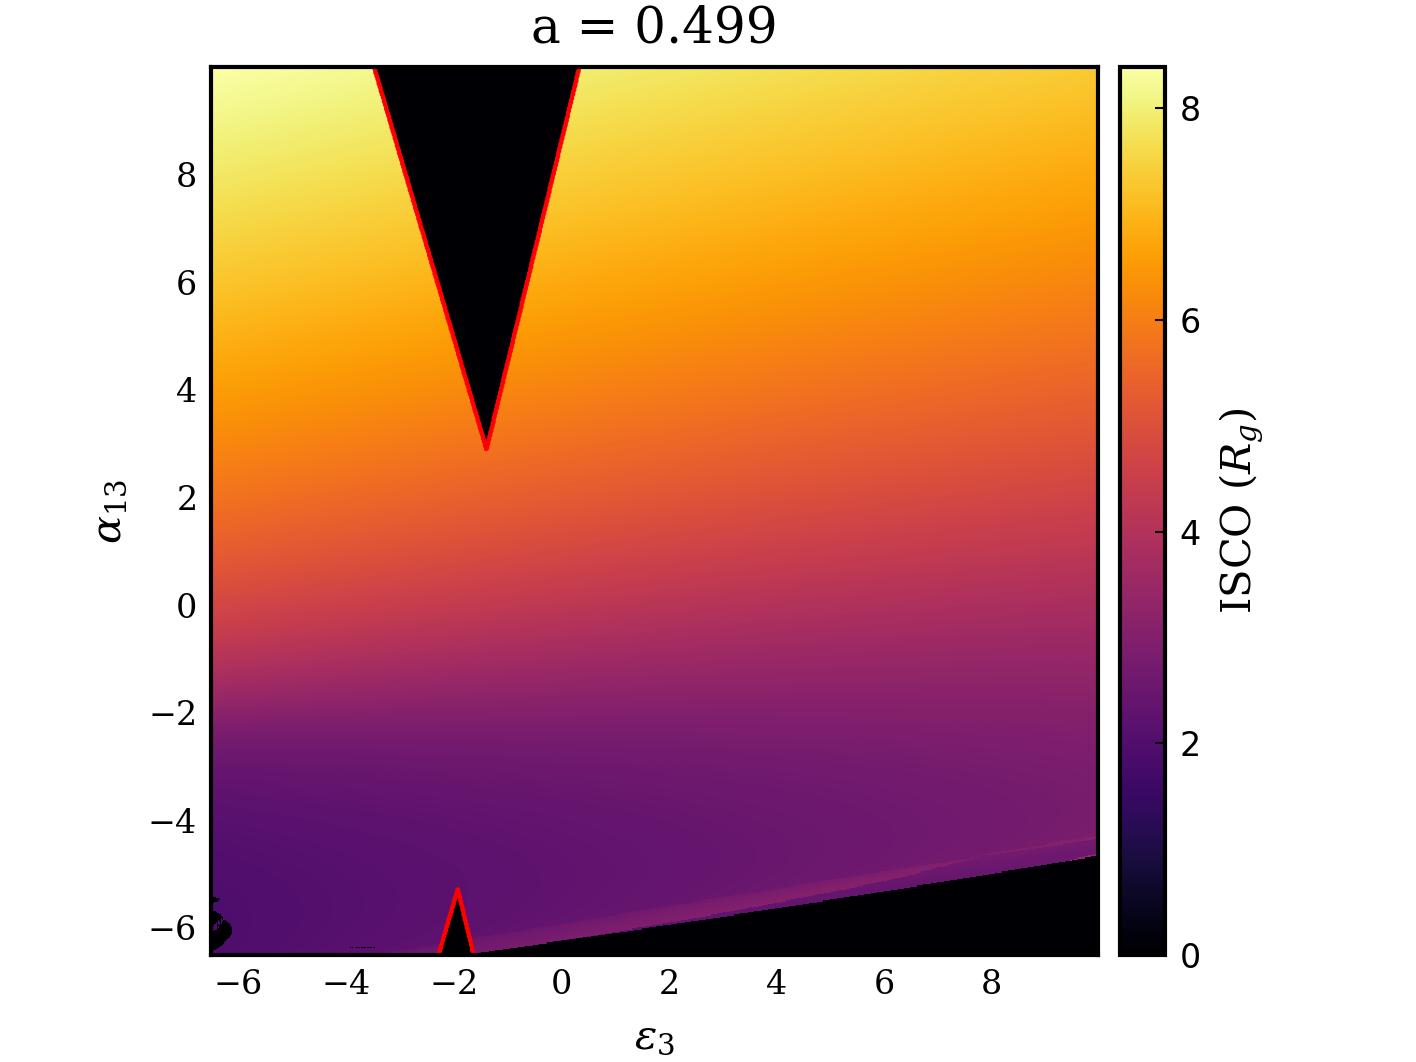
\includegraphics[keepaspectratio]{images/DeformParameterSpace_a=0.499.png}}

}

\end{minipage}%
%
\begin{minipage}[t]{0.50\linewidth}

\raisebox{-\height}{

\pandocbounded{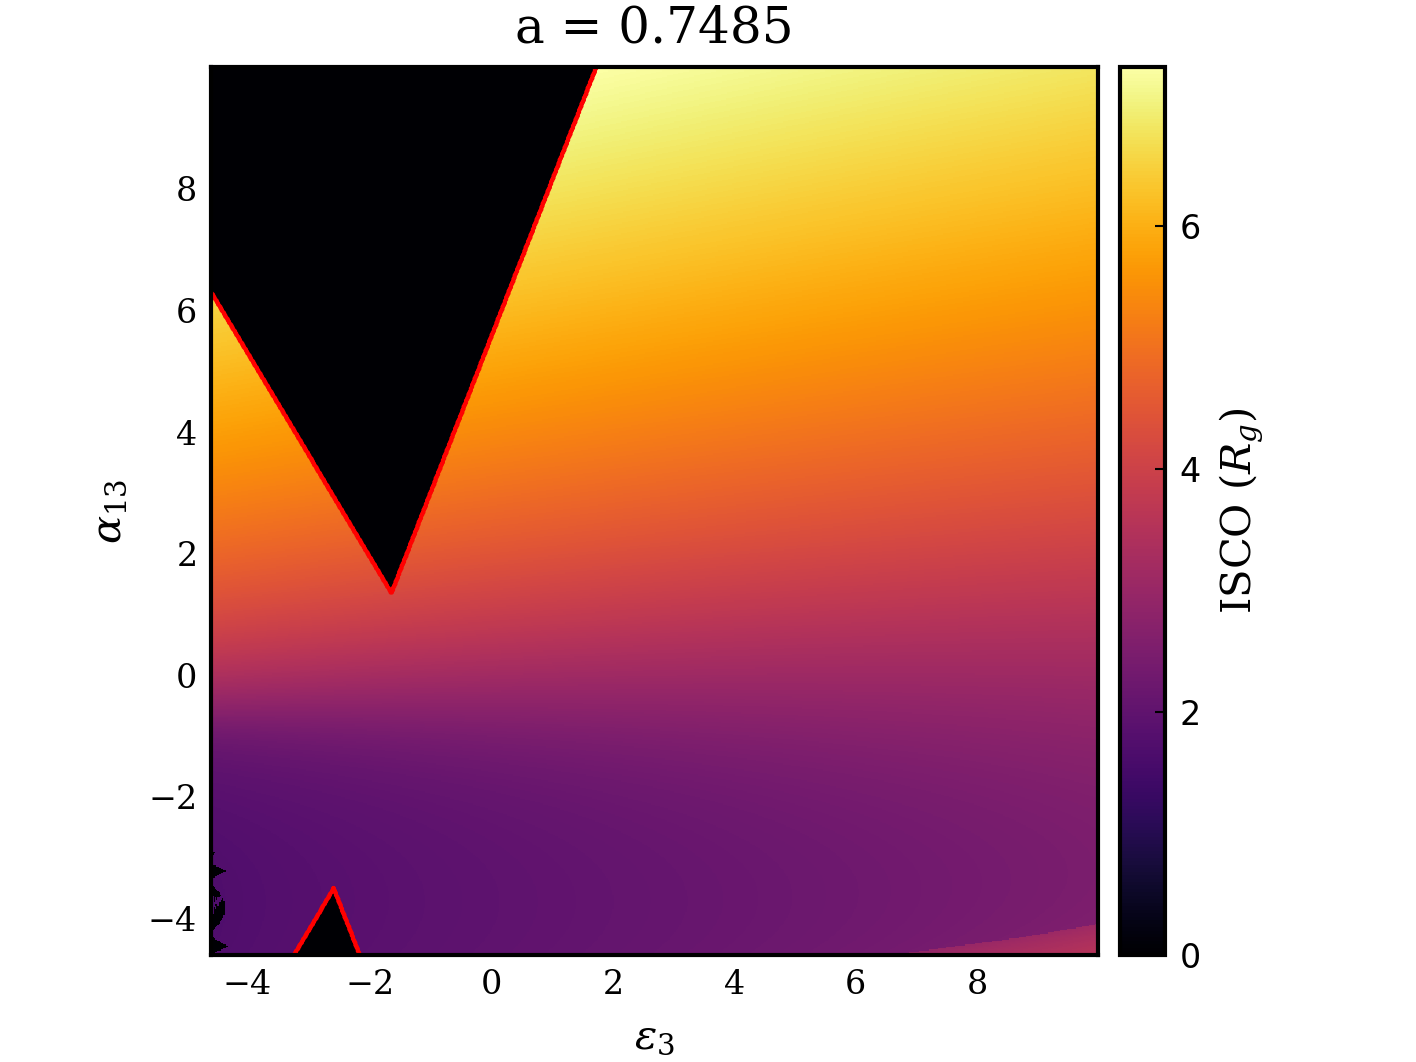
\includegraphics[keepaspectratio]{images/DeformParameterSpace_a=0.7485.png}}

}

\end{minipage}%
\newline
\begin{minipage}[t]{0.50\linewidth}

\raisebox{-\height}{

\pandocbounded{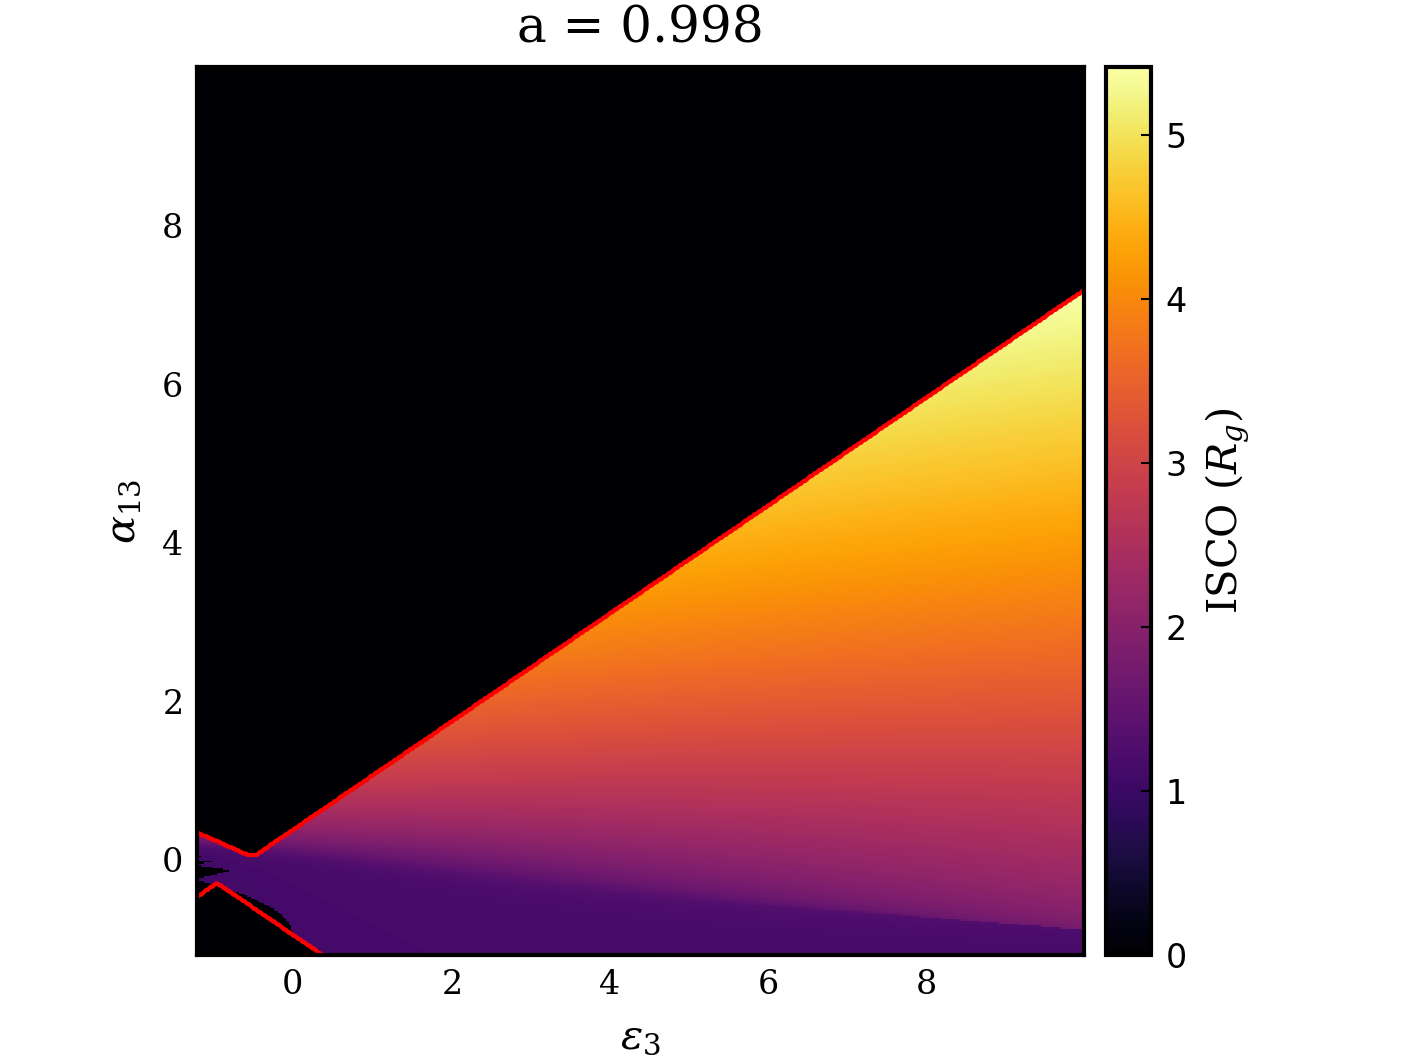
\includegraphics[keepaspectratio]{images/DeformParameterSpace_a=0.998.png}}

}

\end{minipage}%

\end{figure}%

From these plots it seems that it may be possible to empirically
parameterise the invalid regions with 5 linear equations: one for the
wedge in the bottom right first 3 figures, and two for each of the
triangles visible in all cases.

It may be practical to run a selection of cases to find the vertices of
these regions such that their position can be plotted as a function of
\(a\) and then fit to find an empirical expression for the allowed
values for any \(a\).

To test this hypothesis a quick plot was made with 10 samples of the
lower vertex of the triangular region seen in all plots at the top. The
result of this is shown below

\pandocbounded{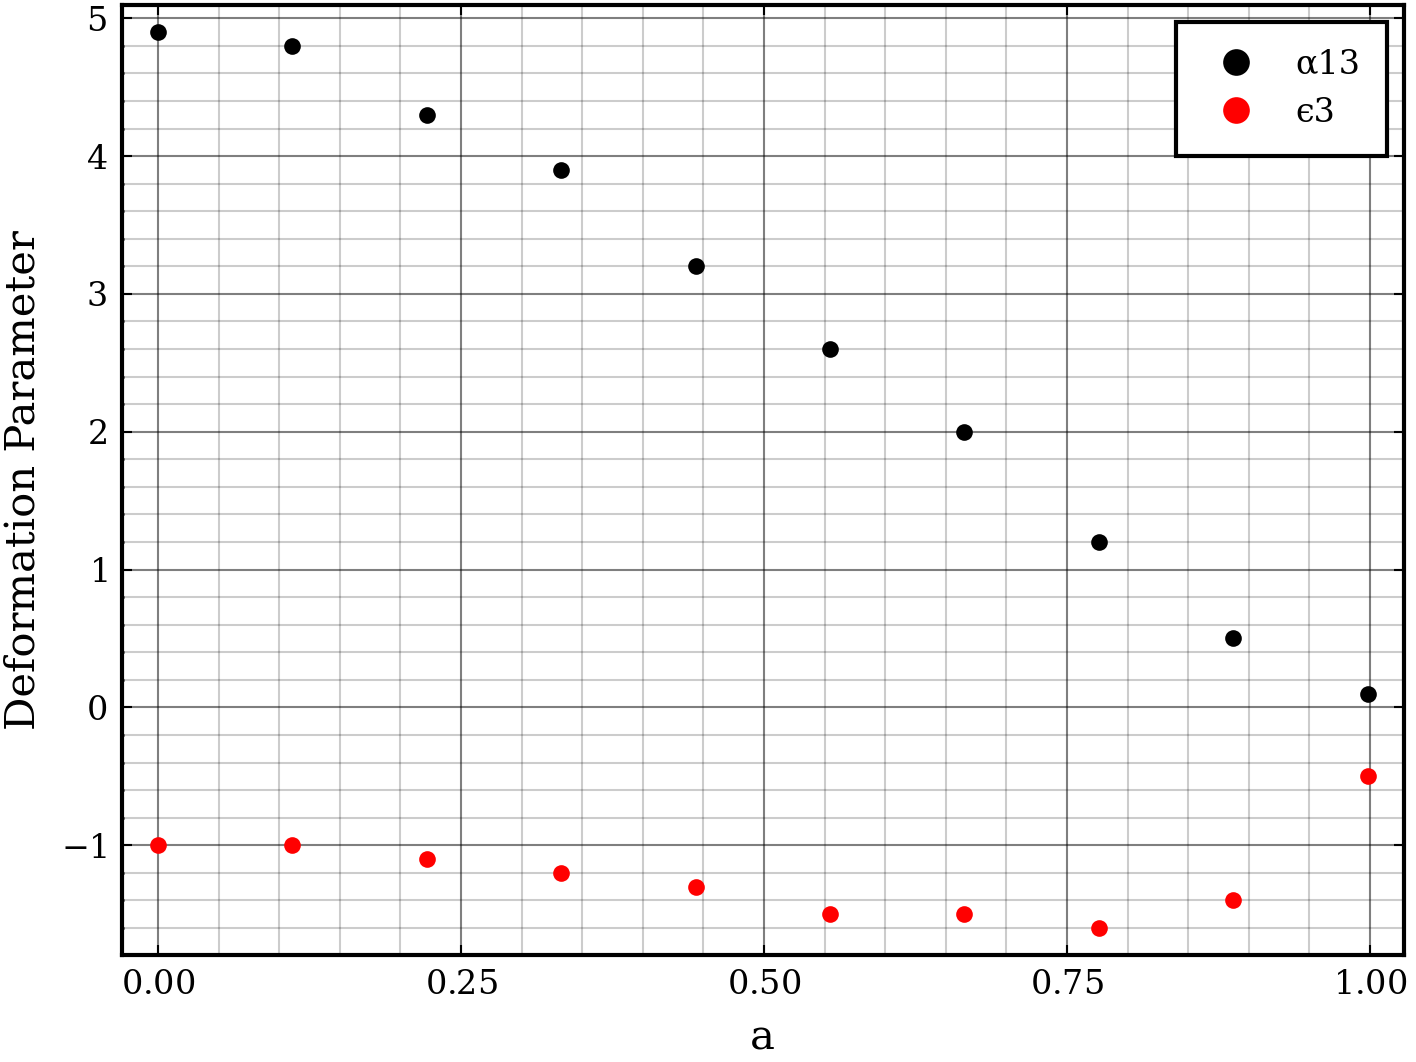
\includegraphics[keepaspectratio]{images/ParamBounds.png}}

These example coordinates were found manually inspecting the heatmap
with plotly. To find them more precisely, several high definition
heatmaps could be produced and the resulting matrix iterated through to
find the extrema of each of the shapes. The parameter space could then
be constrained by either interpolating the values within a table, or by
fitting some function to the data and finding the vertices of these
major shapes.

The vertices can then be used to define bounded exclusion regions,
within which the model is invalid. During fitting these exclusion
regions can then be used to ``reject'' a fit and force the parameters
into an acceptable range.

\section{Allowed Values of the Deformation Parameters for Varying
Spin}\label{allowed-values-of-the-deformation-parameters-for-varying-spin}

As another investigative route, Figure 6 from ~{[}3{]} was reproduced as
below. It was found that the results held consistent between Gradus, and
Johannsen's original calculations. The \(\alpha_{13}\) parameter space
showed an additional region (shown in red) where a naked singularity is
present. This was not considered previously, however removes a
significant region from the parameter space and will thus be considered
here.

\begin{figure}[H]

{\centering \pandocbounded{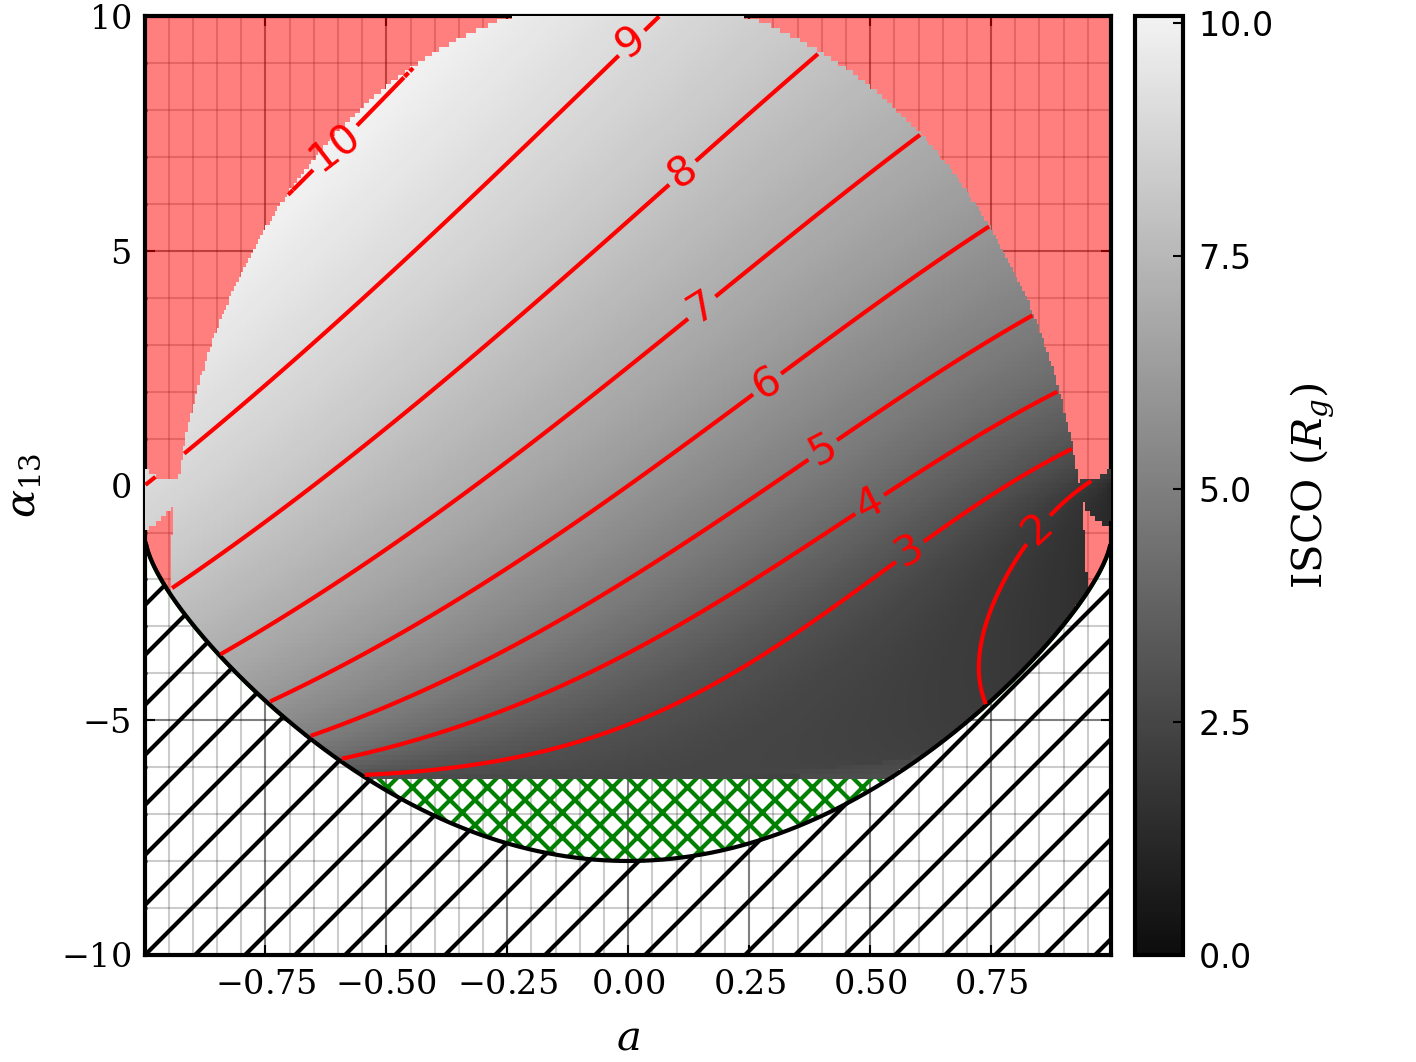
\includegraphics[keepaspectratio]{images/alpha13Allowed.png}}

}

\caption{The valid values for \(\epsilon_{3}\) to take for a range of
spin values. The black hatched region marks the constraints placed by
Equation~\ref{eq-Alpha13Constraint}. Contours of constant ISCO are
marked in red. The shaded red region marks where a naked singularity
occurs.}

\end{figure}%

\begin{figure}[H]

{\centering \pandocbounded{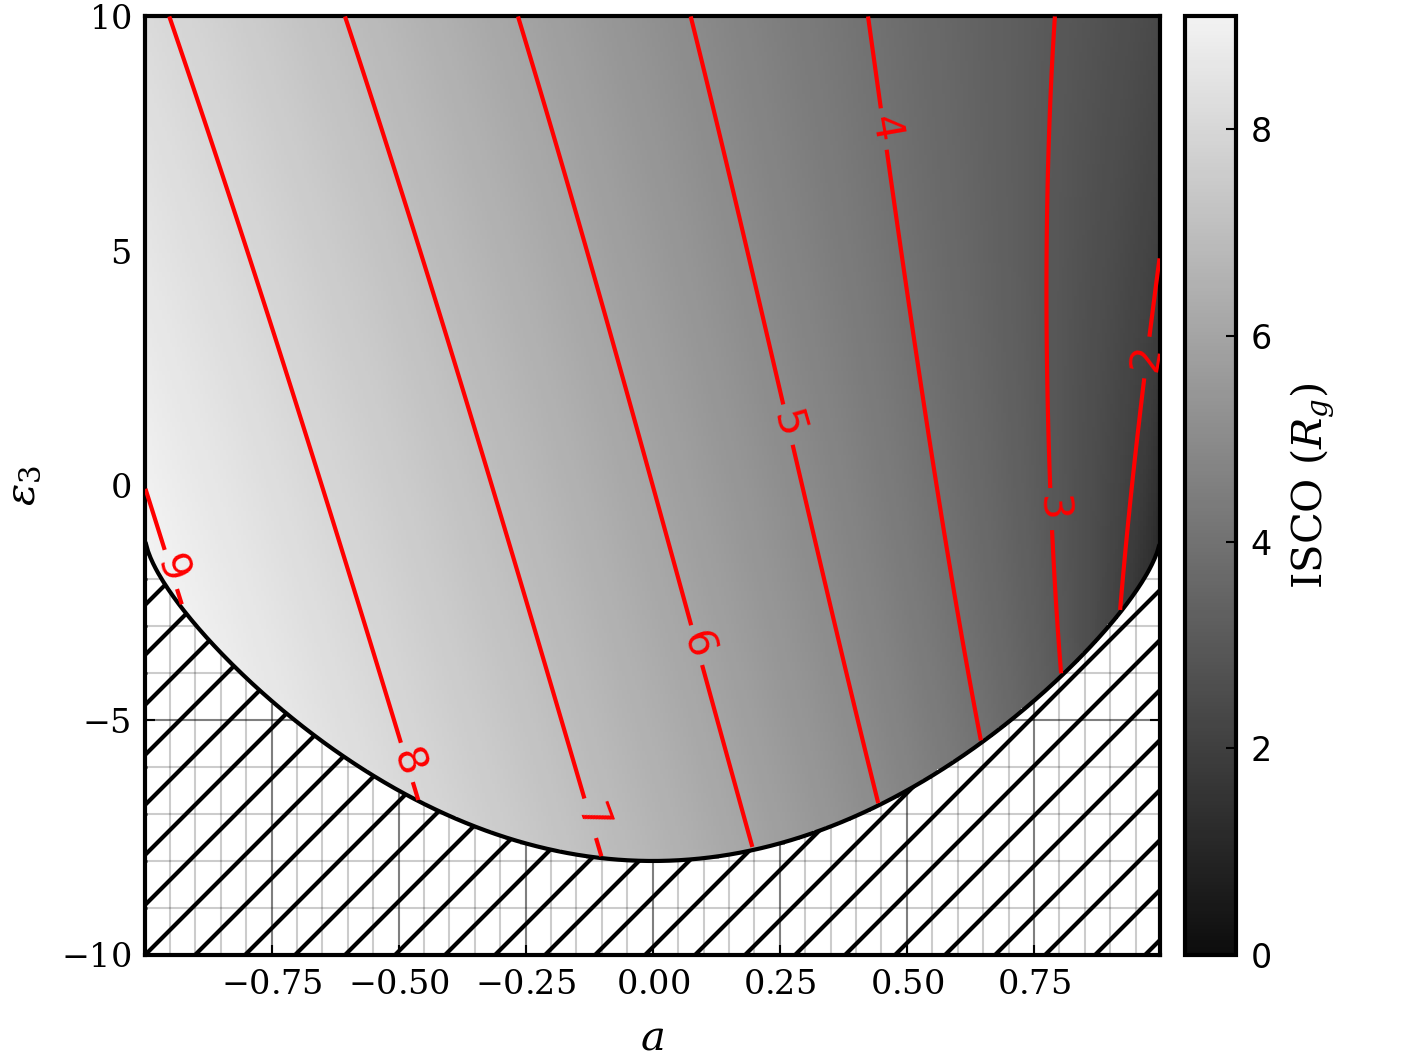
\includegraphics[keepaspectratio]{images/epsilon3Allowed.png}}

}

\caption{The valid values for \(\epsilon_{3}\) to take for a range of
spin values. The black hatched region marks the constraints placed by
Equation~\ref{eq-Epsilon3Constraint}. Contours of constant ISCO are
marked in red.}

\end{figure}%

\section{Implementation}\label{implementation}

\subsection{Plan 2026/07/10}\label{plan-20260710}

The current plan for excluding these unphysical regions of the parameter
space from the fitting is as follows. The unphysical regions will be
defined by a set of equations for a given spin, and within these regions
the fit will be setup to check if the combination is valid. To ensure no
invalid combinations are mistakenly used, some padding will be added to
these equations such that all invalid combinations are contained within.
When the fitting iterator enters an invalid region, the combination will
be explicitly checked for naked singularities, or the absence of a valid
ISCO.

If the region is found to be invalid, then the \texttt{invoke!} function
will return an array of zeros, which will signal to the fitting iterator
that the parameter combination is not allowed for fitting.

A potential roadblock to this process is the unpredictable region in the
bottom left corner of the high spin case. This will be dealt with by
defining a circular region around this area to catch all of these cases.
This will lead to a decrease in efficiency, but will increase the
accuracy and thoroughness of the model.

\subsection{Notes Following
Implementation}\label{notes-following-implementation}

The boundary lines were successfully defined by finding the vertices
through a grid search defined in \texttt{Code/utils/DeformUtils.jl}, and
a csv of gradients and intercepts was defined for quick reading of the
lines. Padding was added manually to these lines by randomly sampling
the parameter space and checking the validity of the combination both
using the bounds and explicitly checking the metric. Whenever the bounds
missed an invalid point in the parameter space they were adjusted
slightly and the process repeated until \(10^6\) consecutive random
samples could be taken without a point being missed. The bounds were
designed to be overzealous such that no valid combinations are missed.

To avoid removing valid combinations, the fitting process will involve
first a quick check with the boundaries, followed by a thorough check
with the metric if the first check fails.

The ``unpredictable region'' noted in the lower left corner was bounded
with a line rather than a circle for simplicity.

The call to the bounds within the fitting iterator is shown below

\begin{Shaded}
\begin{Highlighting}[]
\CommentTok{\# Reading from table for a quick check of parameter validity}
\ControlFlowTok{if}\NormalTok{ !}\FunctionTok{QuickIsValid}\NormalTok{(ϵ}\FloatTok{3}\NormalTok{, α}\FloatTok{13}\NormalTok{, a)}
    \CommentTok{\# Doing a finer check if the quick check fails}
    \ControlFlowTok{if}\NormalTok{ !}\FunctionTok{IsValid}\NormalTok{(ϵ}\FloatTok{3}\NormalTok{, α}\FloatTok{13}\NormalTok{, a)}
\NormalTok{        output }\OperatorTok{=} \FunctionTok{fill}\NormalTok{(}\ConstantTok{NaN}\NormalTok{, }\FunctionTok{length}\NormalTok{(input)}\OperatorTok{{-}}\FloatTok{1}\NormalTok{)}
        \ControlFlowTok{return}\NormalTok{ output}
    \ControlFlowTok{end}
\ControlFlowTok{end}
\end{Highlighting}
\end{Shaded}

Here \texttt{QuickIsValid} checks the combination using the defined
bounds and \texttt{IsValid} checks it thoroughly using the metric
through \texttt{Gradus.jl}. If both checks find the parameter
combination to be invalid then the model returns an array of
\texttt{NaN} for that iteration, such that the iterator will calculate a
bad fit and move out of the region. The conditions that are checked
through these functions are:

\begin{itemize}
\tightlist
\item
  The presence of a valid ISCO: Checked by defining a metric through
  \texttt{Gradus.jl} and attempting to calculate the isco using
  \texttt{Gradus.ISCO}
\item
  The presence of a naked singularity: Checked using
  \texttt{Gradus.is\_naked\_singularity}
\item
  If the combination satisfies Equation~\ref{eq-Alpha13Constraint} and
  Equation~\ref{eq-Epsilon3Constraint}
\item
  If the magnitude of the spin is below 0.998
\end{itemize}

The final check is done as the fitting iterator sometimes exceeds the
upper limit, causing the interpolation for the bound definitions to try
to extrapolate which causes errors.

The next step is to create a final table model to use for the fit that
covers the entire allowed parameter space. In the construction of this,
each combination will be checked for a valid ISCO and if
Equation~\ref{eq-Alpha13Constraint} and
Equation~\ref{eq-Epsilon3Constraint} are satisfied. If any of these are
not satisfied then that point in the table will be an array of
\texttt{NaN} to ensure that it does not get used.

\begin{figure}[H]

{\centering \pandocbounded{\includegraphics[keepaspectratio]{images/Bounds.gif}}

}

\caption{The bounds (shown by the dotted regions) and the invalid
regions (shown by the solid regions). The grey regions are where there
is no valid ISCO, and the black regions are where there is a naked
singularity}

\end{figure}%

\subsection{2026/07/17}\label{section}

The previous suggested method of constructing the table model did not
work due to the fact that the interpolator attempted to use the regions
set to \texttt{NaN}, producing invalid spectra where there should not
have been. Thus a new method was devised where rather than setting the
spectra for the invalid regions to an array of \texttt{NaN} it would be
set to a spectrum calculated from the closest valid point in the
parameter space. This would increase the uncertainty in the results from
the table model, which must be quantified by comparing the results from
\texttt{Gradus} and the table model.

To implement this, the table for \texttt{QuickIsValid} was refined such
that the boundaries fit as close as possible to the invalid regions.
This refinement was done by gradually increasing the number of rows of
the table through interpolating and adjusting the gradients and
intercepts for the 6 lines manually. A function was then defined to
first find what invalid region a point is in, then define a line from
the point perpendicular to the boundary. The intersection between this
line and the boundary then gives the new point to move to in parameter
space.

This was then implemented into the construction of the table model by
adjusting the deformation parameters whenever they are invalid, which
will provide valid spectra, albeit likely at the cost of accuracy.

\subsection{2026/07/21}\label{section-1}

After implementing this it was found that some parameter combinations
still failed to compute, or took an unreasonable amount of time to
compute. Attempts to fix this included

\begin{enumerate}
\def\labelenumi{\arabic{enumi}.}
\tightlist
\item
  Using different solvers that work for stiff equations as suggested by
  the warning raised by \texttt{DifferentialEquations.jl}
\end{enumerate}

\begin{verbatim}
┌ Warning: Verbosity toggle: max_iters 
│  Interrupted. Larger maxiters is needed. If you are using an integrator for non-stiff ODEs or an automatic switching algorithm (the default), you may want to consider using a method for stiff equations. See the solver pages for more details (e.g. https://docs.sciml.ai/DiffEqDocs/stable/solvers/ode_solve/#Stiff-Problems).
└ @ SciMLBase ~/.julia/packages/SciMLBase/O1HPI/src/integrator_interface.jl:679
\end{verbatim}

\begin{enumerate}
\def\labelenumi{\arabic{enumi}.}
\setcounter{enumi}{1}
\tightlist
\item
  Ensuring that the metric is valid, which was satisfied for all test
  cases.
\item
  Moving the lamppost corona out of the ISCO if it was within it.
\item
  Using the \texttt{BinningMethod} dispatch to calculate the line
  profile.
\item
  Running the code on a different operating system (Windows 11).
\end{enumerate}

None of these fixed the issue, however it was later noticed that the
parameter combinations with negative spin were more prone to these
errors. In the interest of progressing with the investigations, it was
thus decided to only consider positive spin, i.e.~Prograde motion of the
accretion disk ~{[}9{]}.

\subsection{2026/07/22}\label{section-2}

A new interesting finding with regards to this issue: The failed
combinations seem to have consistently low \(\alpha_{13}\). A test was
ran with 1000 different combinations throughout the parameter space with
the following ranges:

\begin{verbatim}
as   = range(0, 0.998, 10)
α13s = range(-8., 10., 10)
ϵ3s  = range(-8., 10., 10)
\end{verbatim}

The following 15 combinations failed to compute

{\def\LTcaptype{none} % do not increment counter
\begin{longtable}[]{@{}lll@{}}
\toprule\noalign{}
\(a\) & \(\alpha_{13}\) & \(\epsilon_{3}\) \\
\midrule\noalign{}
\endhead
\bottomrule\noalign{}
\endlastfoot
0.33266666666666667 & -6.84 & -5.96 \\
0.6653333333333333 & -4.8 & -3.92 \\
0.5544444444444444 & -5.55 & -3.94 \\
0.6653333333333333 & -4.71 & -1.46 \\
0.5544444444444444 & -5.55 & -3.93 \\
0.7762222222222223 & -4.08 & -1.58 \\
0.8871111111111111 & -2.61 & 0.03 \\
0.998 & -1.02 & 6.09 \\
0.7762222222222223 & -4.23 & 0.1 \\
0.7762222222222223 & -4.2 & 2.1 \\
0.7762222222222223 & -3.92 & 4.05 \\
0.7762222222222223 & -3.81 & -1.72 \\
0.7762222222222223 & -4.0 & 0.0 \\
0.7762222222222223 & -4.0 & 2.0 \\
0.7762222222222223 & -3.9 & 4.1 \\
\end{longtable}
}

Plotted in parameter space, these combinations are placed as follows:

\begin{figure}

\begin{minipage}[t]{0.50\linewidth}
\begin{center}
\pandocbounded{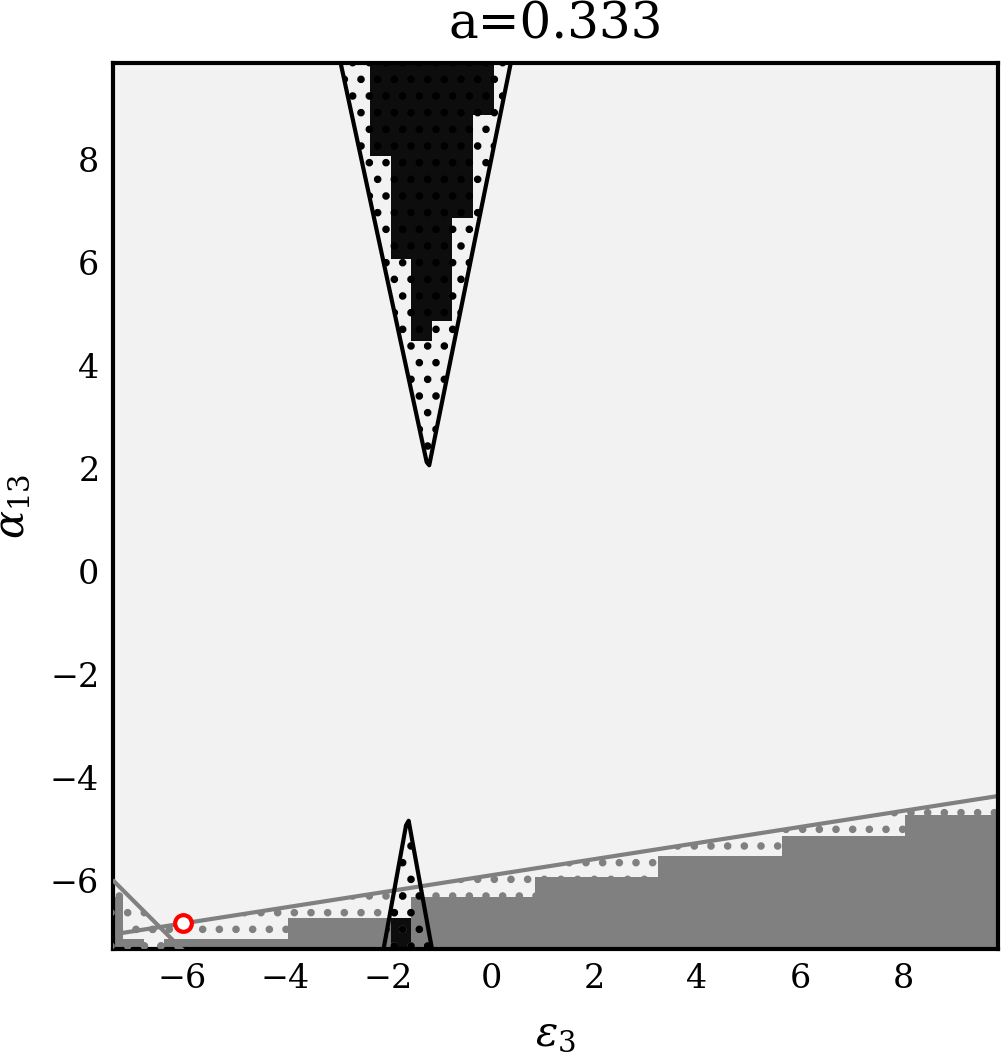
\includegraphics[keepaspectratio]{images/Fail1.png}}
\end{center}
\end{minipage}%
%
\begin{minipage}[t]{0.50\linewidth}
\begin{center}
\pandocbounded{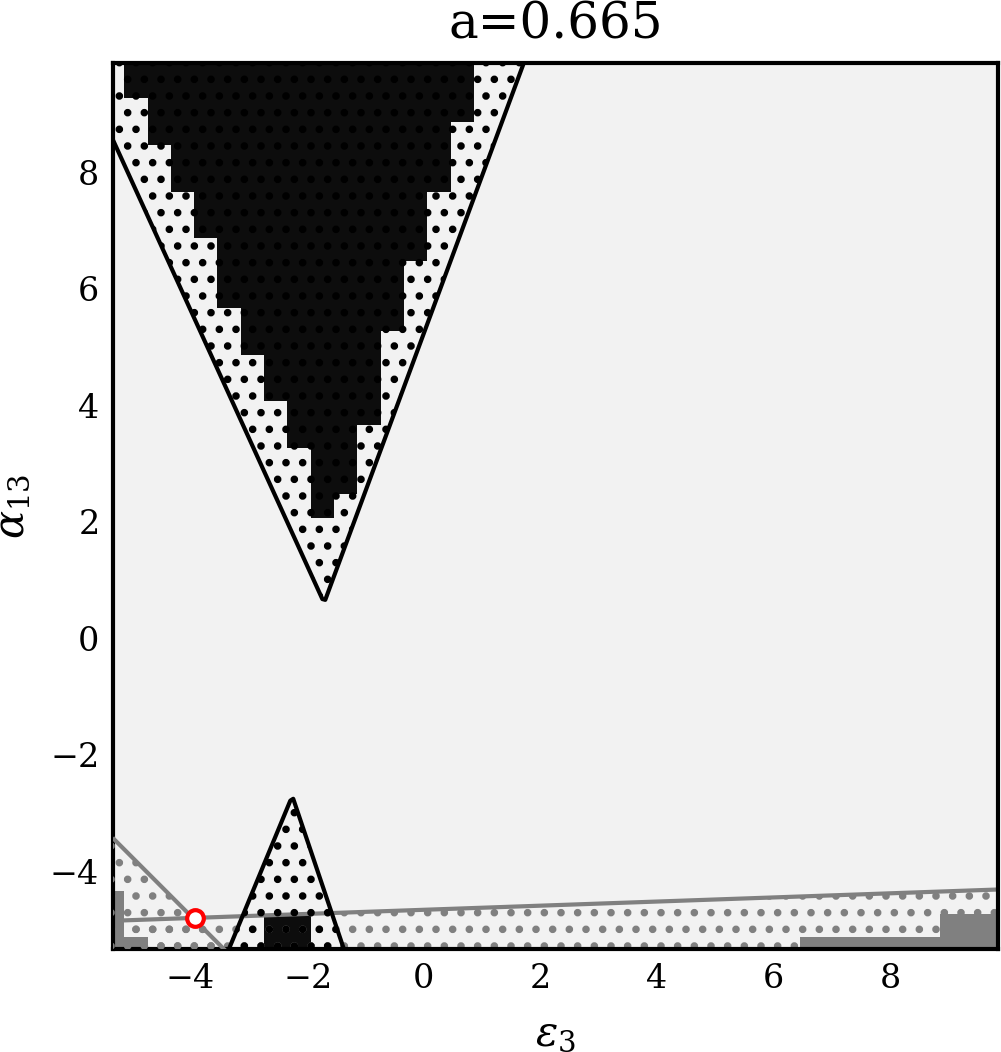
\includegraphics[keepaspectratio]{images/Fail2.png}}
\end{center}
\end{minipage}%
\newline
\begin{minipage}[t]{0.50\linewidth}
\begin{center}
\pandocbounded{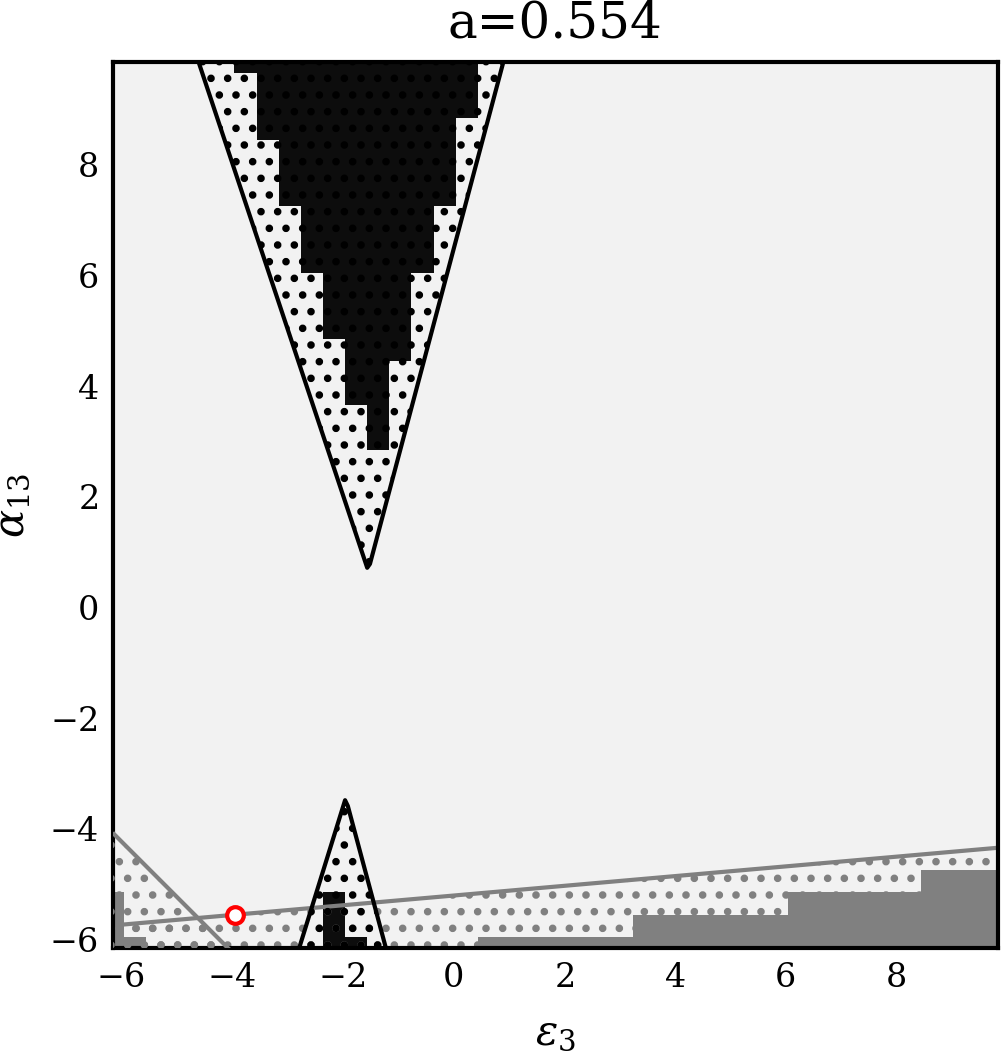
\includegraphics[keepaspectratio]{images/Fail3.png}}
\end{center}
\end{minipage}%
%
\begin{minipage}[t]{0.50\linewidth}
\begin{center}
\pandocbounded{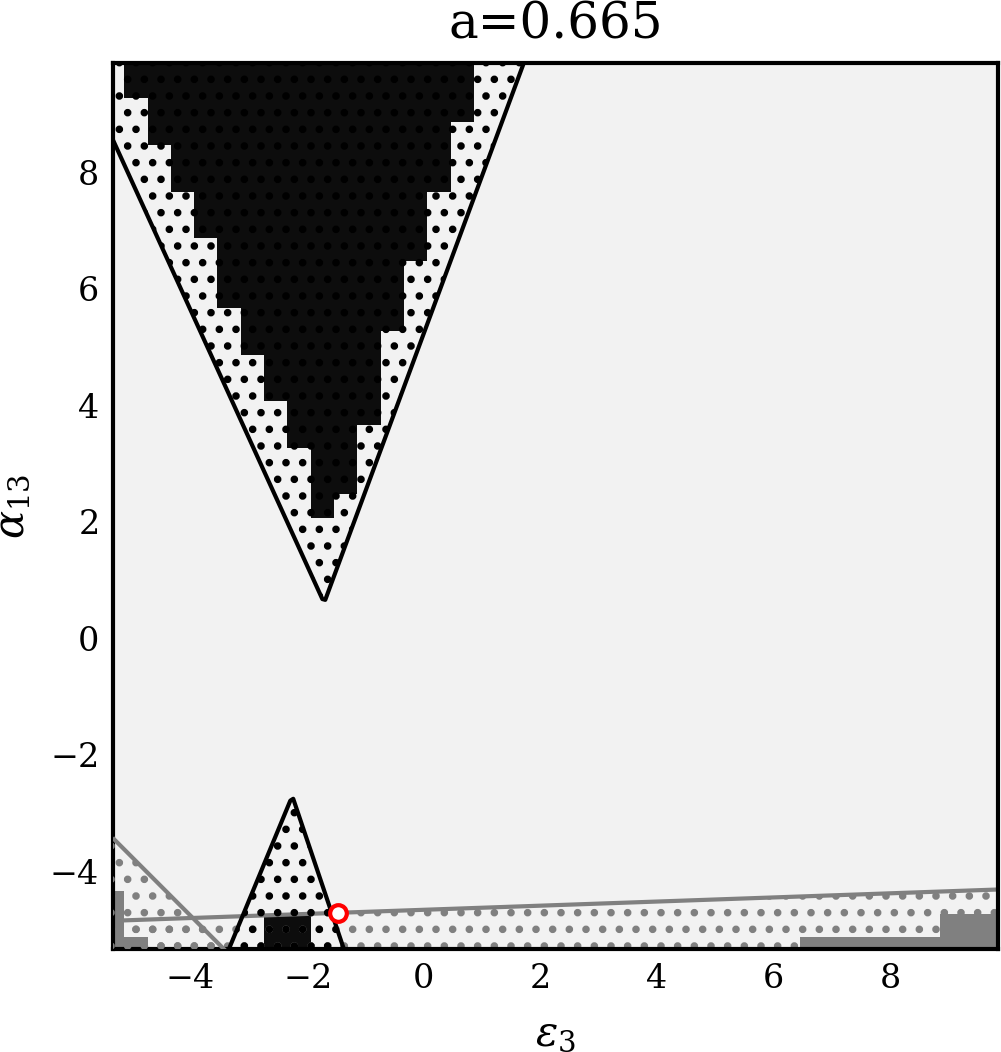
\includegraphics[keepaspectratio]{images/Fail4.png}}
\end{center}
\end{minipage}%
\newline
\begin{minipage}[t]{0.50\linewidth}
\begin{center}
\pandocbounded{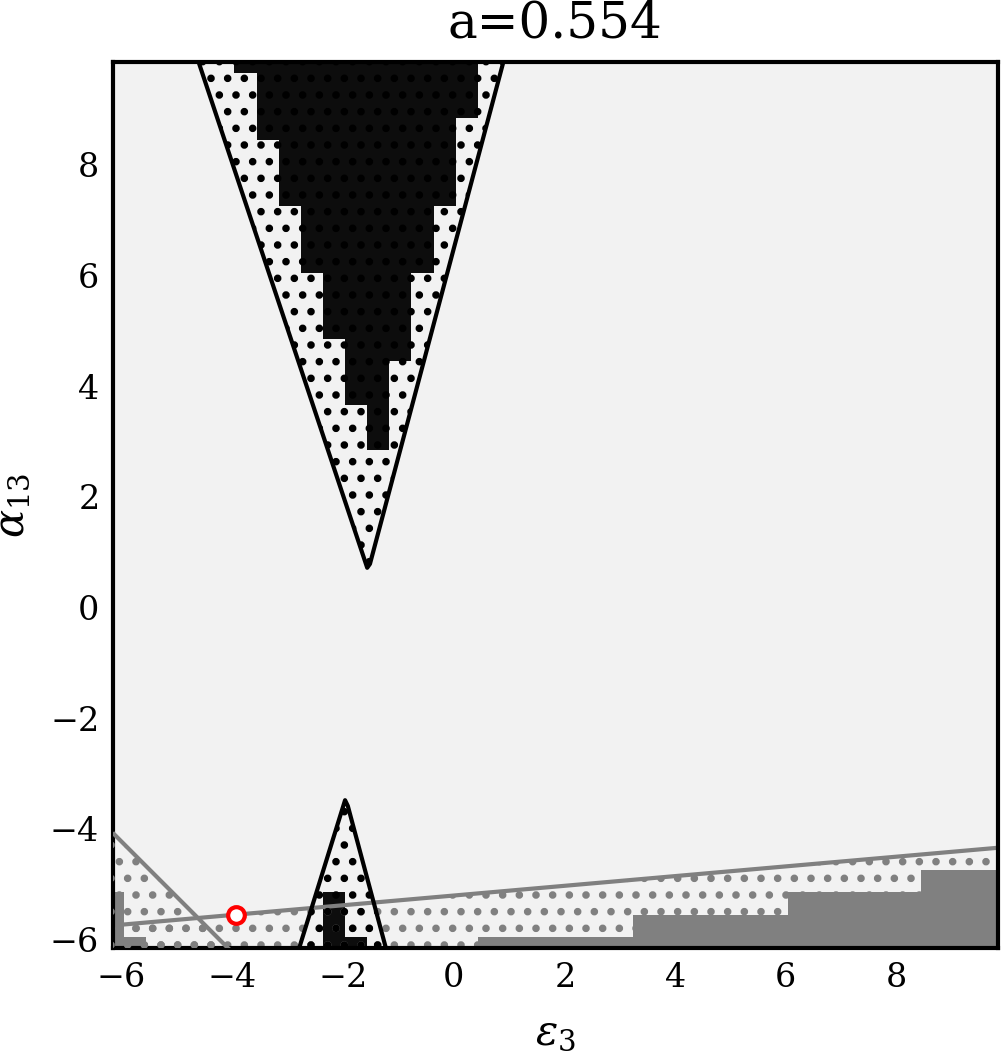
\includegraphics[keepaspectratio]{images/Fail5.png}}
\end{center}
\end{minipage}%
%
\begin{minipage}[t]{0.50\linewidth}
\begin{center}
\pandocbounded{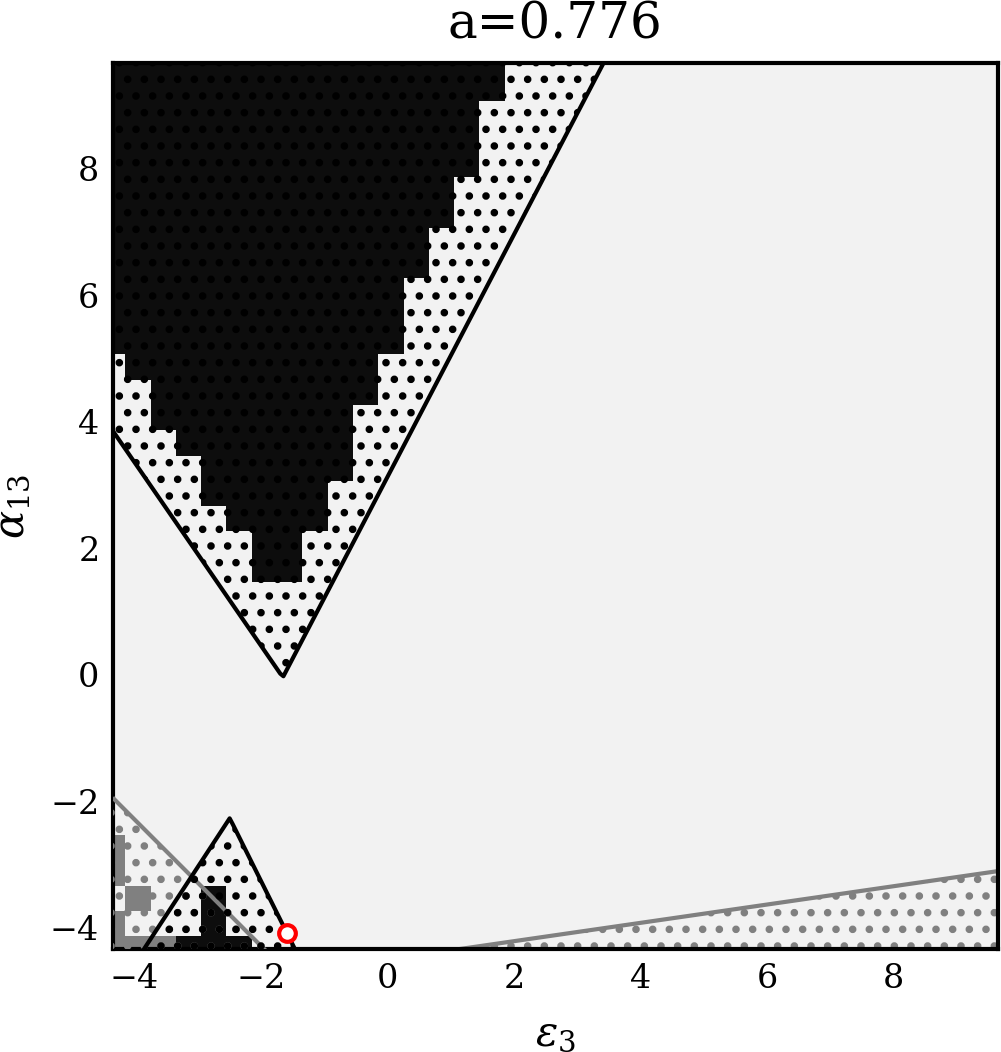
\includegraphics[keepaspectratio]{images/Fail6.png}}
\end{center}
\end{minipage}%
\newline
\begin{minipage}[t]{0.50\linewidth}
\begin{center}
\pandocbounded{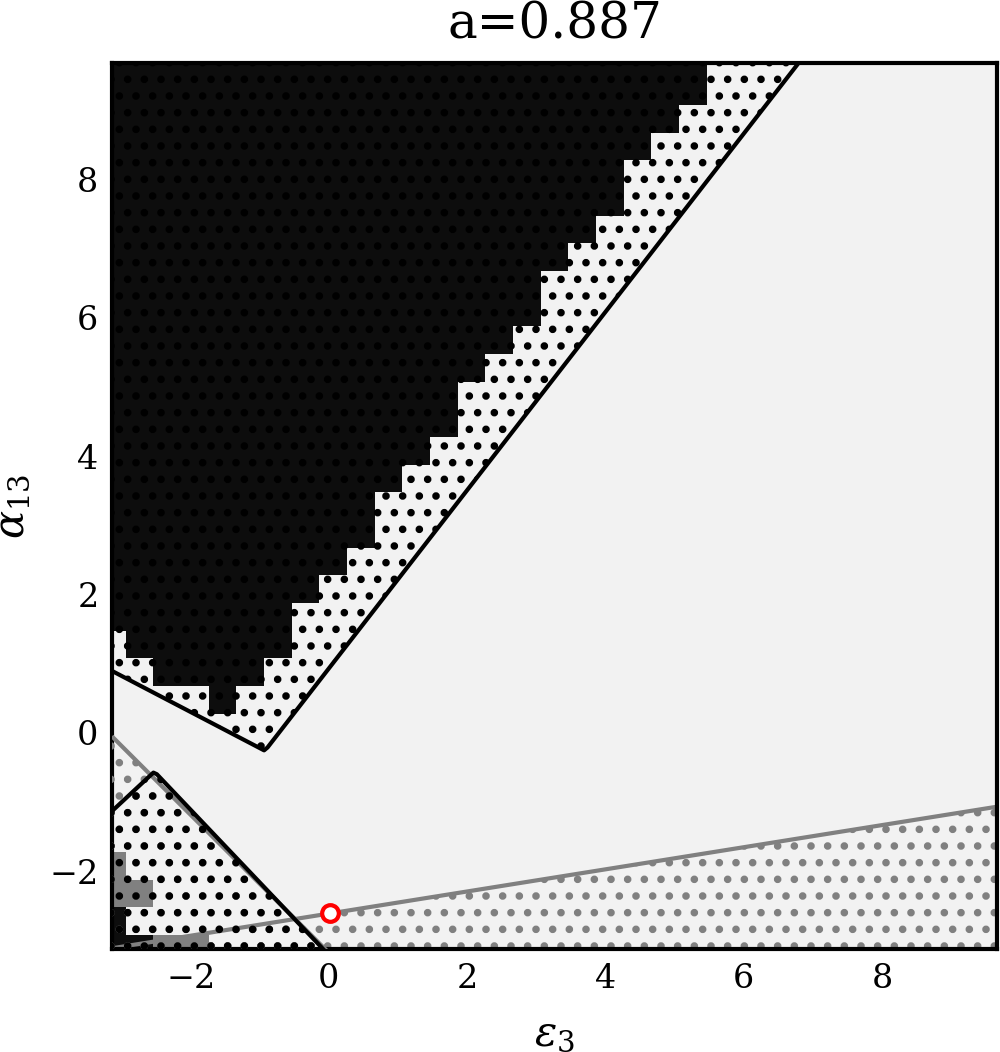
\includegraphics[keepaspectratio]{images/Fail7.png}}
\end{center}
\end{minipage}%
%
\begin{minipage}[t]{0.50\linewidth}
\begin{center}
\pandocbounded{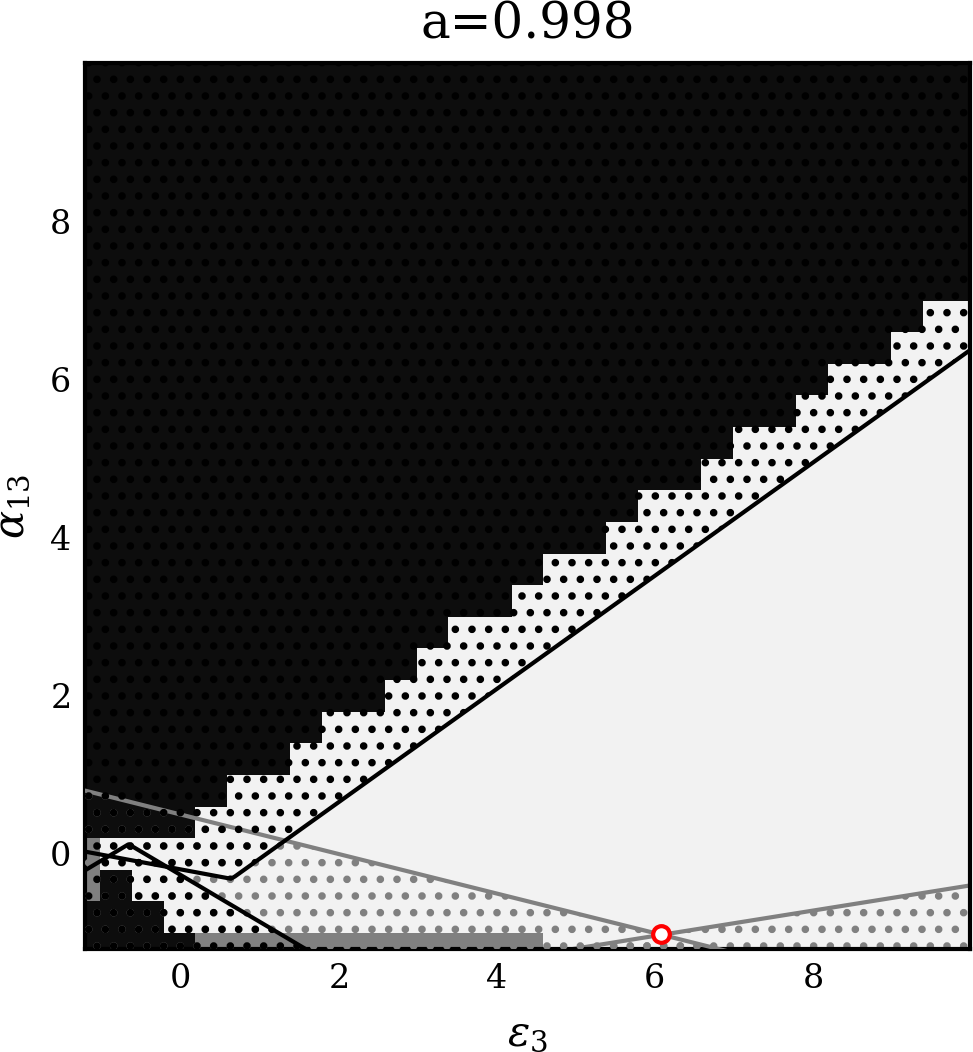
\includegraphics[keepaspectratio]{images/Fail8.png}}
\end{center}
\end{minipage}%
\newline
\begin{minipage}[t]{0.50\linewidth}
\begin{center}
\pandocbounded{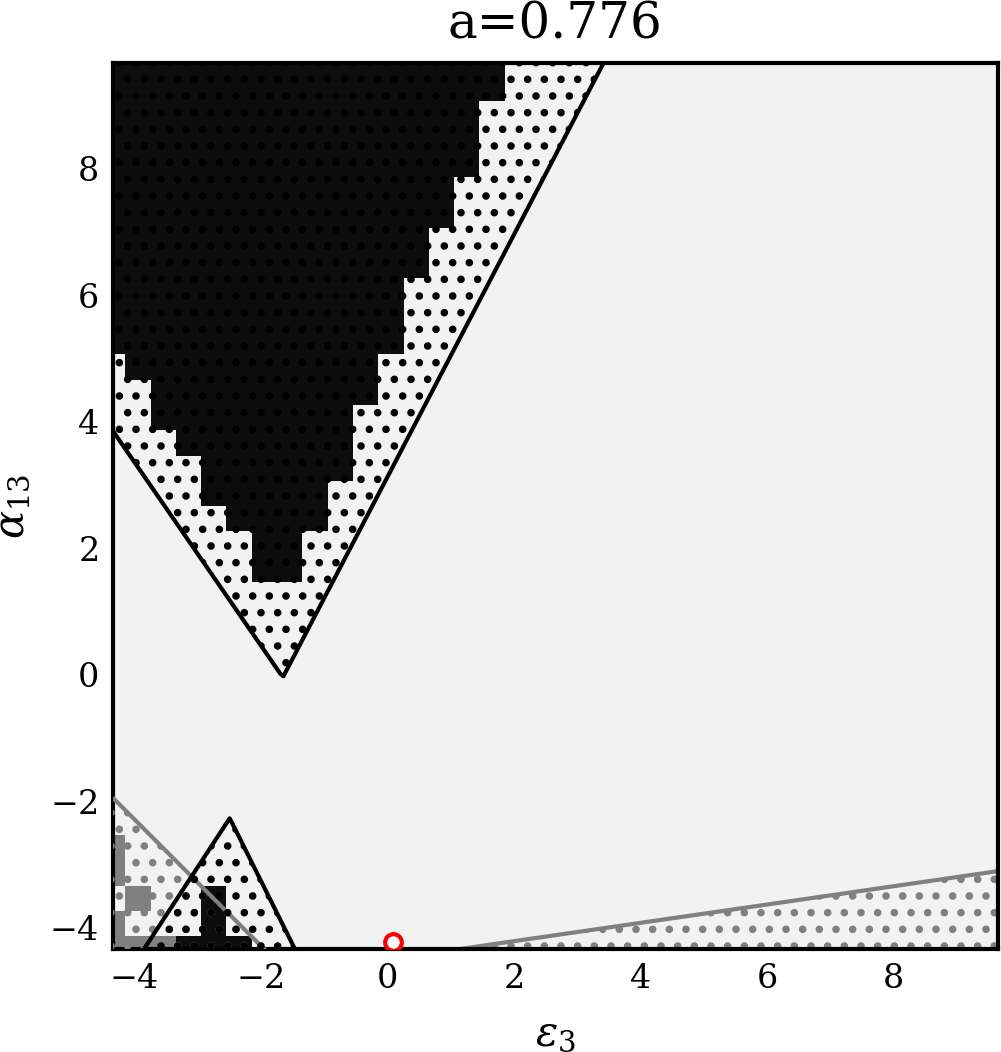
\includegraphics[keepaspectratio]{images/Fail9.png}}
\end{center}
\end{minipage}%
%
\begin{minipage}[t]{0.50\linewidth}
\begin{center}
\pandocbounded{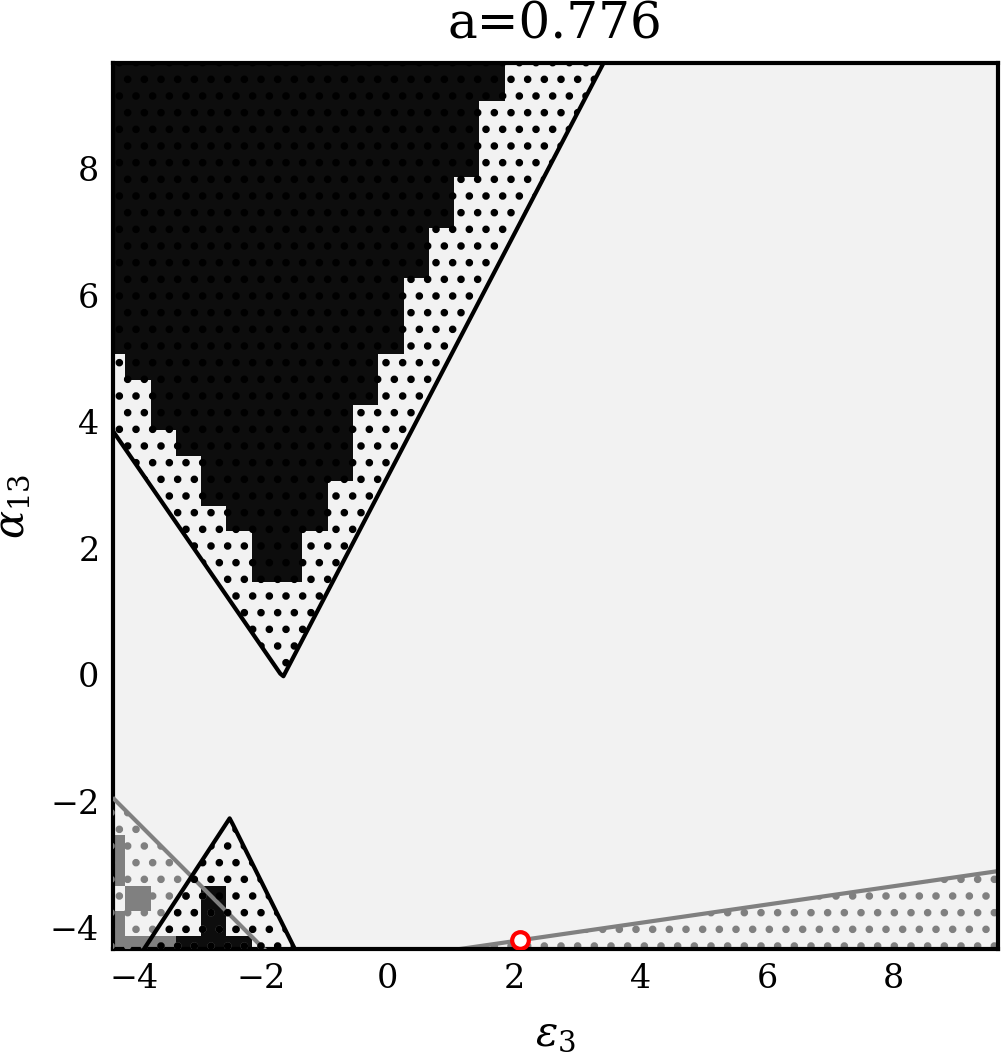
\includegraphics[keepaspectratio]{images/Fail10.png}}
\end{center}
\end{minipage}%
\newline
\begin{minipage}[t]{0.50\linewidth}
\begin{center}
\pandocbounded{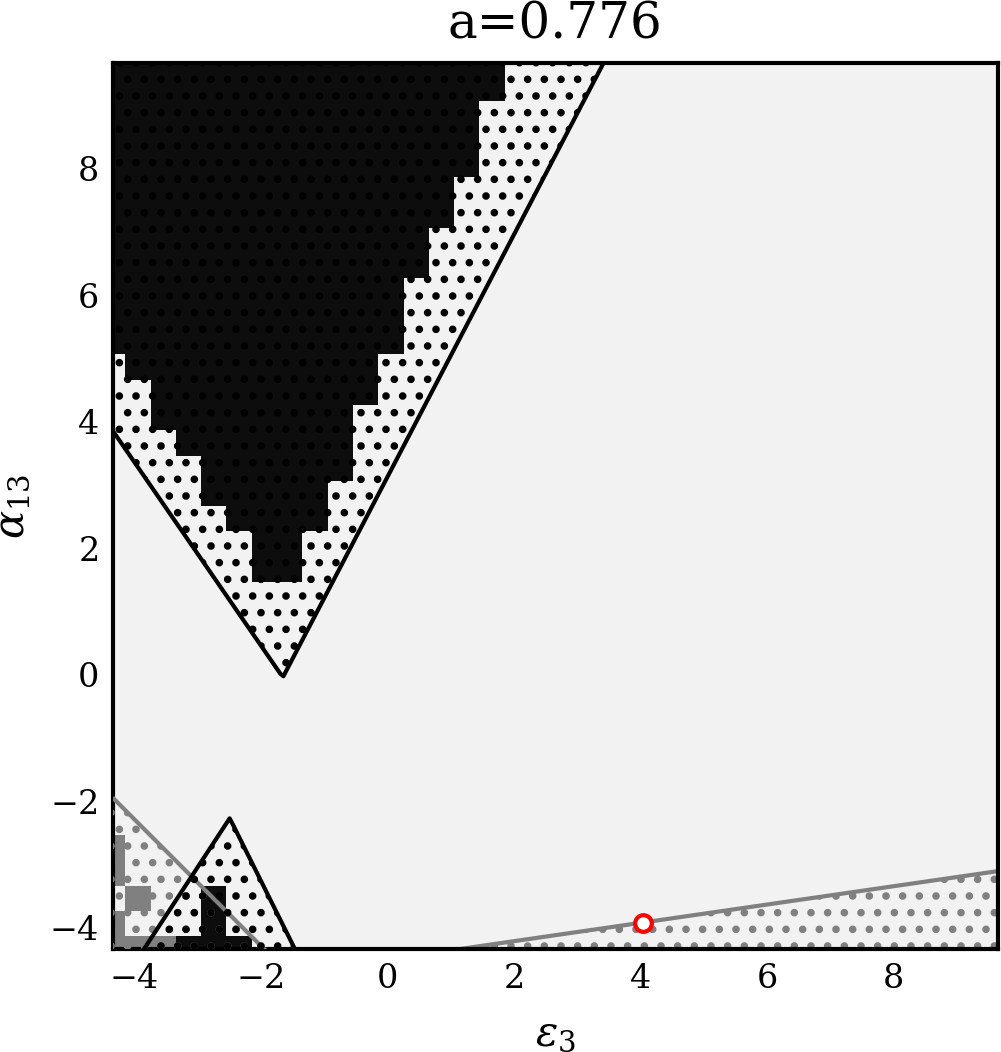
\includegraphics[keepaspectratio]{images/Fail11.png}}
\end{center}
\end{minipage}%
%
\begin{minipage}[t]{0.50\linewidth}
\begin{center}
\pandocbounded{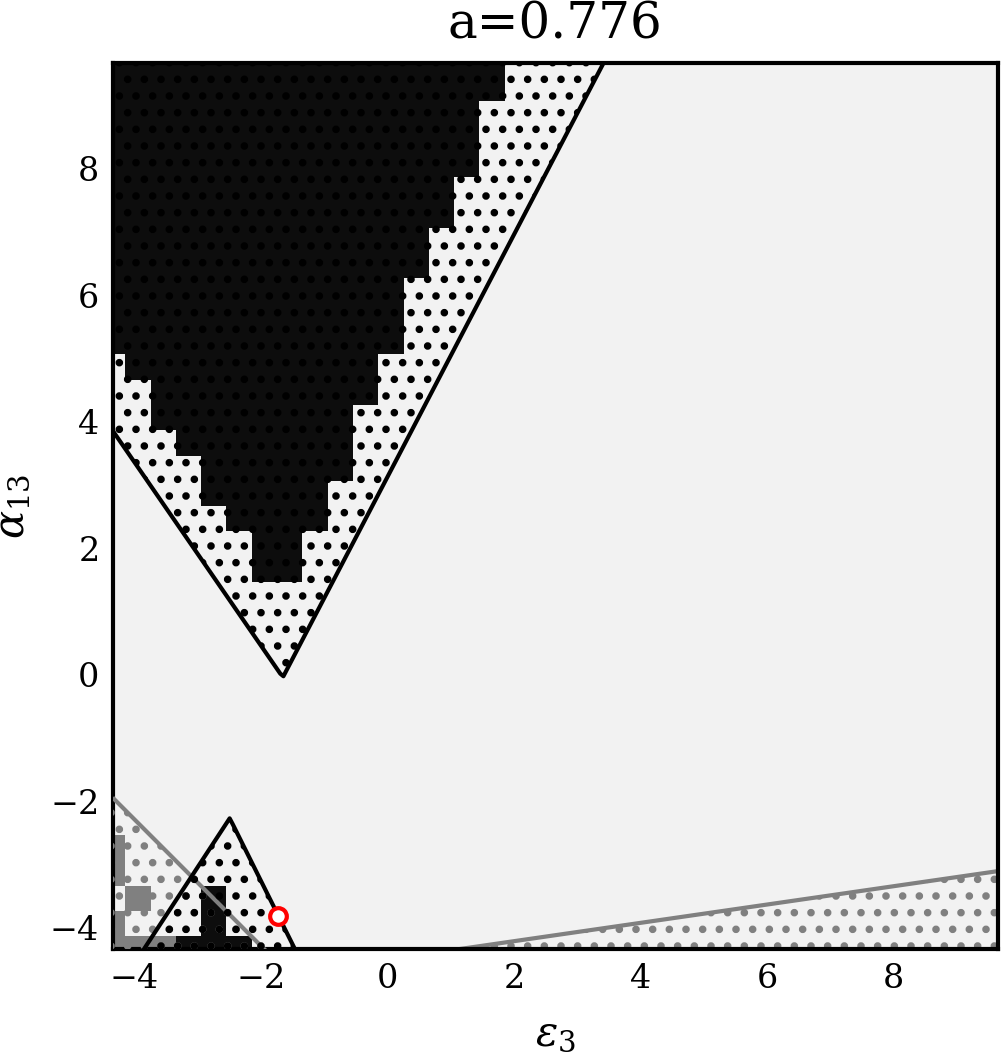
\includegraphics[keepaspectratio]{images/Fail12.png}}
\end{center}
\end{minipage}%
\newline
\begin{minipage}[t]{0.50\linewidth}
\begin{center}
\pandocbounded{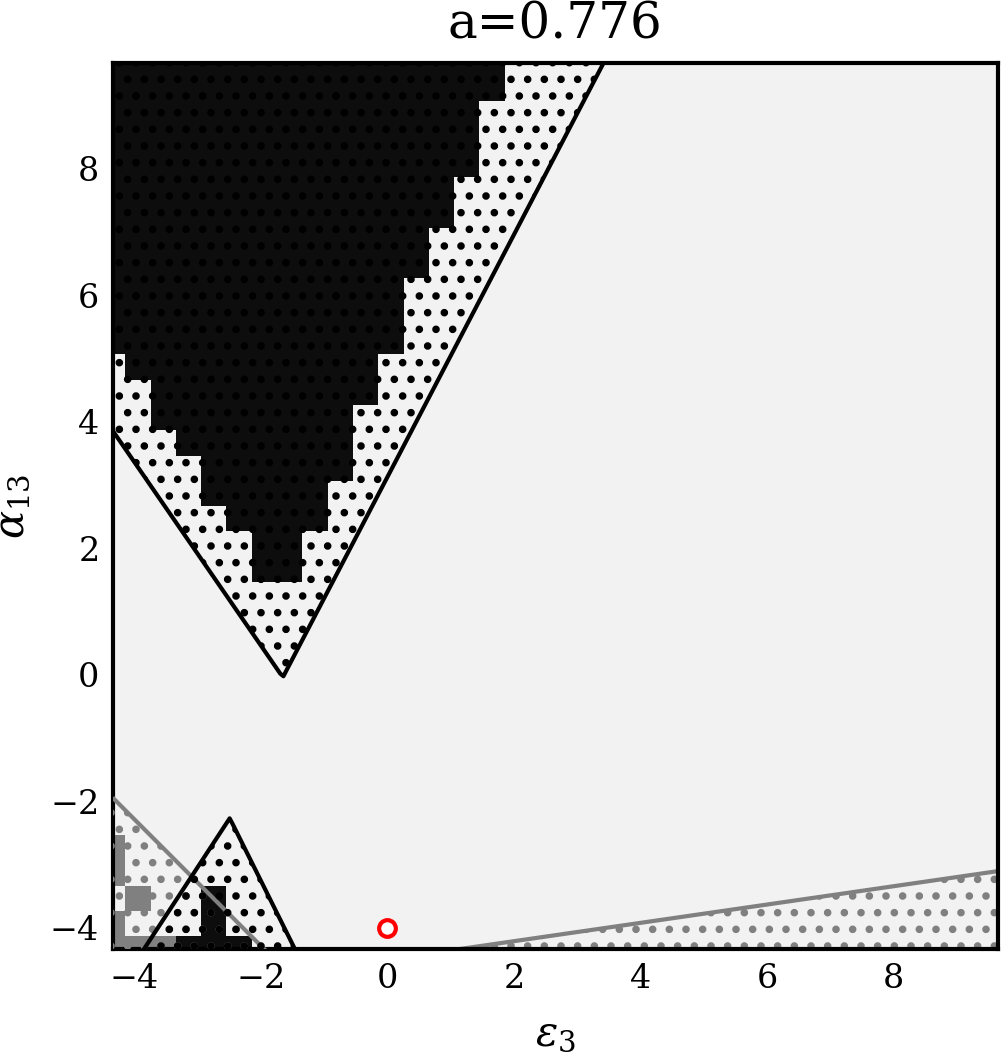
\includegraphics[keepaspectratio]{images/Fail13.png}}
\end{center}
\end{minipage}%
%
\begin{minipage}[t]{0.50\linewidth}
\begin{center}
\pandocbounded{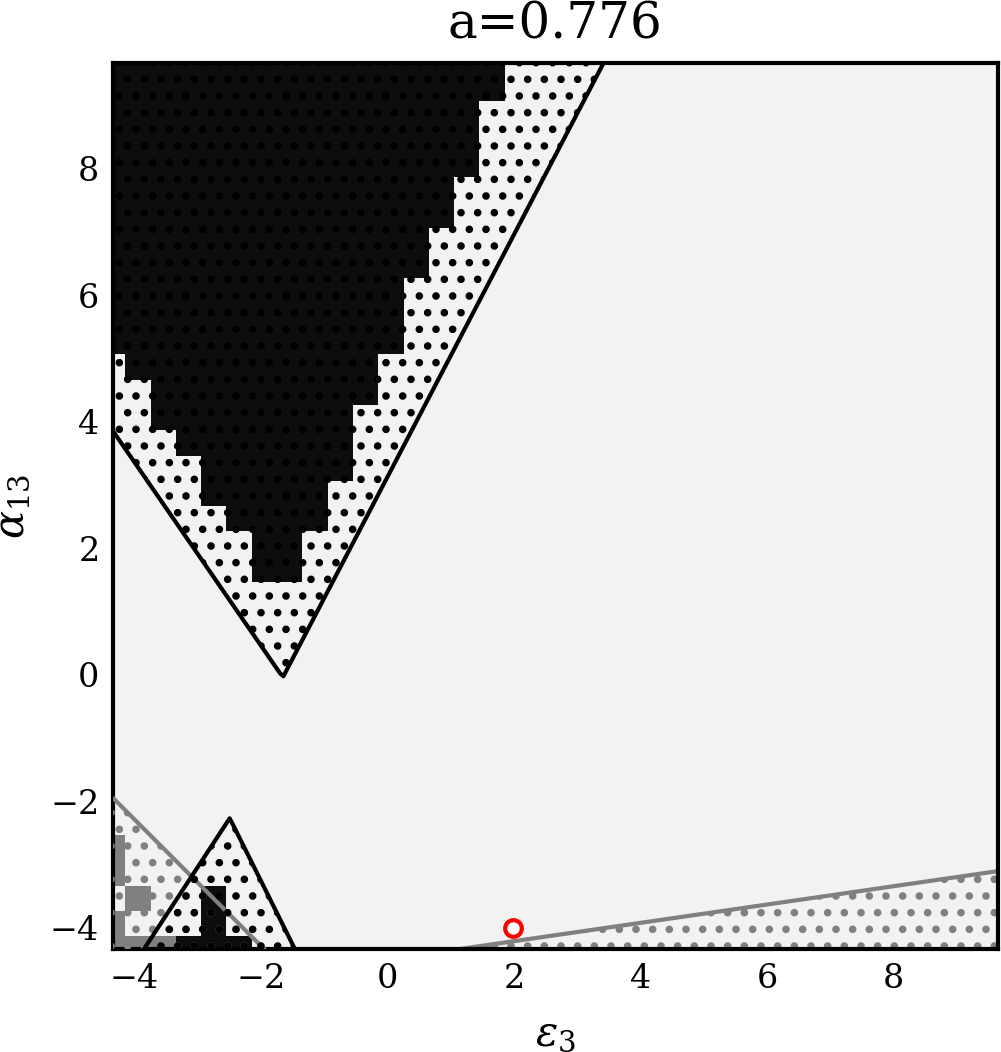
\includegraphics[keepaspectratio]{images/Fail14.png}}
\end{center}
\end{minipage}%
\newline
\begin{minipage}[t]{0.50\linewidth}
\begin{center}
\pandocbounded{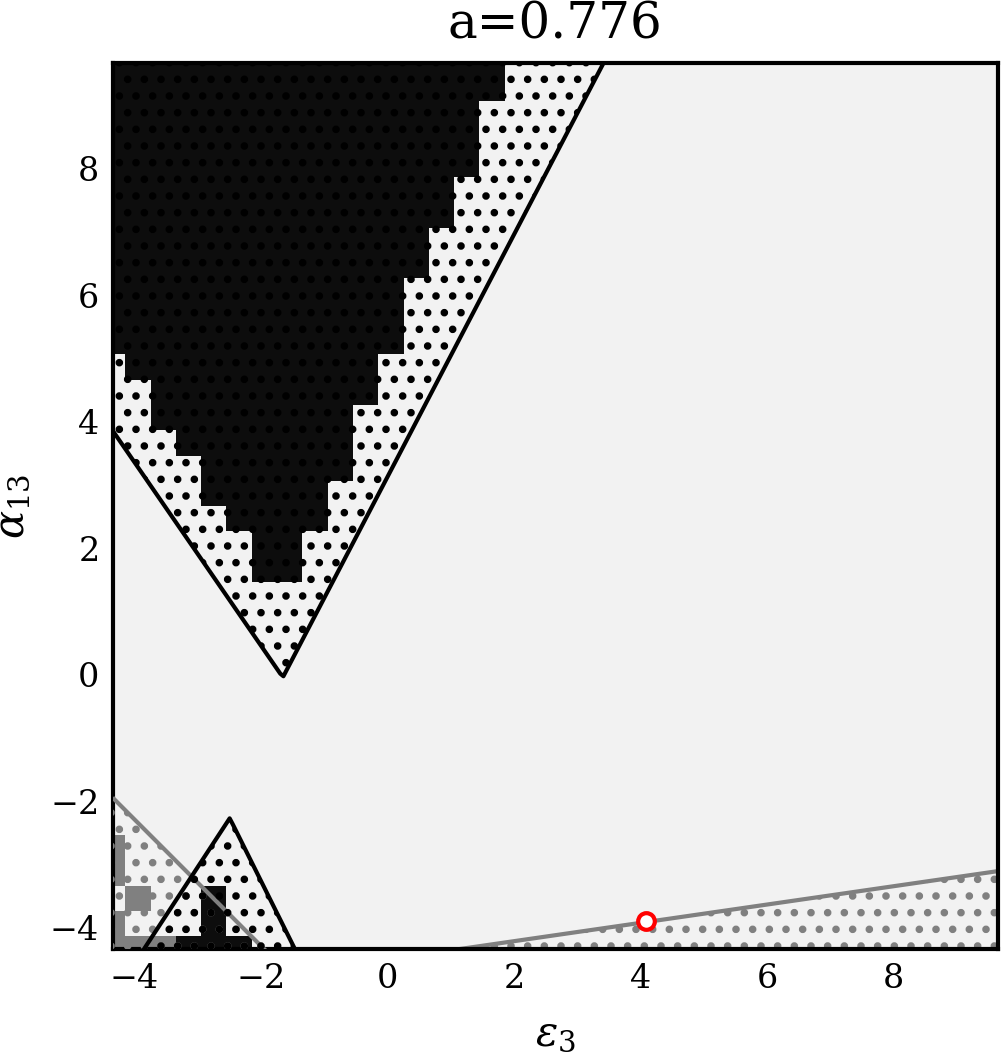
\includegraphics[keepaspectratio]{images/Fail15.png}}
\end{center}
\end{minipage}%

\end{figure}%

Given that the bad combinations consistently had low \(\alpha_{13}\), it
was possible to fix these errors by simply shifting the points upwards
slightly in parameter space. This of course increases the error in the
table model, however this can be quantified and was deemed necessary for
the purposes of this investigation. The table model was thus constructed
from a 5D grid with equally spaced points selected from the following
ranges

{\def\LTcaptype{none} % do not increment counter
\begin{longtable}[]{@{}llll@{}}
\toprule\noalign{}
Parameter & Lower Bound & Upper Bound & Number \\
\midrule\noalign{}
\endhead
\bottomrule\noalign{}
\endlastfoot
\(a\) & 0 & 0.998 & 10 \\
\(h\) & 1 & 15 & 10 \\
\(\theta\) & 5 & 85 & 9 \\
\(\alpha_{13}\) & -8 & 10 & 10 \\
\(\epsilon_{3}\) & -8 & 10 & 10 \\
\end{longtable}
}

\bookmarksetup{startatroot}

\chapter*{References}\label{references}
\addcontentsline{toc}{chapter}{References}

\markboth{References}{References}

\protect\phantomsection\label{refs}
\begin{CSLReferences}{0}{0}
\bibitem[\citeproctext]{ref-BroadIronLines}
\CSLLeftMargin{{[}1{]} }%
\CSLRightInline{\href{https://doi.org/10.1086/316610}{A. C. Fabian
\emph{et al.}, Publications of the Astronomical Society of the Pacific
\textbf{112}, 1145 (2000)}.}

\bibitem[\citeproctext]{ref-NuSTAR}
\CSLLeftMargin{{[}2{]} }%
\CSLRightInline{\href{https://doi.org/10.1088/0004-637X/770/2/103}{F. A.
Harrison \emph{et al.}, American Physical Journal \textbf{770}, 103
(2013)}.}

\bibitem[\citeproctext]{ref-JohannsenMetric}
\CSLLeftMargin{{[}3{]} }%
\CSLRightInline{\href{https://doi.org/10.1103/physrevd.88.044002}{T.
Johannsen, Physical Review D \textbf{88}, (2013)}.}

\bibitem[\citeproctext]{ref-XSPECModelSpecification}
\CSLLeftMargin{{[}4{]} }%
\CSLRightInline{K. A. Arnaud,
\emph{\href{https://heasarc.gsfc.nasa.gov/docs/heasarc/caldb/docs/memos/ogip_92_009/ogip_92_009.pdf}{The
File Format for XSPEC Table Models}} (NASA, 2021).}

\bibitem[\citeproctext]{ref-SpectralFitting}
\CSLLeftMargin{{[}5{]} }%
\CSLRightInline{\href{https://doi.org/10.5281/zenodo.17390971}{F. Baker
and A. Young, Zenodo (2025)}.}

\bibitem[\citeproctext]{ref-ConstrainingAlpha13}
\CSLLeftMargin{{[}6{]} }%
\CSLRightInline{\href{https://doi.org/10.1103/PhysRevD.99.083001}{A.
Tripathi \emph{et al.}, Phys. Rev. D \textbf{99}, 083001 (2019)}.}

\bibitem[\citeproctext]{ref-XRISMQSG}
\CSLLeftMargin{{[}7{]} }%
\CSLRightInline{XRISM Science Data Center,
\emph{\href{https://heasarc.gsfc.nasa.gov/docs/xrism/analysis/quickstart/xrism_quick_start_guide_v3p2_251204a.pdf}{XRISM
Quick-Start Guide}} (NASA, 2025).}

\bibitem[\citeproctext]{ref-xtdpixclip}
\CSLLeftMargin{{[}8{]} }%
\CSLRightInline{XRISM Science Data Center,
\emph{\href{https://heasarc.gsfc.nasa.gov/docs/xrism/analysis/quickstart/xtdpixclip_guide_v1p0_260106.pdf}{XRISM
Xtend Anomalous Pixels Clipper (Xtdpixclip) Special Topic Guide STG002}}
(NASA, 2026).}

\bibitem[\citeproctext]{ref-ISCOSpin}
\CSLLeftMargin{{[}9{]} }%
\CSLRightInline{\href{https://doi.org/10.1088/1742-6596/2012/1/012123}{S.
Liu, Journal of Physics: Conference Series \textbf{2012}, 012123
(2021)}.}

\end{CSLReferences}




\end{document}
